\documentclass[11pt]{article}
\usepackage[letterpaper,margin=1.05in]{geometry}
\usepackage[T1]{fontenc}
\usepackage[utf8]{inputenc}
\usepackage{lmodern}
\usepackage{microtype}
\usepackage{amsmath,amssymb,mathtools}
\usepackage{tikz}
\usepackage{enumitem}
\setlength{\parindent}{1.35em}
\setlength{\parskip}{0.15em}
\setlist[enumerate]{leftmargin=2.2em,itemsep=0.4em,topsep=0.4em}
\emergencystretch=2.5em
\allowdisplaybreaks
\newcommand{\dd}{\mathop{}\!d}
\newcommand{\eps}{\epsilon}
\newcommand{\D}{\Delta}
\newcommand{\unit}[1]{\mathfrak{S}_{#1}}
\newcommand{\ds}{\displaystyle}
\newcommand{\symfootnote}[2]{\begingroup\renewcommand{\thefootnote}{#1}\footnote{#2}\endgroup}
\begin{document}




\begin{center}
{\Large III.}\\[0.5em]
{\Large\scshape On the Equilibrium of Heterogeneous Substances}\\[0.5em]
{\small [\textit{Transactions of the Connecticut Academy}, III. pp. 108--248, Oct. 1875--May, 1876, and pp. 343--524, May, 1877--July, 1878.]}
\end{center}

\begin{quote}
``Die Energie der Welt ist constant.

Die Entropie der Welt strebt einem Maximum zu.''\par
\hfill Clausius.\footnote{\textit{Pogg. Ann.}, Bd. CXXV. (1865), S. 400; or \textit{Mechanische Wärmetheorie}, Abhand. ix. S. 44.}
\end{quote}

The comprehension of the laws which govern any material system is greatly facilitated by considering the energy and entropy of the system in the various states of which it is capable. As the difference of the values of the energy for any two states represents the combined amount of work and heat received or yielded by the system when it is brought from one state to the other, and the difference of entropy is the limit of all the possible values of the integral \(\int \frac{\dd Q}{t}\), \(\dd Q\) denoting the element of the heat received from external sources, and \(t\) the temperature of the part of the system receiving it, the varying values of the energy and entropy characterize in all that is essential the effects producible by the system in passing from one state to another. For by mechanical and thermodynamic contrivances, supposed theoretically perfect, any supply of work and heat may be transformed into any other which does not differ from it either in the amount of work and heat taken together or in the value of the integral \(\int\frac{\dd Q}{t}\). But it is not only in respect to the external relations of a system that its energy and entropy are of predominant importance. As in the case of simply mechanical systems, such as are discussed in theoretical mechanics, which are capable of only one kind of action upon external systems, viz., the performance of mechanical work, the function which expresses the capability of the system for this kind of action also plays the leading part in the theory of equilibrium, the condition of equilibrium being that the variation of this function shall vanish, so in a thermodynamic system, such as all material systems actually are, which is capable of two different kinds of action upon external systems, the two functions which express the twofold capabilities of the system afford an almost equally simple criterion of equilibrium.

\section*{Criteria of Equilibrium and Stability}

The criterion of equilibrium for a material system which is isolated from all external influences may be expressed in either of the following entirely equivalent forms:—

\begin{enumerate}[label=\Roman*.]
\item For the equilibrium of any isolated system it is necessary and sufficient that in all possible variations of the state of the system which do not alter its energy, the variation of its entropy shall either vanish or be negative. If \(\eps\) denote the energy, and \(\eta\) the entropy of the system, and we use a subscript letter after a variation to indicate a quantity of which the value is not to be varied, the condition of equilibrium may be written
\begin{equation}
(\delta\eta)_{\eps}\leq 0.
\end{equation}

\item For the equilibrium of any isolated system it is necessary and sufficient that in all possible variations in the state of the system which do not alter its entropy, the variation of its energy shall either vanish or be positive. This condition may be written
\begin{equation}
(\delta\eps)_{\eta}\geq 0.
\end{equation}
\end{enumerate}

That these two theorems are equivalent will appear from the consideration that it is always possible to increase both the energy and the entropy of the system, or to decrease both together, viz., by imparting heat to any part of the system or by taking it away. For, if condition (1) is not satisfied, there must be some variation in the state of the system for which
\[
\delta\eta>0 \quad\text{and}\quad \delta\eps=0;
\]
therefore, by diminishing both the energy and the entropy of the system in its varied state, we shall obtain a state for which, considered as a variation from the original state,
\[
\delta\eta=0 \quad\text{and}\quad \delta\eps<0;
\]
therefore condition (2) is not satisfied. Conversely, if condition (2) is not satisfied, there must be a variation in the state of the system for which
\[
\delta\eps<0 \quad\text{and}\quad \delta\eta=0;
\]
hence there must also be one for which
\[
\delta\eps=0 \quad\text{and}\quad \delta\eta>0;
\]
therefore condition (1) is not satisfied.

The equations which express the condition of equilibrium, as also its statement in words, are to be interpreted in accordance with the general usage in respect to differential equations, that is, infinitesimals of higher orders than the first relatively to those which express the amount of change of the system are to be neglected. But to distinguish the different kinds of equilibrium in respect to stability, we must have regard to the absolute values of the variations. We will use \(\D\) as the sign of variation in those equations which are to be construed strictly, i.e., in which infinitesimals of the higher orders are not to be neglected. With this understanding, we may express the necessary and sufficient conditions of the different kinds of equilibrium as follows;—for stable equilibrium
\begin{equation}
(\D\eta)_{\eps}<0,\quad \text{i.e.,}\quad (\D\eps)_{\eta}>0;
\end{equation}
for neutral equilibrium there must be some variations in the state of the system for which
\begin{equation}
(\D\eta)_{\eps}=0,\quad \text{i.e.,}\quad (\D\eps)_{\eta}=0;
\end{equation}
while in general
\begin{equation}
(\D\eta)_{\eps}\leq 0,\quad \text{i.e.,}\quad (\D\eps)_{\eta}\geq 0;
\end{equation}
and for unstable equilibrium there must be some variations for which
\begin{equation}
(\D\eta)_{\eps}>0,
\end{equation}
i.e., there must be some for which
\begin{equation}
(\D\eps)_{\eta}<0,
\end{equation}
while in general
\begin{equation}
(\delta\eta)_{\eps}\leq 0,\quad \text{i.e.,}\quad (\delta\eps)_{\eta}\geq 0.
\end{equation}

In these criteria of equilibrium and stability, account is taken only of possible variations. It is necessary to explain in what sense this is to be understood. In the first place, all variations in the state of the system which involve the transportation of any matter through any finite distance are of course to be excluded from consideration, although they may be capable of expression by infinitesimal variations of quantities which perfectly determine the state of the system. For example, if the system contains two masses of the same substance, not in contact, nor connected by other masses consisting of or containing the same substance or its components, an infinitesimal increase of the one mass with an equal decrease of the other is not to be considered as a possible variation in the state of the system. In addition to such cases of essential impossibility, if heat can pass by conduction or radiation from every part of the system to every other, only those variations are to be rejected as impossible, which involve changes which are prevented by passive forces or analogous resistances to change. But, if the system consist of parts between which there is supposed to be no thermal communication, it will be necessary to regard as impossible any diminution of the entropy of any of these parts, as such a change can not take place without the passage of heat. This limitation may most conveniently be applied to the second of the above forms of the condition of equilibrium, which will then become
\begin{equation}
(\delta\eps)_{\eta',\,\eta'',\,\mathrm{etc.}}\geq 0,
\end{equation}
\(\eta'\), \(\eta''\), etc., denoting the entropies of the various parts between which there is no communication of heat. When the condition of equilibrium is thus expressed, the limitation in respect to the conduction of heat will need no farther consideration.

In order to apply to any system the criteria of equilibrium which have been given, a knowledge is requisite of its passive forces or resistances to change, in so far, at least, as they are capable of preventing change. Those passive forces which only retard change, like viscosity, need not be considered. Such properties of a system are in general easily recognized upon the most superficial knowledge of its nature. As examples, we may instance the passive force of friction which prevents sliding when two surfaces of solids are pressed together,—that which prevents the different components of a solid, and sometimes of a fluid, from having different motions one from another,—that resistance to change which sometimes prevents either of two forms of the same substance, simple or compound, which are capable of existing, from passing into the other,—that which prevents the changes in solids which imply plasticity, in other words, changes of the form to which the solid tends to return, when the deformation does not exceed certain limits.

It is a characteristic of all these passive resistances that they prevent a certain kind of motion or change, however the initial state of the system may be modified, and to whatever external agencies of force and heat it may be subjected, within limits, it may be, but yet within limits which allow finite variations in the values of all the quantities which express the initial state of the system or the mechanical or thermal influences acting on it, without producing the change in question. The equilibrium which is due to such passive properties is thus widely distinguished from that caused by the balance of the active tendencies of the system, where an external influence, or a change in the initial state, infinitesimal in amount, is sufficient to produce change either in the positive or negative direction. Hence the ease with which these passive resistances are recognized. Only in the case that the state of the system lies so near the limit at which the resistances cease to be operative to prevent change, as to create a doubt whether the case falls within or without the limit, will a more accurate knowledge of these resistances be necessary.

To establish the validity of the criterion of equilibrium, we will consider first the sufficiency, and afterwards the necessity, of the condition as expressed in either of the two equivalent forms.

In the first place, if the system is in a state in which its entropy is greater than in any other state of the same energy, it is evidently in equilibrium, as any change of state must involve either a decrease of entropy or an increase of energy, which are alike impossible for an isolated system. We may add that this is a case of stable equilibrium, as no infinitely small cause, whether relating to a variation of the initial state or to the action of any external bodies, can produce a finite change of state, as this would involve a finite decrease of entropy or increase of energy.

We will next suppose that the system has the greatest entropy consistent with its energy, and therefore the least energy consistent with its entropy, but that there are other states of the same energy and entropy as its actual state. In this case, it is impossible that any motion of masses should take place; for if any of the energy of the system should come to consist of vis viva, of sensible motions, a state of the system identical in other respects but without the motion would have less energy and not less entropy, which would be contrary to the supposition. But we cannot apply this reasoning to the motion within any mass of its different components in different directions, as in diffusion, when the momenta of the components balance one another. Nor, in the case supposed, can any conduction of heat take place, for this involves an increase of entropy, as heat is only conducted from bodies of higher to those of lower temperature. It is equally impossible that any changes should be produced by the transfer of heat by radiation. The condition which we have supposed is therefore sufficient for equilibrium, so far as the motion of masses and the transfer of heat are concerned, but to show that the same is true in regard to the motions of diffusion and chemical or molecular changes, when these can occur without being accompanied or followed by the motions of masses or the transfer of heat, we must have recourse to considerations of a more general nature. The following considerations seem to justify the belief that the condition is sufficient for equilibrium in every respect.

Let us suppose, in order to test the stability of such a hypothesis, that a system may have the greatest entropy consistent with its energy without being in equilibrium. In such a case, changes in the state of the system must take place, but these will necessarily be such that the energy and the entropy will each remain constant, and the system will continue to satisfy the same condition, as initially, of having the greatest entropy consistent with its energy. Let us consider the change which takes place in any time so short that the state of the system may be regarded as uniform in nature throughout that time. This time must be so chosen that the change does not take place infinitely slowly, which is always easy, as the change which we suppose to take place cannot be infinitely slow except at particular moments. Now no change whatever in the state of the system, which does not alter the value of the energy, and which commences with the same state in which the system was supposed at the commencement of the short time considered, will cause an increase of entropy. Hence, it will generally be possible by some slight variation in the circumstances of the case to make all changes in the state of the system like or nearly like that which is supposed actually to occur, and not involving a change of energy, to involve a necessary decrease of entropy, which would render any such change impossible. This variation may be in the values of the variables which determine the state of the system, or in the values of the constants which determine the nature of the system, or in the form of the functions which express its laws,—only there must be nothing in the system as modified which is thermodynamically impossible. For example, we might suppose temperature or pressure to be varied, or the composition of the different bodies in the system, or, if no small variations which could be actually realized would produce the required result, we might suppose the properties themselves of the substances to undergo variation, subject to the general laws of matter. If, then, there is any tendency toward change in the system as first supposed, it is a tendency which can be entirely checked by an infinitesimal variation in the circumstances of the case. As this supposition cannot be allowed, we must believe that a system is always in equilibrium when it has the greatest entropy consistent with its energy, or, in other words, when it has the least energy consistent with its entropy.

The same considerations will evidently apply to any case in which a system is in such a state that \(\D\eta=0\) for any possible infinitesimal variation of the state for which \(\D\eps=0\), even if the entropy is not the greatest of which the system is capable with the same energy. The term possible has here the meaning previously defined, and the character \(\D\) is used, as before, to denote that the equation is to be construed strictly, i.e., without neglect of the infinitesimals of the higher orders.

The only case in which the sufficiency of the condition of equilibrium which has been given remains to be proved is that in which in our notation \((\delta\eta)_{\eps}\leq 0\) for all possible variations not affecting the energy, but for some of these variations \(\D\eta>0\), that is, when the entropy has in some respects the characteristics of a minimum. In this case the considerations adduced in the last paragraph will not apply without modification, as the change of state may be infinitely slow at first, and it is only in the initial state that the condition \((\delta\eta)_{\eps}\leq 0\) holds true. But the differential coefficients of all orders of the quantities which determine the state of the system, taken with respect of the time, must be functions of these same quantities. None of these differential coefficients can have any value other than 0, for the state of the system for which \((\delta\eta)_{\eps}\leq 0\). For otherwise, as it would generally be possible, as before, by some infinitely small modification of the case, to render impossible any change like or nearly like that which might be supposed to occur, this infinitely small modification of the case would make a finite difference in the value of the differential coefficients which had before the finite values, or in some of lower orders, which is contrary to that continuity which we have reason to expect. Such considerations seem to justify us in regarding such a state as we are discussing as one of theoretical equilibrium; although as the equilibrium is evidently unstable, it cannot be realized.

We have still to prove that the condition enunciated is in every case necessary for equilibrium. It is evidently so in all cases in which the active tendencies of the system are so balanced that changes of every kind, except those excluded in the statement of the condition of equilibrium, can take place reversibly, i.e., both in the positive and the negative direction, in states of the system differing infinitely little from the state in question. In this case, we may omit the sign of inequality and write as the condition of such a state of equilibrium
\begin{equation}
(\delta\eta)_{\eps}=0,\quad \text{i.e.,}\quad (\delta\eps)_{\eta}=0.
\end{equation}
But to prove that the condition previously enunciated is in every case necessary, it must be shown that whenever an isolated system remains without change, if there is any infinitesimal variation in its state, not involving a finite change of position of any, even an infinitesimal part, of its matter, which would diminish its energy by a quantity which is not infinitely small relatively to the variations of the quantities which determine the state of the system, without altering its entropy,—or, if the system has thermally isolated parts, without altering the entropy of any such part,—this variation involves changes in the system which are prevented by its passive forces or analogous resistances to change. Now, as the described variation in the state of the system diminishes its energy without altering its entropy, it must be regarded as theoretically possible to produce that variation by some process, perhaps a very indirect one, so as to gain a certain amount of work above all expended on the system. Hence we may conclude that the active forces or tendencies of the system favor the variation in question, and that equilibrium cannot subsist unless the variation is prevented by passive forces.

The preceding considerations will suffice, it is believed, to establish the validity of the criterion of equilibrium which has been given. The criteria of stability may readily be deduced from that of equilibrium. We will now proceed to apply these principles to systems consisting of heterogeneous substances and deduce the special laws which apply to different classes of phenomena. For this purpose we shall use the second form of the criterion of equilibrium, both because it admits more readily the introduction of the condition that there shall be no thermal communication between the different parts of the system, and because it is more convenient, as respects the form of the general equations relating to equilibrium, to make the entropy one of the independent variables which determine the state of the system, than to make the energy one of these variables.

\section*{The Conditions of Equilibrium for Heterogeneous Masses in Contact when Uninfluenced by Gravity, Electricity, Distortion of the Solid Masses, or Capillary Tensions}

In order to arrive as directly as possible at the most characteristic and essential laws of chemical equilibrium, we will first give our attention to a case of the simplest kind. We will examine the conditions of equilibrium of a mass of matter of various kinds enclosed in a rigid and fixed envelop, which is impermeable to and unalterable by any of the substances enclosed, and perfectly non-conducting to heat. We will suppose that the case is not complicated by the action of gravity, or by any electrical influences, and that in the solid portions of the mass the pressure is the same in every direction. We will farther simplify the problem by supposing that the variations of the parts of the energy and entropy which depend upon the surfaces separating heterogeneous masses are so small in comparison with the variations of the parts of the energy and entropy which depend upon the quantities of these masses, that the former may be neglected by the side of the latter; in other words, we will exclude the considerations which belong to the theory of capillarity.

It will be observed that the supposition of a rigid and non-conducting envelop enclosing the mass under discussion involves no real loss of generality, for if any mass of matter is in equilibrium, it would also be so, if the whole or any part of it were enclosed in an envelop as supposed; therefore the conditions of equilibrium for a mass thus enclosed are the general conditions which must always be satisfied in case of equilibrium. As for the other suppositions which have been made, all the circumstances and considerations which are here excluded will afterward be made the subject of special discussion.

\subsection*{Conditions relating to the Equilibrium between the initially existing Homogeneous Parts of the given Mass}

Let us first consider the energy of any homogeneous part of the given mass, and its variation for any possible variation in the composition and state of this part. By homogeneous is meant that the part in question is uniform throughout, not only in chemical composition, but also in physical state. If we consider the amount and kind of matter in this homogeneous mass as fixed, its energy \(\eps\) is a function of its entropy \(\eta\), and its volume \(v\), and the differentials of these quantities are subject to the relation
\begin{equation}
\dd\eps = t\,\dd\eta - p\,\dd v,
\end{equation}
\(t\) denoting the absolute temperature of the mass, and \(p\) its pressure. For \(t\,\dd\eta\) is the heat received, and \(p\,\dd v\) the work done, by the mass during its change of state. But if we consider the matter in the mass as variable, and write \(m_1,m_2,\ldots,m_n\) for the quantities of the various substances \(S_1,S_2,\ldots,S_n\) of which the mass is composed, \(\eps\) will evidently be a function of \(\eta,v,m_1,m_2,\ldots,m_n\), and we shall have for the complete value of the differential of \(\eps\)
\begin{equation}
\dd\eps
= t\,\dd\eta - p\,\dd v
  + \mu_1\,\dd m_1 + \mu_2\,\dd m_2 + \cdots + \mu_n\,\dd m_n,
\end{equation}
\(\mu_1,\mu_2,\ldots,\mu_n\) denoting the differential coefficients of \(\eps\) taken with respect to \(m_1,m_2,\ldots,m_n\).

The substances \(S_1,S_2,\ldots,S_n\), of which we consider the mass composed, must of course be such that the values of the differentials \(\dd m_1,\dd m_2,\ldots,\dd m_n\) shall be independent, and shall express every possible variation in the composition of the homogeneous mass considered, including those produced by the absorption of substances different from any initially present. It may therefore be necessary to have terms in the equation relating to component substances which do not initially occur in the homogeneous mass considered, provided, of course, that these substances, or their components, are to be found in some part of the whole given mass.

If the conditions mentioned are satisfied, the choice of the substances which we are to regard as the components of the mass considered may be determined entirely by convenience, and independently of any theory in regard to the internal constitution of the mass. The number of components will sometimes be greater, and sometimes less, than the number of chemical elements present. For example, in considering the equilibrium in a vessel containing water and free hydrogen and oxygen, we should be obliged to recognize three components in the gaseous part. But in considering the equilibrium of dilute sulphuric acid with the vapor which it yields, we should have only two components to consider in the liquid mass, sulphuric acid, anhydrous, or of any particular degree of concentration, and additional water. If, however, we are considering sulphuric acid in a state of maximum concentration in connection with substances which might possibly afford water to the acid, it must be noticed that the condition of the independence of the differentials will require that we consider the acid in the state of maximum concentration as one of the components. The quantity of this component will then be capable of variation both in the positive and in the negative sense, while the quantity of the other component can increase but cannot decrease below the value 0.

For brevity's sake, we may call a substance \(S_a\) an actual component of any homogeneous mass, to denote that the quantity \(m_a\) of that substance in the given mass may be either increased or diminished, although we may have so chosen the other component substances that \(m_a=0\); and we may call a substance \(S_b\) a possible component to denote that it may be combined with, but cannot be subtracted from the homogeneous mass in question. In this case, as we have seen in the above example, we must so choose the component substances that \(m_b=0\).

The units by which we measure the substances of which we regard the given mass as composed may each be chosen independently. To fix our ideas for the purpose of a general discussion, we may suppose all substances measured by weight or mass. Yet in special cases, it may be more convenient to adopt chemical equivalents as the units of the component substances.

It may be observed that it is not necessary for the validity of equation (12) that the variations of nature and state of the mass to which the equation refers should be such as do not disturb its homogeneity, provided that in all parts of the mass the variations of nature and state are infinitely small. For, if this last condition be not violated, an equation like (12) is certainly valid for all the infinitesimal parts of the initially homogeneous mass; i.e., if we write \(D\eps,D\eta\), etc., for the energy, entropy, etc., of any infinitesimal part,
\begin{equation}
\dd D\eps
= t\,\dd D\eta - p\,\dd Dv
  + \mu_1\,\dd Dm_1 + \mu_2\,\dd Dm_2 + \cdots + \mu_n\,\dd Dm_n,
\end{equation}
whence we may derive equation (12) by integrating for the whole initially homogeneous mass.

We will now suppose that the whole mass is divided into parts so that each part is homogeneous, and consider such variations in the energy of the system as are due to variations in the composition and state of the several parts remaining, at least approximately, homogeneous, and together occupying the whole space within the envelop. We will at first suppose the case to be such that the component substances are the same for each of the parts, each of the substances \(S_1,S_2,\ldots,S_n\) being an actual component of each part. If we distinguish the letters referring to the different parts by accents, the variation in the energy of the system may be expressed by \(\delta\eps' + \delta\eps'' + \cdots\), and the general condition of equilibrium requires that
\begin{equation}
\delta\eps' + \delta\eps'' + \cdots \geq 0.
\end{equation}



for all variations which do not conflict with the equations of condition. These equations must express that the entropy of the whole given mass does not vary, nor its volume, nor the total quantities of any of the substances \(S_1,S_2,\ldots,S_n\). We will suppose that there are no other equations of condition. It will then be necessary for equilibrium that
\begin{equation}
\begin{aligned}
&t'\delta\eta' - p'\delta v'
  + \mu_1'\delta m_1' + \mu_2'\delta m_2' + \cdots
  + \mu_n'\delta m_n' \\
&\quad
 + t''\delta\eta'' - p''\delta v''
  + \mu_1''\delta m_1'' + \mu_2''\delta m_2'' + \cdots
  + \mu_n''\delta m_n''
 + \cdots \geq 0
\end{aligned}
\end{equation}
for any values of the variations for which
\begin{equation}
\delta\eta' + \delta\eta'' + \delta\eta''' + \cdots =0,
\end{equation}
\begin{equation}
\delta v' + \delta v'' + \delta v''' + \cdots =0,
\end{equation}
\begin{equation}
\left.
\begin{aligned}
\delta m_1' + \delta m_1'' + \delta m_1''' + \cdots &=0,\\
\delta m_2' + \delta m_2'' + \delta m_2''' + \cdots &=0,\\
&\vdots\\
\delta m_n' + \delta m_n'' + \delta m_n''' + \cdots &=0.
\end{aligned}
\right\}
\end{equation}
For this it is evidently necessary and sufficient that
\begin{equation}
t'=t''=t'''=\cdots
\end{equation}
\begin{equation}
p'=p''=p'''=\cdots
\end{equation}
\begin{equation}
\left.
\begin{aligned}
\mu_1'&=\mu_1''=\mu_1'''=\cdots,\\
\mu_2'&=\mu_2''=\mu_2'''=\cdots,\\
&\vdots\\
\mu_n'&=\mu_n''=\mu_n'''=\cdots.
\end{aligned}
\right\}
\end{equation}

Equations (19) and (20) express the conditions of thermal and mechanical equilibrium, viz., that the temperature and the pressure must be constant throughout the whole mass. In equations (21) we have the conditions characteristic of chemical equilibrium. If we call a quantity \(\mu_x\), as defined by such an equation as (12), the potential for the substance \(S_x\) in the homogeneous mass considered, these conditions may be expressed as follows:—

The potential for each component substance must be constant throughout the whole mass.

It will be remembered that we have supposed that there is no restriction upon the freedom of motion or combination of the component substances, and that each is an actual component of all parts of the given mass.

The state of the whole mass will be completely determined, if we regard as immaterial the position and form of the various homogeneous parts of which it is composed, when the values are determined of the quantities of which the variations occur in (15). The number of these quantities, which we may call the independent variables, is evidently \((n+2)\nu\), \(\nu\) denoting the number of homogeneous parts into which the whole mass is divided. All the quantities which occur in (19), (20), (21), are functions of these variables, and may be regarded as known functions, if the energy of each part is known as a function of its entropy, volume, and the quantities of its components. See equation (12). Therefore, equations (19), (20), (21), may be regarded as \((\nu-1)(n+2)\) independent equations between the independent variables. The volume of the whole mass and the total quantities of the various substances being known afford \(n+1\) additional equations. If we also know the total energy of the given mass, or its total entropy, we will have as many equations as there are independent variables.

But if any of the substances \(S_1,S_2,\ldots,S_n\) are only possible components of some parts of the given mass, the variation \(\delta m\) of the quantity of such a substance in such a part cannot have a negative value, so that the general condition of equilibrium (15) does not require that the potential for that substance in that part should be equal to the potential for the same substance in the parts of which it is an actual component, but only that it shall not be less. In this case instead of (21) we may write
\begin{equation}
\left.
\begin{aligned}
\mu_1&=M_1 &&\text{for all parts of which \(S_1\) is an actual component, and}\\
\mu_1&\geq M_1 &&\text{for all parts of which \(S_1\) is a possible (but not actual) component,}\\[0.25em]
\mu_2&=M_2 &&\text{for all parts of which \(S_2\) is an actual component, and}\\
\mu_2&\geq M_2 &&\text{for all parts of which \(S_2\) is a possible (but not actual) component,}\\
&\vdots
\end{aligned}
\right\}
\end{equation}
\(M_1,M_2,\ldots\), denoting constants of which the value is only determined by these equations.

If we now suppose that the components, actual or possible, of the various homogeneous parts of the given mass are not the same, the result will be of the same character as before, provided that all the different components are independent, i.e., that no one can be made out of the others, so that the total quantity of each component is fixed. The general condition of equilibrium (15) and the equations of condition (16), (17), (18) will require no change, except that, if any of the substances \(S_1,S_2,\ldots,S_n\) is not a component, actual or possible, of any part, the term \(\mu\,\delta m\) for that substance and part will be wanting in the former, and the \(\delta m\) in the latter. This will require no change in the form of the particular conditions of equilibrium as expressed by (19), (20), (22); but the number of single conditions contained in (22) is of course less than if all the component substances were components of all the parts. Whenever, therefore, each of the different homogeneous parts of the given mass may be regarded as composed of some or of all of the same set of substances, no one of which can be formed out of the others, the condition which, with equality of temperature and pressure, is necessary and sufficient for equilibrium between the different parts of the given mass may be expressed as follows:—

The potential for each of the component substances must have a constant value in all parts of the given mass of which that substance is an actual component, and have a value not less than this in all parts of which it is a possible component.

The number of equations afforded by these conditions, after elimination of \(M_1,M_2,\ldots,M_n\), will be less than \((n+2)(\nu-1)\) by the number of terms in (15) in which the variation of the form \(\delta m\) is either necessarily nothing or incapable of a negative value. The number of variables to be determined is diminished by the same number, or, if we choose, we may write an equation of the form \(m=0\) for each of these terms. But when the substance is a possible component of the part concerned, there will also be a condition, expressed by \(\geq\), to show whether the supposition that the substance is not an actual component is consistent with equilibrium.

We will now suppose that the substances \(S_1,S_2,\ldots,S_n\) are not all independent of each other, i.e., that some of them can be formed out of others. We will first consider a very simple case. Let \(S_3\) be composed of \(S_1\) and \(S_2\) combined in the ratio of \(a\) to \(b\), \(S_1\) and \(S_2\) occurring as actual components in some parts of the given mass, and \(S_3\) in other parts, which do not contain \(S_1\) and \(S_2\) as separately variable components. The general condition of equilibrium will still have the form of (15) with certain of the terms of the form \(\mu\,\delta m\) omitted. It may be written more briefly
\begin{equation}
\sum(t\,\delta\eta)-\sum(p\,\delta v)
+\sum(\mu_1\delta m_1)+\sum(\mu_2\delta m_2)+\cdots
+\sum(\mu_n\delta m_n)\geq 0,
\end{equation}
the sign \(\sum\) denoting summation in regard to the different parts of the given mass. But instead of the three equations of condition,
\begin{equation}
\sum\delta m_1=0,\quad
\sum\delta m_2=0,\quad
\sum\delta m_3=0,
\end{equation}
we shall have the two,
\begin{equation}
\left.
\begin{aligned}
\sum\delta m_1 + {a\over a+b}\sum\delta m_3&=0,\\
\sum\delta m_2 + {b\over a+b}\sum\delta m_3&=0.
\end{aligned}
\right\}
\end{equation}
The other equations of condition,
\begin{equation}
\sum\delta\eta=0,\quad \sum\delta v=0,\quad \sum\delta m_4=0,\quad \text{etc.},
\end{equation}
will remain unchanged. Now as all values of the variations which satisfy equations (24) will also satisfy equations (25), it is evident that all the particular conditions of equilibrium which we have already deduced, (19), (20), (22), are necessary in this case also. When these are satisfied, the general condition (23) reduces to
\begin{equation}
M_1\sum\delta m_1+M_2\sum\delta m_2+M_3\sum\delta m_3\geq 0.
\end{equation}
For, although it may be that \(\mu_1'\), for example, is greater than \(M_1\), yet it can only be so when the following \(\delta m_1'\) is incapable of a negative value. Hence, if (27) is satisfied, (23) must also be. Again, if (23) is satisfied, (27) must also be satisfied, so long as the variation of the quantity of every substance has the value 0 in all the parts of which it is not an actual component. But as this limitation does not affect the range of the possible values of \(\sum\delta m_1\), \(\sum\delta m_2\), and \(\sum\delta m_3\), it may be disregarded. Therefore the conditions (23) and (27) are entirely equivalent, when (19), (20), (22) are satisfied. Now, by means of the equations of condition (25), we may eliminate \(\sum\delta m_1\) and \(\sum\delta m_2\) from (27), which becomes
\begin{equation}
-aM_1\sum\delta m_3-bM_2\sum\delta m_3
+(a+b)M_3\sum\delta m_3\geq 0,
\end{equation}
i.e., as the value of \(\sum\delta m_3\) may be either positive or negative,
\begin{equation}
aM_1+bM_2=(a+b)M_3,
\end{equation}
which is the additional condition of equilibrium which is necessary in this case.

The relations between the component substances may be less simple than in this case, but in any case they will only affect the equations of condition, and these may always be found without difficulty, and will enable us to eliminate from the general condition of equilibrium as many variations as there are equations of condition, after which the coefficients of the remaining variations may be set equal to zero, except the coefficients of variations which are incapable of negative values, which coefficients must be equal to or greater than zero. It will be easy to perform these operations in each particular case, but it may be interesting to see the form of the resultant equations in general.

We will suppose that the various homogeneous parts are considered as having in all \(n\) components, \(S_1,S_2,\ldots,S_n\), and that there is no restriction upon their freedom of motion and combination. But we will so far limit the generality of the problem as to suppose that each of these components is an actual component of some part of the given mass.\footnote{When we come to seek the conditions of equilibrium relating to the formation of masses unlike any previously existing, we shall take up \textit{de novo} the whole problem of the equilibrium of heterogeneous masses enclosed in a non-conducting envelop, and give it a more general treatment, which will be free from this limitation.} If some of these components can be formed out of others, all such relations can be expressed by equations such as
\begin{equation}
\alpha\unit{a}+\beta\unit{b}+\text{etc.}
=\kappa\unit{k}+\lambda\unit{l}+\text{etc.}
\end{equation}
where \(\unit{a},\unit{b},\unit{k}\), etc. denote the units of the substances \(S_a,S_b,S_k\), etc., that is, of certain of the substances \(S_1,S_2,\ldots,S_n\), and \(\alpha,\beta,\kappa,\lambda\), etc. denote numbers. These are not, it will be observed, equations between abstract quantities, but the sign \(=\) denotes qualitative as well as quantitative equivalence. We will suppose that there are \(r\) independent equations of this character. The equations of condition relating to the component substances may easily be derived from these equations, but it will not be necessary to consider them particularly. It is evident that they will be satisfied by any values of the variations which satisfy equations (18); hence, the particular conditions of equilibrium (19), (20), (22) must be necessary in this case, and, if these are satisfied, the general equation of equilibrium (15) or (23) will reduce to
\begin{equation}
M_1\sum\delta m_1+M_2\sum\delta m_2+\cdots+M_n\sum\delta m_n\geq 0.
\end{equation}
This will appear from the same considerations which were used in regard to equations (23) and (27). Now it is evidently possible to give to \(\sum\delta m_a,\sum\delta m_b,\sum\delta m_k\), etc. values proportional to \(\alpha,\beta,-\kappa\), etc. in equation (30), and also the same values taken negatively, making \(\sum\delta m=0\) in each of the other terms; therefore
\begin{equation}
\alpha M_a+\beta M_b+\text{etc.}-\kappa M_k-\lambda M_l-\text{etc.}=0,
\end{equation}
or,
\begin{equation}
\alpha M_a+\beta M_b+\text{etc.}=\kappa M_k+\lambda M_l+\text{etc.}
\end{equation}
It will be observed that this equation has the same form and coefficients as equation (30), \(M\) taking the place of \(\mathfrak S\). It is evident that there must be a similar condition of equilibrium for every one of the \(r\) equations of which (30) is an example, which may be obtained simply by changing \(\mathfrak S\) in these equations into \(M\). When these conditions are satisfied, (31) will be satisfied with any possible values of \(\sum\delta m_1,\sum\delta m_2,\ldots,\sum\delta m_n\). For no values of these quantities are possible, except such that the equation
\begin{equation}
(\sum\delta m_1)\unit{1}+(\sum\delta m_2)\unit{2}+\cdots+(\sum\delta m_n)\unit{n}=0,
\end{equation}
after the substitution of these values, can be derived from the \(r\) equations like (30), by the ordinary processes of the reduction of linear equations. Therefore, on account of the correspondence between (31) and (34), and between the \(r\) equations like (33) and the \(r\) equations like (30), the conditions obtained by giving any possible values to the variations in (31) may also be derived from the \(r\) equations like (33); that is, the condition (31) is satisfied if the \(r\) equations like (33) are satisfied. Therefore the \(r\) equations like (33) are with (19), (20), and (22) the equivalent of the general condition (15) or (23).

For determining the state of a given mass when in equilibrium and having a given volume and given energy or entropy, the condition of equilibrium affords an additional equation corresponding to each of the \(r\) independent relations between the \(n\) component substances. But the equations which express our knowledge of the matter in the given mass will be correspondingly diminished, being \(n-r\) in number, like the equations of condition relating to the quantities of the component substances, which may be derived from the former by differentiation.

\section*{Conditions relating to the possible Formation of Masses Unlike any Previously Existing}

The variations which we have hitherto considered do not embrace every possible infinitesimal variation in the state of the given mass, so that the particular conditions already formed, although always necessary for equilibrium, when there are no other equations of condition than such as we have supposed, are not always sufficient. For, besides the infinitesimal variations in the state and composition of different parts of the given mass, infinitesimal masses may be formed entirely different in state and composition from any initially existing. Such parts of the whole mass in its varied state as cannot be regarded as parts of the initially existing mass which have been infinitesimally varied in state and composition, we will call new parts. These will necessarily be infinitely small. As it is more convenient to regard a vacuum as a limiting case of extreme rarefaction than to give a special consideration to the possible formation of empty spaces within the given mass, the term new parts will be used to include any empty spaces which may be formed, when such have not existed initially. We will use \(D\epsilon,D\eta,Dv,Dm_1,Dm_2,\ldots,Dm_n\) to denote the infinitesimal energy, entropy, and volume of any one of these new parts, and the infinitesimal quantities of its components. The component substances \(S_1,S_2,\ldots,S_n\) must now be taken to include not only the independently variable components, actual or possible, of all parts of the given mass as initially existing, but also the components of all the new parts, the possible formation of which we have to consider. The character \(\delta\) will be used as before to express the infinitesimal variations of the quantities relating to those parts which are only infinitesimally varied in state and composition, and which for distinction we will call original parts, including under this term the empty spaces, if such exist initially, within the envelop bounding the system. As we may divide the given mass into as many parts as we choose, and as not only the initial boundaries, but also the movements of these boundaries during any variation in the state of the system are arbitrary, we may so define the parts which we have called original, that we may consider them as initially homogeneous and remaining so, and as initially constituting the whole system.

The most general value of the variation of the energy of the whole system is evidently
\begin{equation}
\sum\delta\epsilon+\sum D\epsilon,
\end{equation}
the first summation relating to all the original parts, and the second to all the new parts. Throughout the discussion of this problem, the letter \(\delta\) or \(D\) following \(\sum\) will sufficiently indicate whether the summation relates to the original or to the new parts. Therefore the general condition of equilibrium is
\begin{equation}
\sum\delta\epsilon+\sum D\epsilon\geq 0,
\end{equation}
or, if we substitute the value of \(\delta\epsilon\) taken from equation (12),
\begin{equation}
\sum D\epsilon+\sum(t\,\delta\eta)-\sum(p\,\delta v)
+\sum(\mu_1\delta m_1)+\sum(\mu_2\delta m_2)+\cdots
+\sum(\mu_n\delta m_n)\geq 0.
\end{equation}
If any of the substances \(S_1,S_2,\ldots,S_n\) can be formed out of others, we will suppose, as before, see page 69, that such relations are expressed by equations between the units of the different substances. Let these be
\begin{equation}
\left.
\begin{aligned}
a_1\unit{1}+a_2\unit{2}+\cdots+a_n\unit{n}&=0,\\
b_1\unit{1}+b_2\unit{2}+\cdots+b_n\unit{n}&=0,\\
&\vdots
\end{aligned}
\right\}
\quad r\ \text{equations}.
\end{equation}
The equations of condition will be, if there is no restriction upon the freedom of motion and composition of the components,
\begin{equation}
\sum\delta\eta+\sum D\eta=0,
\end{equation}
\begin{equation}
\sum\delta v+\sum Dv=0,
\end{equation}
and \(n-r\) equations of the form\footnote{In regard to the relation between the coefficients in (41) and those in (38), the reader will easily convince himself that the coefficients of any one of equations (41) are such as would satisfy all the equations (38) if substituted for \(S_1,S_2,\ldots,S_n\); and that this is the only condition which these coefficients must satisfy, except that the \(n-r\) sets of coefficients shall be independent, i.e., shall be such as to form independent equations; and that this relation between the coefficients of the two sets of equations is a reciprocal one.}
\begin{equation}
\left.
\begin{aligned}
h_1(\sum\delta m_1+\sum Dm_1)
+h_2(\sum\delta m_2+\sum Dm_2)
+\cdots
+h_n(\sum\delta m_n+\sum Dm_n)&=0,\\
i_1(\sum\delta m_1+\sum Dm_1)
+i_2(\sum\delta m_2+\sum Dm_2)
+\cdots
+i_n(\sum\delta m_n+\sum Dm_n)&=0,\\
&\vdots
\end{aligned}
\right\}
\end{equation}
Now, using Lagrange's ``method of multipliers,''\footnote{On account of the sign \(\geq\) in (37), and because some of the variations are incapable of negative values, the successive steps in the reasoning will be developed at greater length than would be otherwise necessary.} we will subtract
\[
T(\sum\delta\eta+\sum D\eta)-P(\sum\delta v+\sum Dv)
\]
from the first member of the general condition of equilibrium (37), \(T\) and \(P\) being constants of which the value is as yet arbitrary. We might proceed in the same way with the remaining equations of condition, but we may obtain the same result more simply in another way. We will first observe that
\begin{equation}
(\sum\delta m_1+\sum Dm_1)\unit{1}
+(\sum\delta m_2+\sum Dm_2)\unit{2}+\cdots
+(\sum\delta m_n+\sum Dm_n)\unit{n}=0,
\end{equation}
which equation would hold identically for any possible values of the quantities in the parentheses, if for \(r\) of the letters \(\unit{1},\unit{2},\ldots,\unit{n}\) were substituted their values in terms of the others as derived from equations (38). Although \(\unit{1},\unit{2},\ldots,\unit{n}\) do not represent abstract quantities, yet the operations necessary for the reduction of linear equations are evidently applicable to equations (38). Therefore, equation (42) will hold true if for \(\unit{1},\unit{2},\ldots,\unit{n}\) we substitute \(n\) numbers which satisfy equations (38). Let \(M_1,M_2,\ldots,M_n\) be such numbers, i.e., let
\begin{equation}
\left.
\begin{aligned}
a_1M_1+a_2M_2+\cdots+a_nM_n&=0,\\
b_1M_1+b_2M_2+\cdots+b_nM_n&=0,\\
&\vdots
\end{aligned}
\right\}
\quad r\ \text{equations},
\end{equation}
then
\begin{equation}
\begin{aligned}
&M_1(\sum\delta m_1+\sum Dm_1)
+M_2(\sum\delta m_2+\sum Dm_2)+\cdots\\
&\qquad
+M_n(\sum\delta m_n+\sum Dm_n)=0.
\end{aligned}
\end{equation}
This expression, in which the values of \(n-r\) of the constants \(M_1,M_2,\ldots,M_n\) are still arbitrary, we will also subtract from the first member of the general condition of equilibrium (37), which will then become
\begin{equation}
\begin{aligned}
&\sum D\epsilon+\sum(t\,\delta\eta)-\sum(p\,\delta v)
+\sum(\mu_1\delta m_1)+\cdots+\sum(\mu_n\delta m_n)\\
&\quad
-T\sum\delta\eta+P\sum\delta v-M_1\sum\delta m_1-\cdots-M_n\sum\delta m_n\\
&\quad
-T\sum D\eta+P\sum Dv-M_1\sum Dm_1-\cdots-M_n\sum Dm_n
\geq 0.
\end{aligned}
\end{equation}
That is, having assigned to \(T,P,M_1,M_2,\ldots,M_n\) any values consistent with (43), we may assert that it is necessary and sufficient for equilibrium that (45) shall hold true for any variations in the state of the system consistent with the equations of condition (39), (40), (41). But it will always be possible, in case of equilibrium, to assign such values to \(T,P,M_1,M_2,\ldots,M_n\), without violating equations (43), that (45) shall hold true for all variations in the state of the system and in the quantities of the various substances composing it, even though these variations are not consistent with the equations of condition (39), (40), (41). For, when it is not possible to do this, it must be possible by applying (45) to variations in the system not necessarily restricted by the equations of condition (39), (40), (41) to obtain conditions in regard to \(T,P,M_1,M_2,\ldots,M_n\), some of which will be inconsistent with others or with equations (43). These conditions we will represent by
\begin{equation}
A\geq 0,\quad B\geq 0,\quad \text{etc.},
\end{equation}
\(A,B\), etc. being linear functions of \(T,P,M_1,M_2,\ldots,M_n\). Then it will be possible to deduce from these conditions a single condition of the form
\begin{equation}
\alpha A+\beta B+\text{etc.}\geq 0,
\end{equation}
\(\alpha,\beta\), etc. being positive constants, which cannot hold true consistently with equations (43). But it is evident from the form of (47) that, like any of the conditions (46), it could have been obtained directly from (45) by applying this formula to a certain change in the system, perhaps not restricted by the equations of condition (39), (40), (41). Now as (47) cannot hold true consistently with equations (43), it is evident, in the first place, that it cannot contain \(T\) or \(P\), therefore in the change in the system just mentioned, for which (45) reduces to (47),
\[
\sum\delta\eta+\sum D\eta=0,\qquad
\sum\delta v+\sum Dv=0,
\]
so that the equations of condition (39) and (40) are satisfied. Again, for the same reason, the homogeneous function of the first degree of \(M_1,M_2,\ldots,M_n\) in (47) must be one of which the value is fixed by equations (43). But the value thus fixed can only be zero, as is evident from the form of these equations. Therefore
\begin{equation}
\begin{aligned}
&(\sum\delta m_1+\sum Dm_1)M_1
+(\sum\delta m_2+\sum Dm_2)M_2+\cdots\\
&\qquad
+(\sum\delta m_n+\sum Dm_n)M_n=0
\end{aligned}
\end{equation}
for any values of \(M_1,M_2,\ldots,M_n\) which satisfy equations (43), and therefore
\begin{equation}
\begin{aligned}
&(\sum\delta m_1+\sum Dm_1)\unit{1}
+(\sum\delta m_2+\sum Dm_2)\unit{2}+\cdots\\
&\qquad
+(\sum\delta m_n+\sum Dm_n)\unit{n}=0
\end{aligned}
\end{equation}
for any numerical values of \(\unit{1},\unit{2},\ldots,\unit{n}\) which satisfy equations (38). This equation (49) will therefore hold true, if for \(r\) of the letters \(\unit{1},\unit{2},\ldots,\unit{n}\) we substitute their values in terms of the others taken from equations (38), and therefore it will hold true when we use \(\unit{1},\unit{2},\ldots,\unit{n}\), as before, to denote the units of the various components. Thus understood, the equation expresses that the values of the quantities in the parentheses are such as are consistent with the equations of condition (41). The change in the system, therefore, which we are considering, is not one which violates any of the equations of condition, and as (45) does not hold true for this change, and for all values of \(T,P,M_1,M_2,\ldots,M_n\) which are consistent with equations (43), the state of the system cannot be one of equilibrium. Therefore it is necessary, and it is evidently sufficient for equilibrium, that it shall be possible to assign to \(T,P,M_1,M_2,\ldots,M_n\) such values, consistent with equations (43), that the condition (45) shall hold true for any change in the system irrespective of the equations of condition (39), (40), (41).

For this it is necessary and sufficient that
\begin{equation}
t=T,\quad p=P,
\end{equation}
\begin{equation}
\mu_1\delta m_1\geq M_1\delta m_1,\quad
\mu_2\delta m_2\geq M_2\delta m_2,\quad \ldots,\quad
\mu_n\delta m_n\geq M_n\delta m_n
\end{equation}
for each of the original parts as previously defined, and that
\begin{equation}
D\epsilon-TD\eta+PDv-M_1Dm_1-M_2Dm_2-\cdots-M_nDm_n\geq 0,
\end{equation}
for each of the new parts as previously defined. If to these conditions we add equations (43), we may treat \(T,P,M_1,M_2,\ldots,M_n\) simply as unknown quantities to be eliminated.

In regard to conditions (51), it will be observed that if a substance \(S_1\) is an actual component of the part of the given mass distinguished by a single accent, \(\delta m_1'\) may be either positive or negative, and we shall have \(\mu_1'=M_1\); but if \(S_1\) is only a possible component of that part, \(\delta m_1'\) will be incapable of a negative value, and we will have \(\mu_1'\geq M_1\).

The formulae (50), (51), and (43) express the same particular conditions of equilibrium which we have before obtained by a less general process. It remains to discuss (52). This formula must hold true of any infinitesimal mass in the system in its varied state which is not approximately homogeneous with any of the surrounding masses, the expressions \(D\epsilon,D\eta,Dv,Dm_1,Dm_2,\ldots,Dm_n\) denoting the energy, entropy, and volume of this infinitesimal mass, and the quantities of the substances \(S_1,S_2,\ldots,S_n\) which we regard as composing it, not necessarily as independently variable components. If there is more than one way in which this mass may be considered as composed of these substances, we may choose whichever is most convenient. Indeed it follows directly from the relations existing between \(M_1,M_2,\ldots\), and \(M_n\) that the result would be the same in any case. Now, if we assume that the values of \(D\epsilon,D\eta,Dv,Dm_1,Dm_2,\ldots,Dm_n\) are proportional to the values of \(\epsilon,\eta,v,m_1,m_2,\ldots,m_n\) for any large homogeneous mass of similar composition, and of the same temperature and pressure, the condition is equivalent to this, that
\begin{equation}
\epsilon-T\eta+Pv-M_1m_1-M_2m_2-\cdots-M_nm_n\geq 0
\end{equation}
for any large homogeneous body which can be formed out of the substances \(S_1,S_2,\ldots,S_n\).

But the validity of this last transformation cannot be admitted without considerable limitation. It is assumed that the relation between the energy, entropy, volume, and the quantities of the different components of a very small mass surrounded by substances of different composition and state is the same as if the mass in
question formed a part of a large homogeneous body. We started, indeed, with the assumption that we might neglect the part of the energy, etc., depending upon the surfaces separating heterogeneous masses. Now, in many cases, and for many purposes, as, in general, when the masses are large, such an assumption is quite legitimate, but in the case of these masses which are formed within or among substances of different nature or state, and which at their first formation must be infinitely small, the same assumption is evidently entirely inadmissible, as the surfaces must be regarded as infinitely large in proportion to the masses. We shall see hereafter what modifications are necessary in our formulae in order to include the parts of the energy, etc., which are due to the surfaces, but this will be on the assumption, which is usual in the theory of capillarity, that the radius of curvature of the surfaces is large in proportion to the radius of sensible molecular action, and also to the thickness of the lamina of matter at the surface which is not sensibly homogeneous in all respects with either of the masses which it separates. But although the formulae thus modified will apply with sensible accuracy to masses occurring within masses of a different nature much smaller than if the terms relating to the surfaces were omitted, yet their failure when applied to masses infinitely small in all their dimensions is not less absolute.

Considerations like the foregoing might render doubtful the validity even of (52) as the necessary and sufficient condition of equilibrium in regard to the formation of masses not approximately homogeneous with those previously existing, when the conditions of equilibrium between the latter are satisfied, unless it is shown that in establishing this formula there have been no quantities neglected relating to the mutual action of the new and the original parts, which can affect the result. It will be easy to give such a meaning to the expressions \(D\epsilon,D\eta,Dv,Dm_1,Dm_2,\ldots,Dm_n\) that this shall be evidently the case. It will be observed that the quantities represented by these expressions have not been perfectly defined. In the first place, we have no right to assume the existence of any surface of absolute discontinuity to divide the new parts from the original, so that the position given to the dividing surface is to a certain extent arbitrary. Even if the surface separating the masses were determined, the energy to be attributed to the masses separated would be partly arbitrary, since a part of the total energy depends upon the mutual action of the two masses. We ought perhaps to consider the case the same in regard to the entropy, although the entropy of a system never depends upon the mutual relations of parts at sensible distances from one another. Now the condition (52) will be valid if the quantities \(D\epsilon,D\eta,Dv,Dm_1,Dm_2,\ldots,Dm_n\) are so defined that none of the assumptions which have been made, tacitly or otherwise, relating to the formation of these new parts, shall be violated. These assumptions are the following:---that the relation between the variations of the energy, entropy, volume, etc., of any of the original parts is not affected by the vicinity of the new parts; and that the energy, entropy, volume, etc., of the system in its varied state are correctly represented by the sums of the energies, entropies, volumes, etc., of the various parts (original and new), so far at least as any of these quantities are determined or affected by the formation of the new parts. We will suppose \(D\epsilon,D\eta,Dv,Dm_1,Dm_2,\ldots,Dm_n\) to be so defined that these conditions shall not be violated.

This may be done in various ways. We may suppose that the position of the surfaces separating the new and the original parts has been fixed in any suitable way. This will determine the space and the matter belonging to the parts separated. If this does not determine the division of the entropy, we may suppose this determined in any suitable arbitrary way. Thus we may suppose the total energy in and about any new part to be so distributed that equation (12) as applied to the original parts shall not be violated by the formation of the new parts. Or, it may seem more simple to suppose that the imaginary surface which divides any new part from the original is so placed as to include all the matter which is affected by the vicinity of the new formation, so that the part or parts which we regard as original may be left homogeneous in the strictest sense, including uniform densities of energy and entropy, up to the very bounding surface. The homogeneity of the new parts is of no consequence, as we have made no assumption in that respect. It may be doubtful whether we can consider the new parts, as thus bounded, to be infinitely small even in their earliest stages of development. But if they are not infinitely small, the only way in which this can affect the validity of our formulae will be that in virtue of the equations of condition, i.e., in virtue of the evident necessities of the case, finite variations of the energy, entropy, volume, etc., of the original parts will be caused, to which it might seem that equation (12) would not apply. But if the nature and state of the mass be not varied, equation (12) will hold true of finite differences. (This appears at once, if we integrate the equation under the above limitation.) Hence, the equation will hold true for finite differences, provided that the nature and state of the mass be infinitely little varied. For the differences may be considered as made up of two parts, of which the first are for a constant nature and state of the mass, and the second are infinitely small. We may therefore regard the new parts to be bounded as supposed without prejudice to the validity of any of our results.

The condition (52) understood in either of these ways (or in others which will suggest themselves to the reader) will have a perfectly definite meaning, and will be valid as the necessary and sufficient condition of equilibrium in regard to the formation of new parts, when the conditions of equilibrium in regard to the original parts, (50), (51), and (43), are satisfied.

In regard to the condition (53), it may be shown that with (50), (51), and (43) it is always sufficient for equilibrium. To prove this, it is only necessary to show that when (50), (51), and (43) are satisfied, and (52) is not, (53) will also not be satisfied.

We will first observe that an expression of the form
\begin{equation}
-\epsilon+T\eta-Pv+M_1m_1+M_2m_2+\cdots+M_nm_n
\end{equation}
denotes the work obtainable by the formation (by a reversible process) of a body of which \(\epsilon,\eta,v,m_1,m_2,\ldots,m_n\) are the energy, entropy, volume, and the quantities of the components, within a medium having the pressure \(P\), the temperature \(T\), and the potentials \(M_1,M_2,\ldots,M_n\). (The medium is supposed so large that its properties are not sensibly altered in any part by the formation of the body.) For \(\epsilon\) is the energy of the body formed, and the remaining terms represent (as may be seen by applying equation (12) to the medium) the decrease of the energy of the medium, if, after the formation of the body, the joint entropy of the medium and the body, their joint volumes and joint quantities of matter, were the same as the entropy, etc., of the medium before the formation of the body. This consideration may convince us that for any given finite values of \(v\) and of \(T,P,M_1\), etc., this expression cannot be infinite when \(\epsilon,\eta,m_1\), etc., are determined by any real body, whether homogeneous or not (but of the given volume), even when \(T,P,M_1\), etc., do not represent the values of the temperature, pressure, and potentials of any real substance. (If the substances \(S_1,S_2,\ldots,S_n\) are all actual components of any homogeneous part of the system of which the equilibrium is discussed, that part will afford an example of a body having the temperature, pressure, and potentials of the medium supposed.)

Now by integrating equation (12) on the supposition that the nature and state of the mass considered remain unchanged, we obtain the equation
\begin{equation}
\epsilon=t\eta-pv+\mu_1m_1+\mu_2m_2+\cdots+\mu_nm_n,
\end{equation}
which will hold true of any homogeneous mass whatever. Therefore for any one of the original parts, by (50) and (51),
\begin{equation}
\epsilon-T\eta+Pv-M_1m_1-M_2m_2-\cdots-M_nm_n=0.
\end{equation}
If the condition (52) is not satisfied in regard to all possible new parts, let \(N\) be a new part occurring in an original part \(O\), for which the condition is not satisfied. It is evident that the value of the expression
\begin{equation}
\epsilon-T\eta+Pv-M_1m_1-M_2m_2-\cdots-M_nm_n
\end{equation}
applied to a mass like \(O\) including some very small masses like \(N\), will be negative, and will decrease if the number of these masses like \(N\) is increased, until there remains within the whole mass no portion of any sensible size without these masses like \(N\), which, it will be remembered, have no sensible size. But it cannot decrease without limit, as the value of (54) cannot become infinite. Now we need not inquire whether the least value of (57), for constant values of \(T,P,M_1,M_2,\ldots,M_n\), would be obtained by excluding entirely the mass like \(O\), and filling the whole space considered with masses like \(N\), or whether a certain mixture would give a smaller value,---it is certain that the least possible value of (57) per unit of volume, and that a negative value, will be realized by a mass having a certain homogeneity.

If the new part \(N\) for which the condition (52) is not satisfied occurs between two different original parts \(O'\) and \(O''\), the argument need not be essentially varied. We may consider the value of (57) for a body consisting of masses like \(O'\) and \(O''\) separated by a lamina \(N\). This value may be decreased by increasing the extent of this lamina, which may be done within a given volume by giving it a convoluted form; and it will be evident, as before, that the least possible value of (57) will be for a homogeneous mass, and that the value will be negative. And such a mass will be not merely an ideal combination, but a body capable of existing, for as the expression (57) has for this mass in the state considered its least possible value per unit of volume, the energy of the mass included in a unit of volume is the least possible for the same matter with the same entropy and volume,---hence, if confined in a non-conducting vessel, it will be in a state of not unstable equilibrium. Therefore when (50), (51), and (43) are satisfied, if the condition (52) is not satisfied in regard to all possible new parts, there will be some homogeneous body which can be formed out of the substances \(S_1,S_2,\ldots,S_n\) which will not satisfy condition (53).

Therefore, if the initially existing masses satisfy the conditions (50), (51), and (43), and condition (53) is satisfied by every homogeneous body which can be formed out of the given matter, there will be equilibrium.

On the other hand, (53) is not a necessary condition of equilibrium. For we may easily conceive that the condition (52) shall hold true (for any very small formations within or between any of the given masses), while the condition (53) is not satisfied (for all large masses formed of the given matter), and experience shows that this is very often the case. Supersaturated solutions, superheated water, etc., are familiar examples. Such an equilibrium will, however, be practically unstable. By this is meant that, although, strictly speaking, an infinitely small disturbance or change may not be sufficient to destroy the equilibrium, yet a very small change in the initial state, perhaps a circumstance which entirely escapes our powers of perception, will be sufficient to do so. The presence of a small portion of the substance for which the condition (53) does not hold true, is sufficient to produce this result, when this substance forms a variable component of the original homogeneous masses. In other cases, when, if the new substances are formed at all, different kinds must be formed simultaneously, the initial presence of the different kinds, and that in immediate proximity, may be necessary.

It will be observed, that from (56) and (53) we can at once obtain (50) and (51), viz., by applying (53) to bodies differing infinitely little from the various homogeneous parts of the given mass. Therefore, the condition (56) (relating to the various homogeneous parts of the given mass) and (53) (relating to any bodies which can be formed of the given matter) with (43) are always sufficient for equilibrium, and always necessary for an equilibrium which shall be practically stable. And, if we choose, we may get rid of limitation in regard to equations (43). For, if we compare these equations with (38), it is easy to see that it is always immaterial, in applying the tests (56) and (53) to any body, how we consider it to be composed. Hence, in applying these tests, we may consider all bodies to be composed of the ultimate components of the given mass. Then the terms in (56) and (53) which relate to other components than these will vanish, and we need not regard the equations (43). Such of the constants \(M_1,M_2,\ldots,M_n\) as relate to the ultimate components, may be regarded, like \(T\) and \(P\), as unknown quantities subject only to the conditions (56) and (53).

These two conditions, which are sufficient for equilibrium and necessary for a practically stable equilibrium, may be united in one, viz. (if we choose the ultimate components of the given mass for the component substances to which \(m_1,m_2,\ldots,m_n\) relate), that it shall be possible to give such values to the constants \(T,P,M_1,M_2,\ldots,M_n\) in the expression (57) that the value of the expression for each of the homogeneous parts of the mass in question shall be as small as for any body whatever made of the same components.

\section*{Effect of Solidity of any Part of the given Mass}

If any of the homogeneous masses of which the equilibrium is in question are solid, it will evidently be proper to treat the proportion of their components as invariable in the application of the criterion of equilibrium, even in the case of compounds of variable proportions, i.e., even when bodies can exist which are compounded in proportions infinitesimally varied from those of the solids considered. (Those solids which are capable of absorbing fluids form of course an exception, so far as their fluid components are concerned.) It is true that a solid may be increased by the formation of new solid matter on the surface where it meets a fluid, which is not homogeneous with the previously existing solid, but such a deposit will properly be treated as a distinct part of the system (viz., as one of the parts which we have called new). Yet it is worthy of notice that if a homogeneous solid which is a compound of variable proportions is in contact and equilibrium with a fluid, and the actual components of the solid (considered as of variable composition) are also actual components of the fluid, and the condition (53) is satisfied in regard to all bodies which can be formed out of the actual components of the fluid (which will always be the case unless the fluid is practically unstable), all the conditions will hold true of the solid, which would be necessary for equilibrium if it were fluid.

This follows directly from the principles stated on the preceding pages. For in this case the value of (57) will be zero as determined either for the solid or for the fluid considered with reference to their ultimate components, and will not be negative for any body whatever which can be formed of these components; and these conditions are sufficient for equilibrium independently of the solidity of one of the masses. Yet the point is perhaps of sufficient importance to demand a more detailed consideration.

Let \(S_a,\ldots,S_g\) be the actual components of the solid, and \(S_h,\ldots,S_k\) its possible components (which occur as actual components in the fluid); then, considering the proportion of the components of the solid as variable, we shall have for this body by equation (12)
\begin{equation}
\begin{aligned}
\dd\epsilon'={}&t'\dd\eta'-p'\dd v'
+\mu_a'\dd m_a' +\cdots+\mu_g'\dd m_g' \\
&+\mu_h'\dd m_h' +\cdots+\mu_k'\dd m_k'.
\end{aligned}
\end{equation}
By this equation the potentials \(\mu_a',\ldots,\mu_k'\) are perfectly defined. But the differentials \(\dd m_a',\ldots,\dd m_k'\), considered as independent, evidently express variations which are not possible in the sense required in the criterion of equilibrium. We might, however, introduce them into the general condition of equilibrium, if we should express the dependence between them by the proper equations of condition. But it will be more in accordance with our method hitherto, if we consider the solid to have only a single independently variable component \(S_x\), of which the nature is represented by the solid itself. We may then write
\begin{equation}
\delta\epsilon'=t'\delta\eta'-p'\delta v'+\mu_x'\delta m_x'.
\end{equation}
In regard to the relation of the potential \(\mu_x'\) to the potentials occurring in equation (58) it will be observed, that as we have by integration of (58) and (59)
\begin{equation}
\epsilon'=t'\eta'-p'v'+\mu_a'm_a'+\cdots+\mu_g'm_g',
\end{equation}
and
\begin{equation}
\epsilon'=t'\eta'-p'v'+\mu_x'm_x';
\end{equation}
therefore
\begin{equation}
\mu_x'm_x'=\mu_a'm_a'+\cdots+\mu_g'm_g'.
\end{equation}
Now, if the fluid has besides \(S_a,\ldots,S_g\) and \(S_h,\ldots,S_k\) the actual components \(S_l,\ldots,S_n\), we may write for the fluid
\begin{equation}
\begin{aligned}
\delta\epsilon''={}&t''\delta\eta''-p''\delta v''
+\mu_a''\delta m_a''+\cdots+\mu_g''\delta m_g''\\
&+\mu_h''\delta m_h''+\cdots+\mu_k''\delta m_k''
+\mu_l''\delta m_l''+\cdots+\mu_n''\delta m_n''.
\end{aligned}
\end{equation}
and as by supposition
\begin{equation}
m_x'\unit{x}=m_a'\unit{a}+\cdots+m_g'\unit{g},
\end{equation}
equations (43), (50), and (51) will give in this case on elimination of the constants \(T,P\), etc.,
\begin{equation}
t'=t'',\quad p'=p'',
\end{equation}
and
\begin{equation}
m_x'\mu_x'=m_a'\mu_a''+\cdots+m_g'\mu_g''.
\end{equation}
Equations (65) and (66) may be regarded as expressing the conditions of equilibrium between the solid and the fluid. The last condition may also, in virtue of (62), be expressed by the equation
\begin{equation}
m_a'\mu_a'+\cdots+m_g'\mu_g'=m_a'\mu_a''+\cdots+m_g'\mu_g''.
\end{equation}
But if condition (53) holds true of all bodies which can be formed of \(S_a,\ldots,S_g\), \(S_h,\ldots,S_k\), and \(S_l,\ldots,S_n\), we may write for all such bodies
\begin{equation}
\begin{aligned}
\epsilon-t''\eta+p''v
&-\mu_a''m_a-\cdots-\mu_g''m_g
-\mu_h''m_h-\cdots-\mu_k''m_k\\
&-\mu_l''m_l-\cdots-\mu_n''m_n\geq 0.
\end{aligned}
\end{equation}
(In applying this formula to various bodies, it is to be observed that only the values of the unaccented letters are to be determined by the different bodies to which it is applied, the values of the accented letters being already determined by the given fluid.) Now, by (60), (65), and (67), the value of the first member of this condition is zero when applied to the solid in its given state. As the condition must hold true of a body differing infinitesimally from the solid, we shall have
\begin{equation}
\begin{aligned}
\dd\epsilon'-t''\dd\eta'+p''\dd v'
&-\mu_a''\dd m_a'-\cdots-\mu_g''\dd m_g'\\
&-\mu_h''\dd m_h'-\cdots-\mu_k''\dd m_k'\geq 0,
\end{aligned}
\end{equation}
or, by equations (58) and (65),
\begin{equation}
\begin{aligned}
(\mu_a'-\mu_a'')\dd m_a'+\cdots+(\mu_g'-\mu_g'')\dd m_g'\qquad\qquad\qquad{}&\\
+(\mu_h'-\mu_h'')\dd m_h'+\cdots+(\mu_k'-\mu_k'')\dd m_k'&\geq 0.
\end{aligned}
\end{equation}
Therefore, as these differentials are all independent,
\begin{equation}
\mu_a'=\mu_a'',\ldots,\mu_g'=\mu_g'',\qquad
\mu_h'\geq\mu_h'',\ldots,\mu_k'\geq\mu_k'';
\end{equation}
which with (65) are evidently the same conditions which we would have obtained if we had neglected the fact of the solidity of one of the masses.

We have supposed the solid to be homogeneous. But it is evident that in any case the above conditions must hold for every separate point where the solid meets the fluid. Hence, the temperature and pressure and the potentials for all the actual components of the solid must have a constant value in the solid at the surface where it meets the fluid. Now, these quantities are determined by the nature and state of the solid, and exceed in number the independent variations of which its nature and state are capable. Hence, if we reject as improbable the supposition that the nature or state of a body can vary without affecting the value of any of these quantities, we may conclude that a solid which varies continuously in nature or state at its surface cannot be in equilibrium with a stable fluid which contains, as independently variable components, the variable components of the solid. (There may be, however, in equilibrium with the same stable fluid, a finite number of different solid bodies, composed of the variable components of the fluid, and having their nature and state completely determined by the fluid.)\footnote{The solid has been considered as subject only to isotropic stresses. The effect of other stresses will be considered hereafter.}

\section*{Effect of Additional Equations of Condition}

As the equations of condition, of which we have made use, are such as always apply to matter enclosed in a rigid, impermeable, and non-conducting envelop, the particular conditions of equilibrium which we have found will always be sufficient for equilibrium. But the number of conditions necessary for equilibrium will be diminished, in a case otherwise the same, as the number of equations of condition is increased. Yet the problem of equilibrium which has been treated will sufficiently indicate the method to be pursued in all cases and the general nature of the results.

It will be observed that the position of the various homogeneous parts of the given mass, which is otherwise immaterial, may determine the existence of certain equations of condition. Thus, when different parts of the system in which a certain substance is a variable component are entirely separated from one another by parts of which this substance is not a component, the quantity of this substance will be invariable for each of the parts of the system which are thus separated, which will be easily expressed by equations of condition. Other equations of condition may arise from the passive forces (or resistances to change) inherent in the given masses. In the problem which we are next to consider there are equations of condition due to a cause of a different nature.

\section*{Effect of a Diaphragm (Equilibrium of Osmotic Forces)}

If the given mass, enclosed as before, is divided into two parts, each of which is homogeneous and fluid, by a diaphragm which is capable of supporting an excess of pressure on either side, and is permeable to some of the components and impermeable to others, we shall have the equations of condition
\begin{equation}
\delta\eta'+\delta\eta''=0,
\end{equation}
\begin{equation}
\delta v'=0,\qquad \delta v''=0,
\end{equation}
and for the components which cannot pass the diaphragm
\begin{equation}
\delta m_a'=0,\quad \delta m_a''=0,\quad
\delta m_b'=0,\quad \delta m_b''=0,\quad \text{etc.},
\end{equation}
and for those which can
\begin{equation}
\delta m_h'+\delta m_h''=0,
\quad \delta m_i'+\delta m_i''=0,
\quad \text{etc.}
\end{equation}
With these equations of condition, the general condition of equilibrium (see (15)) will give the following particular conditions:---
\begin{equation}
t'=t'',
\end{equation}
and for the components which can pass the diaphragm, if actual components of both masses,
\begin{equation}
\mu_h'=\mu_h'',\quad \mu_i'=\mu_i'',\quad \text{etc.},
\end{equation}
but not
\[
p'=p'',
\]
nor
\[
\mu_a'=\mu_a'',\quad \mu_b'=\mu_b'',\quad \text{etc.}
\]
Again, if the diaphragm is permeable to the components in certain proportions only, or in proportions not entirely determined yet subject to certain conditions, these conditions may be expressed by equations of condition, which will be linear equations between \(\delta m_1'\), \(\delta m_2'\), etc., and if these be known the deduction of the particular conditions of equilibrium will present no difficulties. We will however observe that if the components \(S_1,S_2\), etc. (being actual components on each side) can pass the diaphragm simultaneously in the proportions \(a_1,a_2\), etc. (without other resistances than such as vanish with the velocity of the current), values proportional to \(a_1,a_2\), etc. are possible for \(\delta m_1'\), \(\delta m_2'\), etc. in the general condition of equilibrium, \(\delta m_1''\), \(\delta m_2''\), etc., having the same values taken negatively, so that we shall have for one particular condition of equilibrium
\begin{equation}
a_1\mu_1'+a_2\mu_2'+\text{etc.}=a_1\mu_1''+a_2\mu_2''+\text{etc.}
\end{equation}
There will evidently be as many independent equations of this form as there are independent combinations of the elements which can pass the diaphragm.

These conditions of equilibrium do not of course depend in any way upon the supposition that the volume of each fluid mass is kept constant, if the diaphragm is in any case supposed immovable. In fact, we may easily obtain the same conditions of equilibrium, if we suppose the volumes variable. In this case, as the equilibrium must be preserved by forces acting upon the external surfaces of the fluids, the variation of the energy of the sources of these forces must appear in the general condition of equilibrium, which will be
\begin{equation}
\delta\epsilon'+\delta\epsilon''+P'\delta v'+P''\delta v''\geq 0,
\end{equation}
\(P'\) and \(P''\) denoting the external forces per unit of area. (Compare (14).) From this condition we may evidently derive the same internal conditions of equilibrium as before, and in addition the external conditions
\begin{equation}
p'=P',\quad p''=P''.
\end{equation}

In the preceding paragraphs it is assumed that the permeability of the diaphragm is perfect, and its impermeability absolute, i.e., that it offers no resistance to the passage of the components of the fluids in certain proportions, except such as vanishes with the velocity, and that in other proportions the components cannot pass at all. How far these conditions are satisfied in any particular case is of course to be determined by experiment.

If the diaphragm is permeable to all the \(n\) components without restriction, the temperature and the potentials for all the components must be the same on both sides. Now, as one may easily convince himself, a mass having \(n\) components is capable of only \(n+1\) independent variations in nature and state. Hence, if the fluid on one side of the diaphragm remains without change, that on the other side cannot (in general) vary in nature or state. Yet the pressure will not necessarily be the same on both sides. For, although the pressure is a function of the temperature and the \(n\) potentials, it may be a many-valued function (or any one of several functions) of these variables. But when the pressures are different on the two sides, the fluid which has the less pressure will be practically unstable, in the sense in which the term has been used on page 79. For
\begin{equation}
\epsilon''-t''\eta''+p''v''-
\mu_1''m_1''-\mu_2''m_2''-\cdots-\mu_n''m_n''=0,
\end{equation}
as appears from equation (12) if integrated on the supposition that the nature and state of the mass remain unchanged. Therefore, if \(p'<p''\) while \(t'=t''\), \(\mu_1'=\mu_1''\), etc.,
\begin{equation}
\epsilon''-t'\eta''+p'v''-
\mu_1'm_1''-\mu_2'm_2''-\cdots-\mu_n'm_n''<0.
\end{equation}
This relation indicates the instability of the fluid to which the single accents refer. (See page 79.)


But independently of any assumption in regard to the permeability of the diaphragm, the following relation will hold true in any case in which each of the two fluid masses may be regarded as uniform throughout in nature and state. Let the character \(D\) be used with the variables which express the nature, state, and quantity of the fluids to denote the increments of the values of these quantities actually occurring in a time either finite or infinitesimal. Then, as the heat received by the two masses cannot exceed \(t'D\eta' + t''D\eta''\), and as the increase of their energy is equal to the difference of the heat they receive and the work they do,
\begin{equation}
D\eps' + D\eps'' \leq t'D\eta' + t''D\eta'' -p'Dv' -p''Dv'',
\end{equation}
i.e., by (12),
\begin{equation}
\mu_1'Dm_1' + \mu_1''Dm_1'' + \mu_2'Dm_2' + \mu_2''Dm_2''+\text{etc.}\leq 0,
\end{equation}
or
\begin{equation}
(\mu_1''-\mu_1')Dm_1'' + (\mu_2''-\mu_2')Dm_2''+\text{etc.}\leq 0.
\end{equation}
It is evident that the sign \(=\) holds true only in the limiting case in which no motion takes place.

\section*{Definition and Properties of Fundamental Equations}

The solution of the problems of equilibrium which we have been considering has been made to depend upon the equations which express the relations between the energy, entropy, volume, and the quantities of the various components, for homogeneous combinations of the substances which are found in the given mass. The nature of such equations must be determined by experiment. As, however, it is only differences of energy and of entropy that can be measured, or indeed, that have a physical meaning, the values of these quantities are so far arbitrary, that we may choose independently for each simple substance the state in which its energy and its entropy are both zero. The values of the energy and the entropy of any compound body in any particular state will then be fixed. Its energy will be the sum of the work and heat expended in bringing its components from the states in which their energies and their entropies are zero into combination and to the state in question; and its entropy is the value of the integral \(\int \dd Q/t\) for any reversible process by which that change is effected, \(dQ\) denoting an element of the heat communicated to the matter thus treated, and \(t\) the temperature of the matter receiving it. In the determination both of the energy and of the entropy, it is understood that at the close of the process, all bodies which have been used, other than those to which the determinations relate, have been restored to their original state, with the exception of the sources of the work and heat expended, which must be used only as such sources.

We know, however, \textit{a priori}, that if the quantity of any homogeneous mass containing \(n\) independently variable components varies and not its nature or state, the quantities \(\eps,\eta,v,m_1,m_2,\ldots,m_n\) will all vary in the same proportion; therefore it is sufficient if we learn from experiment the relation between all but any one of these quantities for a given constant value of that one. Or, we may consider that we have to learn from experiment the relation subsisting between the \(n+2\) ratios of the \(n+3\) quantities \(\eps,\eta,v,m_1,m_2,\ldots,m_n\). To fix our ideas we may take for these ratios
\[
\frac{\eps}{v},\quad \frac{\eta}{v},\quad \frac{m_1}{v},\quad \frac{m_2}{v},\quad \ldots,\quad \frac{m_n}{v},
\]
etc., that is, the separate densities of the components, and the ratios \(\eps/v\) and \(\eta/v\), which may be called the densities of energy and entropy. But when there is but one component, it may be more convenient to choose \(\eps/m,\eta/m,v/m\) as the three variables. In any case, it is only a function of \(n+1\) independent variables, of which the form is to be determined by experiment.

Now if \(\eps\) is a known function of \(\eta,v,m_1,m_2,\ldots,m_n\), as by equation (12)
\begin{equation}
\dd\eps=t\,\dd\eta-p\,\dd v+\mu_1\,\dd m_1+\mu_2\,\dd m_2+\cdots+\mu_n\,\dd m_n,
\end{equation}
\(t,p,\mu_1,\mu_2,\ldots,\mu_n\) are functions of the same variables, which may be derived from the original function by differentiation, and may therefore be considered as known functions. This will make \(n+3\) independent known relations between the \(2n+5\) variables, \(\eps,\eta,v,m_1,m_2,\ldots,m_n,t,p,\mu_1,\mu_2,\ldots,\mu_n\). These are all that exist, for of these variables, \(n+2\) are evidently independent. Now upon these relations depend a very large class of the properties of the compound considered,---we may say in general, all its thermal, mechanical, and chemical properties, so far as active tendencies are concerned, in cases in which the form of the mass does not require consideration. A single equation from which all these relations may be deduced we will call a \textit{fundamental equation} for the substance in question. We shall hereafter consider a more general form of the fundamental equation for solids, in which the pressure at any point is not supposed to be the same in all directions. But for masses subject only to isotropic stresses an equation between \(\eps,\eta,v,m_1,m_2,\ldots,m_n\) is a fundamental equation. There are other equations which possess this same property.\footnote{M. Massieu (\textit{Comptes Rendus}, T. lxix, 1869, p. 858 and p. 1057) has shown how all the properties of a fluid ``which are considered in thermodynamics'' may be deduced from a single function, which he calls a characteristic function of the fluid considered. In the papers cited, he introduces two different functions of this kind, viz., a function of the temperature and volume, which he denotes by \(\psi\), the value of which in our notation would be \((-\eps+t\eta)/t\) or \(-\psi/t\); and a function of the temperature and pressure, which he denotes by \(\psi'\), the value of which in our notation would be \((-\eps+t\eta-pv)/t\) or \(-\xi/t\). In both cases he considers a constant quantity (one kilogram) of the fluid, which is regarded as invariable in composition.}

Let
\begin{equation}
\psi=\eps-t\eta,
\end{equation}
then by differentiation and comparison with (86) we obtain
\begin{equation}
\dd\psi=-\eta\,\dd t-p\,\dd v+\mu_1\,\dd m_1+\mu_2\,\dd m_2+\cdots+\mu_n\,\dd m_n.
\end{equation}
If, then, \(\psi\) is known as a function of \(t,v,m_1,m_2,\ldots,m_n\), we can find \(\eta,p,\mu_1,\mu_2,\ldots,\mu_n\) in terms of the same variables. If we then substitute for \(\psi\) in our original equation its value taken from eq. (87), we shall have again \(n+3\) independent relations between the same \(2n+5\) variables as before.

Let
\begin{equation}
\chi=\eps+pv,
\end{equation}
then by (86),
\begin{equation}
\dd\chi=t\,\dd\eta+v\,\dd p+\mu_1\,\dd m_1+\mu_2\,\dd m_2+\cdots+\mu_n\,\dd m_n.
\end{equation}
If, then, \(\chi\) be known as a function of \(\eta,p,m_1,m_2,\ldots,m_n\), we can find \(t,v,\mu_1,\mu_2,\ldots,\mu_n\) in terms of the same variables. By eliminating \(\chi\), we may obtain again \(n+3\) independent relations between the same \(2n+5\) variables as at first.

Let
\begin{equation}
\xi=\eps-t\eta+pv,
\end{equation}
then, by (86),
\begin{equation}
\dd\xi=-\eta\,\dd t+v\,\dd p+\mu_1\,\dd m_1+\mu_2\,\dd m_2+\cdots+\mu_n\,\dd m_n.
\end{equation}
If, then, \(\xi\) is known as a function of \(t,p,m_1,m_2,\ldots,m_n\), we can find \(\eta,v,\mu_1,\mu_2,
\ldots,\mu_n\) in terms of the same variables. By eliminating \(\xi\), we may obtain again \(n+3\) independent relations between the same \(2n+5\) variables as at first.

If we integrate (86), supposing the quantity of the compound substance considered to vary from zero to any finite value, its nature and state remaining unchanged, we obtain
\begin{equation}
\eps=t\eta-pv+\mu_1m_1+\mu_2m_2+\cdots+\mu_nm_n,
\end{equation}
and by (87), (89), (91)
\begin{align}
\psi&=-pv+\mu_1m_1+\mu_2m_2+\cdots+\mu_nm_n,\\
\chi&=t\eta+\mu_1m_1+\mu_2m_2+\cdots+\mu_nm_n,\\
\xi&=\mu_1m_1+\mu_2m_2+\cdots+\mu_nm_n.
\end{align}
The last three equations may also be obtained directly by integrating (88), (90), and (92).

If we differentiate (93) in the most general manner, and compare the result with (86), we obtain
\begin{equation}
-v\,\dd p+\eta\,\dd t+m_1\,\dd\mu_1+m_2\,\dd\mu_2+\cdots+m_n\,\dd\mu_n=0,
\end{equation}
or
\begin{equation}
\dd p=\frac{\eta}{v}\,\dd t+\frac{m_1}{v}\,\dd\mu_1+\frac{m_2}{v}\,\dd\mu_2+\cdots+\frac{m_n}{v}\,\dd\mu_n.
\end{equation}
Hence, there is a relation between the \(n+2\) quantities \(t,p,\mu_1,\mu_2,\ldots,\mu_n\), which, if known, will enable us to find in terms of these quantities all the ratios of the \(n+2\) quantities \(\eta,v,m_1,m_2,\ldots,m_n\). With (93), this will make \(n+3\) independent relations between the same \(2n+5\) variables as at first.

Any equation, therefore, between the quantities
\begin{align}
&\eps,\eta,v,m_1,m_2,\ldots,m_n,\\
&\psi,t,v,m_1,m_2,\ldots,m_n,\\
&\chi,\eta,p,m_1,m_2,\ldots,m_n,\\
&\xi,t,p,m_1,m_2,\ldots,m_n,\\
&t,p,\mu_1,\mu_2,\ldots,\mu_n,
\end{align}
is a fundamental equation, and any such is entirely equivalent to any other.\footnote{The distinction between equations which are, and which are not, fundamental, in the sense in which the word is here used, may be illustrated by comparing an equation between \(\eps,\eta,v,m_1,m_2,\ldots,m_n\), with one between \(\eps,t,v,m_1,m_2,\ldots,m_n\). As, by (86), \(t=(\dd\eps/\dd\eta)_{v,m}\), the second equation may evidently be derived from the first. But the first equation cannot be derived from the second; for an equation between \(\eps,(\dd\eps/\dd\eta)_{v,m},v,m_1,m_2,\ldots,m_n\) is equivalent to one between \((\dd\eta/\dd\eps)_{v,m},\eps,v,m_1,m_2,
\ldots,m_n\), which is evidently not sufficient to determine the value of \(\eta\) in terms of the other variables.} For any homogeneous mass whatever, considered (in general) as variable in composition, in quantity, and in thermodynamic state, and having \(n\) independently variable components, to which the subscript numerals refer (but not excluding the case in which \(n=1\) and the composition of the body is invariable), there is a relation between the quantities enumerated in any one of the above sets, from which, if known, with the aid only of general principles and relations, we may deduce all the relations subsisting for such a mass between the quantities \(\eps,\psi,\chi,\xi,\eta,v,m_1,m_2,\ldots,m_n,t,p,\mu_1,\mu_2,
\ldots,\mu_n\). It will be observed that, besides the equations which define \(\psi,\chi\), and \(\xi\), there is one finite equation, (93), which subsists between these quantities independently of the form of the fundamental equation.

Other sets of quantities might of course be added which possess the same property. The sets (100), (101), (102) are mentioned on account of the important properties of the quantities \(\psi,\chi,\xi\), and because the equations (88), (90), (92), like (86), afford convenient definitions of the potentials, viz.,
\begin{equation}
\mu_1=
\left(\frac{\dd\eps}{\dd m_1}\right)_{\eta,v,m}
=\left(\frac{\dd\psi}{\dd m_1}\right)_{t,v,m}
=\left(\frac{\dd\chi}{\dd m_1}\right)_{\eta,p,m}
=\left(\frac{\dd\xi}{\dd m_1}\right)_{t,p,m},
\end{equation}
etc., where the subscript letters denote the quantities which remain constant in the differentiation, \(m\) being written for brevity for all the letters \(m_1,m_2,\ldots,m_n\) except the one occurring in the denominator. It will be observed that the quantities in (103) are all independent of the quantity of the mass considered, and are those which must, in general, have the same value in contiguous masses in equilibrium.

\section*{On the quantities \(\psi,\chi,\xi\)}

The quantity \(\psi\) has been defined for any homogeneous mass by the equation
\begin{equation}
\psi=\eps-t\eta.
\end{equation}
We may extend this definition to any material system whatever which has a uniform temperature throughout.

If we compare two states of the system of the same temperature, we have
\begin{equation}
\psi'-\psi''=\eps'-\eps''-t(\eta'-\eta'').
\end{equation}
If we suppose the system brought from the first to the second of these states without change of temperature and by a reversible process in which \(W\) is the work done and \(Q\) the heat received by the system, then
\begin{align}
\eps'-\eps''&=W-Q,\\
t(\eta''-\eta')&=Q.
\end{align}
Hence
\begin{equation}
\psi'-\psi''=W;
\end{equation}
and for an infinitely small reversible change in the state of the system, in which the temperature remains constant, we may write
\begin{equation}
-\dd\psi=\dd W.
\end{equation}
Therefore, \(-\psi\) is the force function of the system for constant temperature, just as \(-\eps\) is the force function for constant entropy. That is, if we consider \(\psi\) as a function of the temperature and the variables which express the distribution of the matter in space, for every different value of the temperature \(-\psi\) is the different force function required by the system if maintained at that special temperature.

From this we may conclude that when a system has a uniform temperature throughout, the additional conditions which are necessary and sufficient for equilibrium may be expressed by
\begin{equation}
(\delta\psi)_t\geq 0.
\end{equation}\footnotemark
\footnotetext{This general condition of equilibrium might be used instead of (2) in such problems of equilibrium as we have considered and others which we shall consider hereafter with evident advantage in respect to the brevity of the formulae, as the limitation expressed by the subscript \(t\) in (111) applies to every part of the system taken separately, and diminishes by one the number of independent variations in the state of these parts which we have to consider. The more cumbersome course adopted in this paper has been chosen, among other reasons, for the sake of deducing all the particular conditions of equilibrium from one general condition, and of having the quantities mentioned in this general condition such as are most generally used and most simply defined; and because in the longer formulae as given, the reader will easily see in each case the form which they would take if we should adopt (111) as the general condition of equilibrium, which would be in effect to take the thermal condition of equilibrium for granted, and to seek only the remaining conditions. For example, in the problem treated on pages 63 ff., we would obtain from (111) by (88) a condition precisely like (15), except that the terms \(t\,\dd\eta'\), \(t\,\dd\eta''\), etc., would be wanting.}

When it is not possible to bring the system from one to the other of the states to which \(\psi'\) and \(\psi''\) relate by a reversible process without altering the temperature, it will be observed that it is not necessary for the validity of (107)--(109) that the temperature of the system should remain constant during the reversible process to which \(W\) and \(Q\) relate, provided that the only source of heat or cold used has the same temperature as the system in its initial or final state. Any external bodies may be used in the process in any way not affecting the condition of reversibility, if restored to their original condition at the close of the process; nor does the limitation in regard to the use of heat apply to such heat as may be restored to the source from which it has been taken.

It may be interesting to show directly the equivalence of the conditions (111) and (2) when applied to a system of which the temperature in the given state is uniform throughout.

If there are any variations in the state of such a system which do not satisfy (2), then for these variations
\[
\delta\eps<0\quad\text{and}\quad \delta\eta=0.
\]
If the temperature of the system in its varied state is not uniform, we may evidently increase its entropy without altering its energy by supposing heat to pass from the warmer to the cooler parts. And the state having the greatest entropy for the energy \(\eps+\delta\eps\) will necessarily be a state of uniform temperature. For this state, regarded as a variation from the original state,
\[
\delta\eps<0\quad\text{and}\quad \delta\eta>0.
\]
Hence, as we may diminish both the energy and the entropy by cooling the system, there must be a state of uniform temperature for which, regarded as a variation of the original state,
\[
\delta\eps<0\quad\text{and}\quad \delta\eta=0.
\]
From this we may conclude that for systems of initially uniform temperature condition (2) will not be altered if we limit the variations to such as do not disturb the uniformity of temperature.

Confining our attention, then, to states of uniform temperature, we have by differentiation of (105)
\begin{equation}
\delta\eps-t\,\delta\eta=\delta\psi+\eta\,\delta t.
\end{equation}
Now there are evidently changes in the system, produced by heating or cooling, for which
\begin{equation}
\delta\eps-t\,\delta\eta=0\quad\text{and therefore}\quad \delta\psi+\eta\,\delta t=0,
\end{equation}
neither \(\delta\eta\) nor \(\delta t\) having the value zero. This consideration is sufficient to show that the condition (2) is equivalent to
\begin{equation}
\delta\eps-t\,\delta\eta\geq 0,
\end{equation}
and that the condition (111) is equivalent to
\begin{equation}
\delta\psi+\eta\,\delta t\geq 0,
\end{equation}
and by (112) the two last conditions are equivalent.

In such cases as we have considered on pages 62--82, in which the form and position of the masses of which the system is composed are immaterial, uniformity of temperature and pressure are always necessary for equilibrium, and the remaining conditions, when these are satisfied, may be conveniently expressed by means of the function \(\xi\), which has been defined for a homogeneous mass on page 87, and which we will here define for any mass of uniform temperature and pressure by the same equation
\begin{equation}
\xi=\eps-t\eta+pv.
\end{equation}
For such a mass, the condition of internal equilibrium is
\begin{equation}
(\delta\xi)_{t,p}\geq 0.
\end{equation}
That this condition is equivalent to (2) will easily appear from considerations like those used in respect to (111).

Hence, it is necessary for the equilibrium of two contiguous masses identical in composition that the values of \(\xi\) as determined for equal quantities of the two masses should be equal. Or, when one of three contiguous masses can be formed out of the other two, it is necessary for equilibrium that the value of \(\xi\) for any quantity of the first mass should be equal to the sum of the values of \(\xi\) for such quantities of the second and third masses as together contain the same matter. Thus, for the equilibrium of a solution composed of \(a\) parts of water and \(b\) parts of a salt which is in contact with vapor of water and crystals of the salt, it is necessary that the value of \(\xi\) for the quantity \(a+b\) of the solution should be equal to the sum of the values of \(\xi\) for the quantities \(a\) of the vapor and \(b\) of the salt. Similar propositions will hold true in more complicated cases. The reader will easily deduce these conditions from the particular conditions of equilibrium given on page 74.

In like manner we may extend the definition of \(\chi\) to any mass or combination of masses in which the pressure is everywhere the same, using \(\eps\) for the energy and \(v\) for the volume of the whole and setting as before
\begin{equation}
\chi=\eps+pv.
\end{equation}
If we denote by \(Q\) the heat received by the combined masses from external sources in any process in which the pressure is not varied, and distinguish the initial and final states of the system by accents we have
\begin{equation}
\chi''-\chi'=\eps''-\eps'+p(v''-v')=Q.
\end{equation}
This function may therefore be called the heat function for constant pressure, just as the energy might be called the heat function for constant volume, the diminution of the function representing in all cases in which the pressure is not varied the heat given out by the system. In all cases of chemical action in which no heat is allowed to escape the value of \(\chi\) remains unchanged.

\section*{Potentials}

In the definition of the potentials \(\mu_1,\mu_2\), etc., the energy of a homogeneous mass was considered as a function of its entropy, its volume, and the quantities of the various substances composing it. Then the potential for one of these substances was defined as the differential coefficient of the energy taken with respect to the variable expressing the quantity of that substance. Now, as the manner in which we consider the given mass as composed of various substances is in some degree arbitrary, so that the energy may be considered as a function of various different sets of variables expressing quantities of component substances, it might seem that the above definition does not fix the value of the potential of any substance in the given mass, until we have fixed the manner in which the mass is to be considered as composed. For example, if we have a solution obtained by dissolving in water a certain salt containing water of crystallization, we may consider the liquid as composed of \(m_s\) weight-units of the hydrate and \(m_W\) of water, or as composed of \(m_s\) of the anhydrous salt and \(m_w\) of water. It will be observed that the two values of \(m_s\) are not the same, nor those of \(m_W\) and \(m_w\), and hence it might seem that the potential for water in the given liquid considered as composed of the hydrate and water, viz.,
\[
\left(\frac{\dd\eps}{\dd m_W}\right)_{\eta,v,m_s},
\]
would be different from the potential for water in the same liquid considered as composed of anhydrous salt and water, viz.,
\[
\left(\frac{\dd\eps}{\dd m_w}\right)_{\eta,v,m_s}.
\]
The value of the two expressions is, however, the same, for, although \(m_W\) is not equal to \(m_w\), we may of course suppose \(\dd m_W\) to be equal to \(\dd m_w\), and then the numerators in the two fractions will also be equal, as they each denote the increase of energy of the liquid, when the quantity \(\dd m_W\) or \(\dd m_w\) of water is added without altering the entropy and volume of the liquid. Precisely the same considerations will apply to any other case.

In fact, we may give a definition of a potential which shall not presuppose any choice of a particular set of substances as the components of the homogeneous mass considered.

\textit{Definition.}---If to any homogeneous mass we suppose an infinitesimal quantity of any substance to be added, the mass remaining homogeneous and its entropy and volume remaining unchanged, the increase of the energy of the mass divided by the quantity of the substance added is the \textit{potential} for that substance in the mass considered. (For the purposes of this definition, any chemical element or combination of elements in given proportions may be considered a substance, whether capable or not of existing by itself as a homogeneous body.)

In the above definition we may evidently substitute for entropy, volume, and energy, respectively, either temperature, volume, and the function \(\psi\); or entropy, pressure, and the function \(\chi\); or temperature, pressure, and the function \(\xi\). (Compare equation (104).)

In the same homogeneous mass, therefore, we may distinguish the potentials for an indefinite number of substances, each of which has a perfectly determined value.

Between the potentials for different substances in the same homogeneous mass the same equations will subsist as between the units of these substances. That is, if the substances, \(S_a,S_b\), etc., \(S_k,S_l\), etc., are components of any given homogeneous mass, and are such that
\begin{equation}
\alpha\unit{a}+\beta\unit{b}+\text{etc.}=\kappa\unit{k}+\lambda\unit{l}+\text{etc.},
\end{equation}
\(\unit{a},\unit{b}\), etc., \(\unit{k},\unit{l}\), etc., denoting the units of the several substances, and \(\alpha,\beta\), etc., \(\kappa,\lambda\), etc., denoting numbers, then if \(\mu_a,\mu_b\), etc., \(\mu_k,\mu_l\), etc., denote the potentials for these substances in the homogeneous mass,
\begin{equation}
\alpha\mu_a+\beta\mu_b+\text{etc.}=\kappa\mu_k+\lambda\mu_l+\text{etc.}
\end{equation}
To show this, we will suppose the mass considered to be very large. Then, the first member of (121) denotes the increase of the energy of the mass produced by the addition of the matter represented by the first member of (120), and the second member of (121) denotes the increase of energy of the same mass produced by the addition of the matter represented by the second member of (120), the entropy and volume of the mass remaining in each case unchanged. Therefore, as the two members of (120) represent the same matter in kind and quantity, the two members of (121) must be equal.

But it must be understood that equation (120) is intended to denote equivalence of the substances represented in the mass considered, and not merely chemical identity; in other words, it is supposed that there are no passive resistances to change in the mass considered which prevent the substances represented by one member of (120) from passing into those represented by the other. For example, in respect to a mixture of vapor of water and free hydrogen and oxygen, at ordinary temperatures, we may not write
\[
9\unit{Aq}=1\unit{H}+8\unit{O},
\]
but water is to be treated as an independent substance, and no necessary relation will subsist between the potential for water and the potentials for hydrogen and oxygen.

The reader will observe that the relations expressed by equations (43) and (51), which are essentially relations between the potentials for actual components in different parts of a mass in a state of equilibrium, are simply those which by (121) would necessarily subsist between the same potentials in any homogeneous mass containing as variable components all the substances to which the potentials relate.

In the case of a body of invariable composition, the potential for the single component is equal to the value of \(\xi\) for one unit of the body, as appears from the equation
\begin{equation}
\xi=\mu m,
\end{equation}
to which (96) reduces in this case. Therefore, when \(n=1\), the fundamental equation between the quantities in the set (102) (see page 88) and that between the quantities in (103) may be derived either from the other by simple substitution. But, with this single exception, an equation between the quantities in one of the sets (99)--(103) cannot be derived from the equation between the quantities in another of these sets without differentiation.


Also in the case of a body of variable composition, when all the quantities of the components except one vanish, the potential for that one will be equal to the value of \(\xi\) for one unit of the body. We may make this occur for any given composition of the body by choosing as one of the components the matter constituting the body itself, so that the value of \(\xi\) for one unit of a body may always be considered as a potential. Hence the relations between the values of \(\xi\) for contiguous masses given on page 91 may be regarded as relations between potentials.

The two following propositions afford definitions of a potential which may sometimes be convenient.

The potential for any substance in any homogeneous mass is equal to the amount of mechanical work required to bring a unit of the substance by a reversible process from the state in which its energy and entropy are both zero into combination with the homogeneous mass, which at the close of the process must have its original volume, and which is supposed so large as not to be sensibly altered in any part. All other bodies used in the process must by its close be restored to their original state, except those used to supply the work, which must be used only as the source of the work. For, in a reversible process, when the entropies of other bodies are not altered, the entropy of the substance and mass taken together will not be altered. But the original entropy of the substance is zero; therefore the entropy of the mass is not altered by the addition of the substance. Again, the work expended will be equal to the increment of the energy of the mass and substance taken together, and therefore equal, as the original energy of the substance is zero, to the increment of energy of the mass due to the addition of the substance, which by the definition on page 93 is equal to the potential in question.

The potential for any substance in any homogeneous mass is equal to the work required to bring a unit of the substance by a reversible process from a state in which \(\psi=0\) and the temperature is the same as that of the given mass into combination with this mass, which at the close of the process must have the same volume and temperature as at first, and which is supposed so large as not to be sensibly altered in any part. A source of heat or cold of the temperature of the given mass is allowed, with this exception other bodies are to be used only on the same conditions as before. This may be shown by applying equation (109) to the mass and substance taken together.

The last proposition enables us to see very easily how the value of the potential is affected by the arbitrary constants involved in the definition of the energy and the entropy of each elementary substance. For we may imagine the substance brought from the state in which \(\psi=0\) and the temperature is the same as that of the given mass, first to any specified state of the same temperature, and then into combination with the given mass. In the first part of the process the work expended is evidently represented by the value of \(\psi\) for the unit of the substance in the state specified. Let this be denoted by \(\psi'\), and let \(\mu\) denote the potential in question, and \(W\) the work expended in bringing a unit of the substance from the specified state into combination with the given mass as aforesaid; then
\begin{equation}
\mu=\psi'+W.
\end{equation}
Now as the state of the substance for which \(\eps=0\) and \(\eta=0\) is arbitrary, we may simultaneously increase the energies of the unit of the substance in all possible states by any constant \(C\), and the entropies of the substance in all possible states by any constant \(K\). The value of \(\psi\), or \(\eps-t\eta\), for any state would then be increased by \(C-tK\), \(t\) denoting the temperature of the state. Applying this to \(\psi'\) in (123) and observing that the last term in this equation is independent of the values of these constants, we see that the potential would be increased by the same quantity \(C-tK\), \(t\) being the temperature of the mass in which the potential is to be determined.

\section*{On Coexistent Phases of Matter}

In considering the different homogeneous bodies which can be formed out of any set of component substances, it will be convenient to have a term which shall refer solely to the composition and thermodynamic state of any such body without regard to its quantity or form. We may call such bodies as differ in composition or state different phases of the matter considered, regarding all bodies which differ only in quantity and form as different examples of the same phase. Phases which can exist together, the dividing surfaces being plane, in an equilibrium which does not depend upon passive resistances to change, we shall call coexistent.

If a homogeneous body has \(n\) independently variable components, the phase of the body is evidently capable of \(n+1\) independent variations. A system of \(r\) coexistent phases, each of which has the same \(n\) independently variable components, is capable of \(n+2-r\) variations of phase. For the temperature, the pressure, and the potentials for the actual components have the same values in the different phases, and the variations of these quantities are by (97) subject to as many conditions as there are different phases. Therefore, the number of independent variations in the values of these quantities, i.e., the number of independent variations of phase of the system, will be \(n+2-r\).

Or, when the \(r\) bodies considered have not the same independently variable components, if we still denote by \(n\) the number of independently variable components of the \(r\) bodies taken as a whole, the number of independent variations of phase of which the system is capable will still be \(n+2-r\). In this case, it will be necessary to consider the potentials for more than \(n\) component substances. Let the number of these potentials be \(n+h\). We shall have by (97), as before, \(r\) relations between the variations of the temperature, of the pressure, and of these \(n+h\) potentials, and we shall also have by (43) and (51) \(h\) relations between these potentials, of the same form as the relations which subsist between the units of the different component substances.

Hence, if \(r=n+2\), no variation in the phases (remaining coexistent) is possible. It does not seem probable that \(r\) can ever exceed \(n+2\). An example of \(n=1\) and \(r=3\) is seen in the coexistent solid, liquid, and gaseous forms of any substance of invariable composition. It seems not improbable that in the case of sulphur and some other simple substances there is more than one triad of coexistent phases; but it is entirely improbable that there are four coexistent phases of any simple substance. An example of \(n=2\) and \(r=4\) is seen in a solution of a salt in water in contact with vapor of water and two different kinds of crystals of the salt.

\section*{Concerning \(n+1\) Coexistent Phases}

We will now seek the differential equation which expresses the relation between the variations of the temperature and the pressure in a system of \(n+1\) coexistent phases (\(n\) denoting, as before, the number of independently variable components in the system taken as a whole). In this case we have \(n+1\) equations of the general form of (97) (one for each of the coexistent phases), in which we may distinguish the quantities \(\eta,v,m_1,m_2\), etc., relating to the different phases by accents. But \(t\) and \(p\) will each have the same value throughout, and the same is true of \(\mu_1,\mu_2\), etc., so far as each of these occurs in the different equations. If the total number of these potentials is \(n+h\), there will be \(h\) independent relations between them, corresponding to the \(h\) independent relations between the units of the component substances to which the potentials relate, by means of which we may eliminate the variations of \(h\) of the potentials from the equations of the form of (97) in which they occur.

Let one of these equations be
\begin{equation}
v'\dd p=\eta'\dd t+m_a'\dd\mu_a+m_b'\dd\mu_b+\cdots,
\end{equation}
and by the proposed elimination let it become
\begin{equation}
v'\dd p=\eta'\dd t+A_1'\dd\mu_1+A_2'\dd\mu_2+\cdots+A_n'\dd\mu_n.
\end{equation}
It will be observed that \(\mu_a\), for example, in (124) denotes the potential in the mass considered for a substance \(S_a\) which may or may not be identical with any of the substances \(S_1,S_2\), etc., to which the potentials in (125) relate. Now as the equations between the potentials by means of which the elimination is performed are similar to those which subsist between the units of the corresponding substances (compare equations (38), (43), and (51)), if we denote these units by \(\unit{a},\unit{b}\), etc., \(\unit{1},\unit{2}\), etc., we must also have
\begin{equation}
m_a'\unit{a}+m_b'\unit{b}+\cdots=A_1'\unit{1}+A_2'\unit{2}+\cdots+A_n'\unit{n}.
\end{equation}
But the first member of this equation denotes (in kind and quantity) the matter in the body to which equations (124) and (125) relate. As the same must be true of the second member, we may regard this same body as composed of the quantity \(A_1'\) of the substance \(S_1\), with the quantity \(A_2'\) of the substance \(S_2\), etc. We will therefore, in accordance with our general usage, write \(m_1',m_2'\), etc., for \(A_1',A_2'\), etc., in (125), which will then become
\begin{equation}
v'\dd p=\eta'\dd t+m_1'\dd\mu_1+m_2'\dd\mu_2+\cdots+m_n'\dd\mu_n.
\end{equation}
But we must remember that the components to which the \(m_1',m_2'\), etc., of this equation relate are not necessarily independently variable, as are the components to which the similar expressions in (97) and (124) relate. The rest of the \(n+1\) equations may be reduced to a similar form, viz.,
\begin{equation}
v''\dd p=\eta''\dd t+m_1''\dd\mu_1+m_2''\dd\mu_2+\cdots+m_n''\dd\mu_n,
\end{equation}
etc. By elimination of \(\dd\mu_1,\dd\mu_2,\ldots,\dd\mu_n\) from these equations we obtain
\begin{equation}
\begin{aligned}
&\left|\begin{array}{ccccc}
v'&m_1'&m_2'&\cdots&m_n'\\
v''&m_1''&m_2''&\cdots&m_n''\\
v'''&m_1'''&m_2'''&\cdots&m_n'''\\
\cdot&\cdot&\cdot&\cdots&\cdot\\
\cdot&\cdot&\cdot&\cdots&\cdot
\end{array}\right|\dd p \\
&\qquad =\left|\begin{array}{ccccc}
\eta'&m_1'&m_2'&\cdots&m_n'\\
\eta''&m_1''&m_2''&\cdots&m_n''\\
\eta'''&m_1'''&m_2'''&\cdots&m_n'''\\
\cdot&\cdot&\cdot&\cdots&\cdot\\
\cdot&\cdot&\cdot&\cdots&\cdot
\end{array}\right|\dd t.
\end{aligned}
\end{equation}
In this equation we may make \(v',v''\), etc., equal to unity. Then \(m_1',m_2',m_1''\), etc., will denote the separate densities of the components in the different phases, and \(\eta',\eta''\), etc., the densities of entropy.

When \(n=1\),
\begin{equation}
(m''v'-m'v'')\dd p=(m''\eta'-m'\eta'')\dd t,
\end{equation}
or, if we make \(m'=1\) and \(m''=1\), we have the usual formula
\begin{equation}
\frac{\dd p}{\dd t}=\frac{\eta'-\eta''}{v'-v''}=\frac{Q}{t(v''-v')},
\end{equation}
in which \(Q\) denotes the heat absorbed by a unit of the substance in passing from one state to the other without change of temperature or pressure.

\section*{Concerning Cases in which the Number of Coexistent Phases is less than \(n+1\)}

When \(n>1\), if the quantities of all the components \(S_1,S_2,\ldots,S_n\) are proportional in two coexistent phases, the two equations of the form of (127) and (128) relating to these phases will be sufficient for the elimination of the variations of all the potentials. In fact, the condition of the coexistence of the two phases together with the condition of the equality of the \(n-1\) ratios of \(m_1',m_2',\ldots,m_n'\) with the \(n-1\) ratios of \(m_1'',m_2'',\ldots,m_n''\) is sufficient to determine \(p\) as a function of \(t\), if the fundamental equation is known for each of the phases. The differential equation in this case may be expressed in the form of (130), \(m'\) and \(m''\) denoting either the quantities of any one of the components or the total quantities of matter in the bodies to which they relate. Equation (131) will also hold true in this case if the total quantity of matter in each of the bodies is unity. But this case differs from the preceding in that the matter which absorbs the heat \(Q\) in passing from one state to another, and to which the other letters in the formula relate, although the same in quantity, is not in general the same in kind at different temperatures and pressures. Yet the case will often occur that one of the phases is essentially invariable in composition, especially when it is a crystalline body, and in this case the matter to which the letters in (131) relate will not vary with the temperature and pressure.

When \(n=2\), two coexistent phases are capable, when the temperature is constant, of a single variation in phase. But as (130) will hold true in this case when \(m_1':m_2'::m_1'':m_2''\), it follows that for constant temperature the pressure is in general a maximum or a minimum when the composition of the two phases is identical. In like manner, the temperature of the two coexistent phases is in general a maximum or a minimum, for constant pressure, when the composition of the two phases is identical. Hence, the series of simultaneous values of \(t\) and \(p\) for which the composition of two coexistent phases is identical separates those simultaneous values of \(t\) and \(p\) for which no coexistent phases are possible from those for which there are two pair of coexistent phases. This may be applied to a liquid having two independently variable components in connection with the vapor which it yields, or in connection with any solid which may be formed in it.

When \(n=3\), we have for three coexistent phases three equations of the form of (127), from which we may obtain the following,
\begin{equation}
\begin{aligned}
&\left|\begin{array}{ccc}
v'&m_1'&m_2'\\
v''&m_1''&m_2''\\
v'''&m_1'''&m_2'''
\end{array}\right|\dd p
=\left|\begin{array}{ccc}
\eta'&m_1'&m_2'\\
\eta''&m_1''&m_2''\\
\eta'''&m_1'''&m_2'''
\end{array}\right|\dd t \\
&\qquad\qquad +\left|\begin{array}{ccc}
m_1'&m_2'&m_3'\\
m_1''&m_2''&m_3''\\
m_1'''&m_2'''&m_3'''
\end{array}\right|\dd\mu_3.
\end{aligned}
\end{equation}
Now the value of the last of these determinants will be zero, when the composition of one of the three phases is such as can be produced by combining the other two. Hence, the pressure of three coexistent phases will in general be a maximum or minimum for constant temperature, and the temperature a maximum or minimum for constant pressure, when the above condition in regard to the composition of the coexistent phases is satisfied. The series of simultaneous values of \(t\) and \(p\) for which the condition is satisfied separates those simultaneous values of \(t\) and \(p\) for which three coexistent phases are not possible, from those for which there are two triads of coexistent phases. These propositions may be extended to higher values of \(n\), and illustrated by the boiling temperatures and pressures of saturated solutions of \(n-2\) different solids in solvents having two independently variable components.

\section*{Internal Stability of Homogeneous Fluids as indicated by Fundamental Equations}

We will now consider the stability of a fluid enclosed in a rigid envelop which is non-conducting to heat and impermeable to all the components of the fluid. The fluid is supposed initially homogeneous in the sense in which we have before used the word, i.e., uniform in every respect throughout its whole extent. Let \(S_1,S_2,\ldots,S_n\) be the ultimate components of the fluid; we may then consider every body which can be formed out of the fluid to be composed of \(S_1,S_2,\ldots,S_n\), and that in only one way. Let \(m_1,m_2,\ldots,m_n\) denote the quantities of these substances in any such body, and let \(\eps,\eta,v\), denote its energy, entropy, and volume. The fundamental equation for compounds of \(S_1,S_2,\ldots,S_n\), if completely determined, will give us all possible sets of simultaneous values of these variables for homogeneous bodies.

Now, if it is possible to assign such values to the constants \(T,P,M_1,M_2,\ldots,M_n\) that the value of the expression
\begin{equation}
\eps-T\eta+Pv-M_1m_1-M_2m_2-\cdots-M_nm_n
\end{equation}
shall be zero for the given fluid, and shall be positive for every other phase of the same components, i.e., for every homogeneous body\footnote{A vacuum is throughout this discussion to be regarded as a limiting case of an extremely rarified body. We may thus avoid the necessity of the specific mention of a vacuum in propositions of this kind.} not identical in nature and state with the given fluid (but composed entirely of \(S_1,S_2,
\ldots,S_n\)), the condition of the given fluid will be stable.

For, in any condition whatever of the given mass, whether or not homogeneous, or fluid, if the value of the expression (133) is not negative for any homogeneous part of the mass, its value for the whole mass cannot be negative; and if its value cannot be zero for any homogeneous part which is not identical in phase with the mass in its given condition, its value cannot be zero for the whole except when the whole is in the given condition. Therefore, in the case supposed, the value of this expression for any other than the given condition of the mass is positive. (That this conclusion cannot be invalidated by the fact that it is not entirely correct to regard a composite mass as made up of homogeneous parts having the same properties in respect to energy, entropy, etc., as if they were parts of larger homogeneous masses, will easily appear from considerations similar to those adduced on pages 77--78.) If, then, the value of the expression (133) for the mass considered is less when it is in the given condition than when it is in any other, the energy of the mass in its given condition must be less than in any other condition in which it has the same entropy and volume. The given condition is therefore stable. (See page 57.)

Again, if it is possible to assign such values to the constants in (133) that the value of the expression shall be zero for the given fluid mass, and shall not be negative for any phase of the same components, the given condition will be evidently not unstable. (See page 57.) It will be stable unless it is possible for the given matter in the given volume and with the given entropy to consist of homogeneous parts for all of which the value of the expression (133) is zero, but which are not all identical in phase with the mass in its given condition. (A mass consisting of such parts would be in equilibrium, as we have already seen on pages 78, 79.) In this case, if we disregard the quantities connected with the surfaces which divide the homogeneous parts, we must regard the given condition as one of neutral equilibrium. But in regard to these homogeneous parts, which we may evidently consider to be all different phases, the following conditions must be satisfied. (The accents distinguish the letters referring to the different parts, and the unaccented letters refer to the whole mass.)
\begin{equation}
\left.\begin{aligned}
\eta'+\eta''+\cdots&=\eta,\\
v'+v''+\cdots&=v,\\
m_1'+m_1''+\cdots&=m_1,\\
m_2'+m_2''+\cdots&=m_2,\\
\text{etc.}
\end{aligned}\right\}
\end{equation}
Now the values of \(\eta,v,m_1,m_2\), etc., are determined by the whole fluid mass in its given state, and the values of \(\eta'/v',\eta''/v''\), etc., \(m_1'/v',m_1''/v''\), etc., \(m_2'/v',m_2''/v''\), etc., etc., are determined by the phases of the various parts. But the phases of these parts are evidently determined by the phase of the fluid as given. They form, in fact, the whole set of coexistent phases of which the latter is one. Hence, we may regard (134) as \(n+2\) linear equations between \(v',v''\), etc. (The values of \(v',v''\), etc., are also subject to the condition that none of them can be negative.) Now one solution of these equations must give us the given condition of the fluid; and it is not to be expected that they will be capable of any other solution, unless the number of different homogeneous parts, that is, the number of different coexistent phases, is greater than \(n+2\). We have already seen (page 97) that it is not probable that this is ever the case.

We may, however, remark that in a certain sense an infinitely large fluid mass will be in neutral equilibrium in regard to the formation of the substances, if such there are, other than the given fluid, for which the value of (133) is zero (when the constants are so determined that the value of the expression is zero for the given fluid, and not negative for any substance); for the tendency of such a formation to be reabsorbed will diminish indefinitely as the mass out of which it is formed increases.

When the substances \(S_1,S_2,\ldots,S_n\) are all independently variable components of the given mass, it is evident from (86) that the conditions that the value of (133) shall be zero for the mass as given, and shall not be negative for any phase of the same components, can only be fulfilled when the constants \(T,P,M_1,M_2,\ldots,M_n\) are equal to the temperature, the pressure, and the several potentials in the given mass. If we give these values to the constants, the expression (133) will necessarily have the value zero for the given mass, and we shall only have to inquire whether its value is positive for all other phases. But when \(S_1,S_2,\ldots,S_n\) are not all independently variable components of the given mass, the values which it will be necessary to give to the constants in (133) cannot be determined entirely from the properties of the given mass; but \(T\) and \(P\) must be equal to its temperature and pressure, and it will be easy to obtain as many equations connecting \(M_1,M_2,\ldots,M_n\) with the potentials in the given mass as it contains independently variable components.

When it is not possible to assign such values to the constants in (133) that the value of the expression shall be zero for the given fluid, and either zero or positive for any phase of the same components, we have already seen (pages 75--79) that if equilibrium subsists without passive resistances to change, it must be in virtue of properties which are peculiar to small masses surrounded by masses of different nature, and which are not indicated by fundamental equations. In this case, the fluid will necessarily be unstable, if we extend this term to embrace all cases in which an initial disturbance confined to a small part of an indefinitely large fluid mass will cause an ultimate change of state not indefinitely small in degree throughout the whole mass. In the discussion of stability as indicated by fundamental equations it will be convenient to use the term in this sense.\footnote{If we wish to know the stability of the given fluid when exposed to a constant temperature, or to a constant pressure, or to both, we have only to suppose that there is enclosed in the same envelop with the given fluid another body (which cannot combine with the fluid) of which the fundamental equation is \(\eps=T\eta\), or \(\eps=-Pv\), or \(\eps=T\eta-Pv\), as the case may be (\(T\) and \(P\) denoting the constant temperature and pressure, which of course must be those of the given fluid), and to apply the criteria of page 57 to the whole system. When it is possible to assign such values to the constants in (133) that the value of the expression shall be zero for the given fluid and positive for every other phase of the same components, the value of (133) for the whole system will be less when the system is in its given condition than when it is in any other. (Changes of form and position of the given fluid are of course regarded as immaterial.) Hence the fluid is stable. When it is not possible to assign such values to the constants that the value of (133) shall be zero for the given fluid and zero or positive for any other phase, the fluid is of course unstable. In the remaining case, when it is possible to assign such values to the constants that the value of (133) shall be zero for the given fluid and zero or positive for every other phase, but not without the value zero for some other phase, the state of equilibrium of the fluid as stable or neutral will be determined by the possibility of satisfying, for any other than the given condition of the fluid, equations like (134), in which, however, the first or the second or both are to be stricken out, according as we are considering the stability of the fluid for constant temperature, or for constant pressure, or for both. The number of coexistent phases will sometimes exceed by one or two the number of the remaining equations, and then the equilibrium of the fluid will be neutral in respect to one or two independent changes.}

In determining for any given positive values of \(T\) and \(P\) and any given values whatever of \(M_1,M_2,\ldots,M_n\) whether the expression (133) is capable of a negative value for any phase of the components \(S_1,S_2,\ldots,S_n\), and if not, whether it is capable of the value zero for any other phase than that of which the stability is in question, it is only necessary to consider phases having the temperature \(T\) and pressure \(P\). For we may assume that a mass of matter represented by any values of \(m_1,m_2,\ldots,m_n\) is capable of at least one state of not unstable equilibrium (which may or may not be a homogeneous state) at this temperature and pressure. It may easily be shown that for such a state the value of \(\eps-T\eta+Pv\) must be as small as for any other state of the same matter. The same will therefore be true of the value of (133). Therefore if this expression is capable of a negative value for any mass whatever, it will have a negative value for that mass at the temperature \(T\) and pressure \(P\). And if this mass is not homogeneous, the value of (133) must be negative for at least one of its homogeneous parts. So also, if the expression (133) is not capable of a negative value for any phase of the components, any phase for which it has the value zero must have the temperature \(T\) and the pressure \(P\).

It may easily be shown that the same must be true in the limiting cases in which \(T=0\) and \(P=0\). For negative values of \(P\), (133) is always capable of negative values, as its value for a vacuum is \(Pv\). For any body of the temperature \(T\) and pressure \(P\), the expression (133) may by (91) be reduced to the form
\begin{equation}
\xi-M_1m_1-M_2m_2-\cdots-M_nm_n.
\end{equation}
We have already seen (page 77) that an expression like (133), when \(T,P,M_1,M_2,\ldots,M_n\) and \(v\) have any given finite values, cannot have an infinite negative value as applied to any real body. Hence, in determining whether (133) is capable of a negative value for any phase of the components \(S_1,S_2,\ldots,S_n\), and if not, whether it is capable of the value zero for any other phase than that of which the stability is in question, we have only to consider the least value of which it is capable for a constant value of \(v\). Any body giving this value must satisfy the condition that for constant volume
\begin{equation}
\dd\eps-T\dd\eta-M_1\dd m_1-M_2\dd m_2-\cdots-M_n\dd m_n\geq0,
\end{equation}
or, if we substitute the value of \(\dd\eps\) taken from equation (86), using subscript \(a\ldots g\) for the quantities relating to the actual components of the body, and subscript \(h\ldots k\) for those relating to the possible,
\begin{equation}
\begin{aligned}
&t\dd\eta+\mu_a\dd m_a+\cdots+\mu_g\dd m_g+\mu_h\dd m_h+\cdots+\mu_k\dd m_k\\
&\qquad{}-T\dd\eta-M_1\dd m_1-M_2\dd m_2-\cdots-M_n\dd m_n\geq0.
\end{aligned}
\end{equation}
That is, the temperature of the body must be equal to \(T\), and the potentials of its components must satisfy the same conditions as if it were in contact and in equilibrium with a body having potentials \(M_1,M_2,\ldots,M_n\). Therefore the same relations must subsist between \(\mu_a,\ldots,\mu_g\), and \(M_1,\ldots,M_n\) as between the units of the corresponding substances, so that
\begin{equation}
m_a\mu_a+\cdots+m_g\mu_g=m_1M_1+\cdots+m_nM_n;
\end{equation}
and as we have by (93)
\begin{equation}
\eps=t\eta-pv+\mu_am_a+\cdots+\mu_gm_g,
\end{equation}
the expression (133) will reduce (for the body or bodies for which it has the least value per unit of volume) to
\begin{equation}
(P-p)v,
\end{equation}
the value of which will be positive, null, or negative, according as the value of
\begin{equation}
P-p
\end{equation}
is positive, null, or negative.

Hence, the conditions in regard to the stability of a fluid of which all the ultimate components are independently variable admit a very simple expression. If the pressure of the fluid is greater than that

of any other phase of the same components which has the same temperature and the same values of the potentials for its actual components, the fluid is stable without coexistent phases; if its pressure is not as great as that of some other such phase, it will be unstable; if its pressure is as great as that of any other such phase, but not greater than that of every other, the fluid will certainly not be unstable, and in all probability it will be stable (when enclosed in a rigid envelop which is impermeable to heat and to all kinds of matter), but it will be one of a set of coexistent phases of which the others are the phases which have the same pressure.

The considerations of the last two pages, by which the tests relating to the stability of a fluid are simplified, apply to such bodies as actually exist. But if we should form arbitrarily any equation as a fundamental equation, and ask whether a fluid of which the properties were given by that equation would be stable, the tests of stability last given would be insufficient, as some of our assumptions might not be fulfilled by the equation. The test, however, as first given (pages 100--102) would in all cases be sufficient.

\section*{Stability in respect to Continuous Changes of Phase}

In considering the changes which may take place in any mass, we have already had occasion to distinguish between infinitesimal changes in existing phases, and the formation of entirely new phases. A phase of a fluid may be stable in regard to the former kind of change, and unstable in regard to the latter. In this case it may be capable of continued existence in virtue of properties which prevent the commencement of discontinuous changes. But a phase which is unstable in regard to continuous changes is evidently incapable of permanent existence on a large scale except in consequence of passive resistances to change. We will now consider the conditions of stability in respect to continuous changes of phase, or, as it may also be called, stability in respect to adjacent phases. We may use the same general test as before, except that the expression (133) is to be applied only to phases which differ infinitely little from the phase of which the stability is in question. In this case the component substances to be considered will be limited to the independently variable components of the fluid, and the constants $M_1,M_2$, etc., must have the values of the potentials for these components in the given fluid. The constants in (133) are thus entirely determined and the value of the expression for the given phase is necessarily zero. If for any infinitely small variation of the phase the value of (133) can become negative, the fluid will be unstable; but if for every infinitely small variation of the phase the value of (133) becomes positive, the fluid will be stable. The only remaining case, in which the phase can be varied without altering the value of (133) can hardly be expected to occur. The phase concerned would in such a case have coexistent adjacent phases. It will be sufficient to discuss the condition of stability (in respect to continuous changes) without coexistent adjacent phases.

This condition, which for brevity's sake we will call the condition of stability, may be written in the form
\begin{equation}
\eps''-t'\eta''+p'v''-\mu_1' m_1''-\cdots-\mu_n' m_n''>0,
\end{equation}
in which the quantities relating to the phase of which the stability is in question are distinguished by single accents, and those relating to the other phase by double accents. This condition is by (93) equivalent to
\begin{equation}
\eps''-t'\eta''+p'v''-\mu_1' m_1''-\cdots-\mu_n' m_n''
-\eps'+t'\eta'-p'v'+\mu_1' m_1'+\cdots+\mu_n' m_n'>0,
\end{equation}
and to
\begin{equation}
\begin{aligned}
&-t'\eta''+p'v''-\mu_1'm_1''-\cdots-\mu_n'm_n''\\
&\qquad{}+t''\eta''-p''v''+\mu_1''m_1''+\cdots+\mu_n''m_n''>0.
\end{aligned}
\end{equation}
The condition (143) may be expressed more briefly in the form
\begin{equation}
\D\eps>t\D\eta-p\D v+\mu_1\D m_1+\cdots+\mu_n\D m_n,
\end{equation}
if we use the character $\D$ to signify that the condition, although relating to infinitesimal differences, is not to be interpreted in accordance with the usual convention in respect to differential equations with neglect of infinitesimals of higher orders than the first, but is to be interpreted strictly, like an equation between finite differences. In fact, when a condition like (145) (interpreted strictly) is satisfied for infinitesimal differences, it must be possible to assign limits within which it shall hold true of finite differences. But it is to be remembered that the condition is not to be applied to any arbitrary values of $\D\eta,\D v,\D m_1,\ldots,\D m_n$, but only to such as are determined by a change of phase. (If only the quantity of the body which determines the value of the variables should vary and not its phase, the value of the first member of (145) would evidently be zero.) We may free ourselves from this limitation by making $v$ constant, which will cause the term $-p\D v$ to disappear. If we then divide by the constant $v$, the condition will become
\begin{equation}
\D\frac{\eps}{v}>t\D\frac{\eta}{v}+\mu_1\D\frac{m_1}{v}+\cdots+\mu_n\D\frac{m_n}{v},
\end{equation}
in which form it will not be necessary to regard $v$ as constant. As we may obtain from (86)
\begin{equation}
\dd\frac{\eps}{v}=t\,\dd\frac{\eta}{v}+\mu_1\,\dd\frac{m_1}{v}+\cdots+\mu_n\,\dd\frac{m_n}{v},
\end{equation}
we see that \textit{the stability of any phase in regard to continuous changes depends upon the same conditions in regard to the second and higher differential coefficients of the density of energy regarded as a function of the density of entropy and the densities of the several components, which would make the density of energy a minimum, if the necessary conditions in regard to the first differential coefficients were fulfilled.}

When $n=1$, it may be more convenient to regard $m$ as constant in (145) than $v$. Regarding $m$ as constant, it appears that the stability of a phase depends upon the same conditions in regard to the second and higher differential coefficients of the energy of a unit of mass regarded as a function of its entropy and volume, which would make the energy a minimum, if the necessary conditions in regard to the first differential coefficients were fulfilled.

The formula (144) expresses the condition of stability for the phase to which $t',p'$, etc., relate. But it is evidently the necessary and sufficient condition of the stability of all phases of certain kinds of matter, or of all phases within given limits, that (144) shall hold true of any two infinitesimally differing phases within the same limits, or, as the case may be, in general. For the purpose, therefore, of such collective determinations of stability, we may neglect the distinction between the two states compared, and write the condition in the form
\begin{equation}
-\eta\D t+v\D p-m_1\D\mu_1-\cdots-m_n\D\mu_n>0,
\end{equation}
or
\begin{equation}
\D p>\frac{\eta}{v}\D t+\frac{m_1}{v}\D\mu_1+\cdots+\frac{m_n}{v}\D\mu_n.
\end{equation}
Comparing (98), we see that it is necessary and sufficient for the stability in regard to continuous changes of all the phases within any given limits, that within those limits the same conditions should be fulfilled in respect to the second and higher differential coefficients of the pressure regarded as a function of the temperature and the several potentials, which would make the pressure a minimum, if the necessary conditions with respect to the first differential coefficients were fulfilled.

By equations (87) and (94), the condition (142) may be brought to the form
\begin{equation}
\begin{aligned}
&\psi''+t''\eta''+p'v''-\mu_1'm_1''-\cdots-\mu_n'm_n''\\
&\qquad{}-\psi'-t'\eta'-p'v'+\mu_1'm_1'+\cdots+\mu_n'm_n'>0.
\end{aligned}
\end{equation}
For the stability of all phases within any given limits it is necessary and sufficient that within the same limits this condition shall hold true of any two phases which differ infinitely little. This evidently requires that when $v'=v''$, $m_1'=m_1''$, \ldots, $m_n'=m_n''$,
\begin{equation}
\psi''-\psi'+(t''-t')\eta''>0;
\end{equation}
and that when $t'=t''$
\begin{equation}
\begin{aligned}
&\psi''+p'v''-\mu_1'm_1''-\cdots-\mu_n'm_n''\\
&\qquad{}-\psi'-p'v'+\mu_1'm_1'+\cdots+\mu_n'm_n'>0.
\end{aligned}
\end{equation}
These conditions may be written in the form
\begin{equation}
[\D\psi+\eta\D t]_{v,m}<0,
\end{equation}
\begin{equation}
[\D\psi+p\D v-\mu_1\D m_1-\cdots-\mu_n\D m_n]_{t}>0,
\end{equation}
in which the subscript letters indicate the quantities which are to be regarded as constant, $m$ standing for all the quantities $m_1,\ldots,m_n$. If these conditions hold true within any given limits, (150) will also hold true of any two infinitesimally differing phases within the same limits. To prove this, we will consider a third phase, determined by the equations
\begin{equation}
t'''=t',
\end{equation}
and
\begin{equation}
v'''=v'',\quad m_1'''=m_1'',\ldots,m_n'''=m_n''.
\end{equation}
Now by (153),
\begin{equation}
\psi'''-\psi''+(t'''-t'')\eta''<0;
\end{equation}
and by (154),
\begin{equation}
\begin{aligned}
&\psi'''+p'v'''-\mu_1'm_1'''-\cdots-\mu_n'm_n'''\\
&\qquad{}-\psi'-p'v'+\mu_1'm_1'+\cdots+\mu_n'm_n'>0.
\end{aligned}
\end{equation}
Hence,
\begin{equation}
\begin{aligned}
&\psi''+t''\eta''+p'v'''-\mu_1'm_1'''-\cdots-\mu_n'm_n'''\\
&\qquad{}-\psi'-t'''\eta'-p'v'+\mu_1'm_1'+\cdots+\mu_n'm_n'>0,
\end{aligned}
\end{equation}
which by (155) and (156) is equivalent to (150). Therefore, the conditions (153) and (154) in respect to the phases within any given limits are necessary and sufficient for the stability of all the phases within those limits. It will be observed that in (153) we have the condition of thermal stability of a body considered as unchangeable in composition and in volume, and in (154), the condition of mechanical and chemical stability of the body considered as maintained at a constant temperature. Comparing equation (88), we see that the condition (153) will be satisfied, if
\[
\frac{\dd^2\psi}{\dd t^2}<0,
\]
i.e., if $\dd\eta/\dd t$ or $t\,\dd\eta/\dd t$ (the specific heat for constant volume) is positive. When $n=1$, i.e., when the composition of the body is invariable, the condition (154) will evidently not be altered, if we regard $m$ as constant, by which the condition will be reduced to
\begin{equation}
[\D\psi+p\D v]_{t,m}>0.
\end{equation}
This condition will evidently be satisfied if
\[
\frac{\dd^2\psi}{\dd v^2}>0,
\]
i.e., if $-\dd p/\dd v$ or $-v\,\dd p/\dd v$ (the elasticity for constant temperature) is positive. But when $n>1$, (154) may be abbreviated more symmetrically by making $v$ constant.

Again, by (91) and (96), the condition (142) may be brought to the form
\begin{equation}
\begin{aligned}
&\xi''+t''\eta''-p''v''-\mu_1'm_1''-\cdots-\mu_n'm_n''\\
&\qquad{}-\xi'-t'\eta'+p'v'+\mu_1'm_1'+\cdots+\mu_n'm_n'>0.
\end{aligned}
\end{equation}
Therefore, for the stability of all phases within any given limits it is necessary and sufficient that within the same limits
\begin{equation}
[\D\xi+\eta\D t-v\D p]_{m}<0,
\end{equation}
and
\begin{equation}
[\D\xi-\mu_1\D m_1-\cdots-\mu_n\D m_n]_{t,p}>0,
\end{equation}
as may easily be proved by the method used with (153) and (154). The first of these formulae expresses the thermal and mechanical conditions of stability for a body considered as unchangeable in composition, and the second the conditions of chemical stability for a body considered as maintained at a constant temperature and pressure. If $n=1$, the second condition falls away, and as in this case $\xi=m\mu$, condition (162) becomes identical with (148).

The foregoing discussion will serve to illustrate the relation of the general condition of stability in regard to continuous changes to some of the principal forms of fundamental equations. It is evident that each of the conditions (146), (149), (154), (162), (163) involves in general several particular conditions of stability. We will now give our attention to the latter. Let
\begin{equation}
\Phi=\eps-t'\eta+p'v-\mu_1'm_1-\cdots-\mu_n'm_n,
\end{equation}
the accented letters referring to one phase and the unaccented to another. It is by (142) the necessary and sufficient condition of the stability of the first phase that, for constant values of the quantities relating to that phase and of $v$, the value of $\Phi$ shall be a minimum when the second phase is identical with the first. Differentiating (164), we have by (86)
\begin{equation}
\dd\Phi=(t-t')\dd\eta-(p-p')\dd v+(\mu_1-\mu_1')\dd m_1+\cdots+(\mu_n-\mu_n')\dd m_n.
\end{equation}
Therefore, the above condition requires that if we regard $v,m_1,\ldots,m_n$ as having the constant values indicated by accenting these letters, $t$ shall be an increasing function of $\eta$, when the variable phase differs sufficiently little from the fixed. But as the fixed phase may be any one within the limits of stability, $t$ must be an increasing function of $\eta$ (within these limits) for any constant values of $v,m_1,\ldots,m_n$. This condition may be written
\begin{equation}
\left(\frac{\D t}{\D\eta}\right)_{v,m_1,\ldots,m_n}>0.
\end{equation}
When this condition is satisfied, the value of $\Phi$, for any given values of $v,m_1,\ldots,m_n$, will be a minimum when $t=t'$. And therefore, in applying the general condition of stability relating to the value of $\Phi$, we need only consider the phases for which $t=t'$.

We see again by (165) that the general condition requires that if we regard $t,v,m_2,\ldots,m_n$ as having the constant values indicated by accenting these letters, $\mu_1$ shall be an increasing function of $m_1$, when the variable phase differs sufficiently little from the fixed. But as the fixed phase may be any one within the limits of stability, $\mu_1$ must be an increasing function of $m_1$ (within these limits) for any constant values of $t,v,m_2,\ldots,m_n$. That is,
\begin{equation}
\left(\frac{\D\mu_1}{\D m_1}\right)_{t,v,m_2,\ldots,m_n}>0.
\end{equation}
When this condition is satisfied, as well as (166), $\Phi$ will have a minimum value, for any constant values of $v,m_2,\ldots,m_n$, when $t=t'$ and $\mu_1=\mu_1'$; so that in applying the general condition of stability we need only consider the phases for which $t=t'$ and $\mu_1=\mu_1'$.

In this way we may also obtain the following particular conditions of stability:
\begin{equation}
\left(\frac{\D\mu_2}{\D m_2}\right)_{t,v,\mu_1,m_3,\ldots,m_n}>0,
\end{equation}
\begin{equation}
\left(\frac{\D\mu_n}{\D m_n}\right)_{t,v,\mu_1,\ldots,\mu_{n-1}}>0.
\end{equation}
When the $n+1$ conditions (166)--(169) are all satisfied, the value of $\Phi$, for any constant value of $v$, will be a minimum when the temperature and the potentials of the variable phase are equal to those of the fixed. The pressures will then also be equal and the phases will be entirely identical. Hence, the general condition of stability will be completely satisfied, when the above particular conditions are satisfied.

From the manner in which these particular conditions have been derived, it is evident that we may interchange in them $\eta,m_1,\ldots,m_n$ in any way, provided that we also interchange in the same way $t,\mu_1,\ldots,\mu_n$. In this way we may obtain different sets of $n+1$ conditions which are necessary and sufficient for stability. The quantity $v$ might be included in the first of these lists, and $-p$ in the second, except in cases when, in some of the phases considered, the entropy or the quantity of one of the components has the value zero. Then the condition that that quantity shall be constant would create a restriction upon the variations of the phase, and cannot be substituted for the condition that the volume shall be constant in the statement of the general condition of stability relative to the minimum value of $\Phi$.

To indicate more distinctly all these particular conditions at once, we observe that the condition (144), and therefore also the condition obtained by interchanging the single and double accents, must hold true of any two infinitesimally differing phases within the limits of stability. Combining these two conditions we have
\begin{equation}
\begin{aligned}
&(t''-t')(\eta''-\eta')-(p''-p')(v''-v')\\
&\qquad{}+(\mu_1''-\mu_1')(m_1''-m_1')+\cdots+(\mu_n''-\mu_n')(m_n''-m_n')>0,
\end{aligned}
\end{equation}
which may be written more briefly
\begin{equation}
\D t\D\eta-\D p\D v+\D\mu_1\D m_1+\cdots+\D\mu_n\D m_n>0.
\end{equation}
This must hold true of any two infinitesimally differing phases within the limits of stability. If, then, we give the value zero to one of the differences in every term except one, but not so as to make the phases completely identical, the values of the two differences in the remaining term will have the same sign, except in the case of $\D p$ and $\D v$, which will have opposite signs. (If both states are stable this will hold true even on the limits of stability.) Therefore, within the limits of stability, either of the two quantities occurring (after the sign $\D$) in any term of (171) is an increasing function of the other,--except $p$ and $v$, of which the opposite is true,--when we regard as constant one of the quantities occurring in each of the other terms, but not such as to make the phases identical.

If we write $d$ for $\D$ in (166)--(169), we obtain conditions which are always sufficient for stability. If we also substitute $\geq$ for $>$, we obtain conditions which are necessary for stability. Let us consider the form which these conditions will take when $\eta,v,m_1,\ldots,m_n$ are regarded as independent variables. When $\dd v=0$, we shall have
\begin{equation}
\left.\begin{aligned}
\dd t&=\frac{\dd t}{\dd\eta}\dd\eta+\frac{\dd t}{\dd m_1}\dd m_1+\cdots+\frac{\dd t}{\dd m_n}\dd m_n,\\
\dd\mu_1&=\frac{\dd\mu_1}{\dd\eta}\dd\eta+\frac{\dd\mu_1}{\dd m_1}\dd m_1+\cdots+\frac{\dd\mu_1}{\dd m_n}\dd m_n,\\
&\hspace{4em}\cdots\\
\dd\mu_n&=\frac{\dd\mu_n}{\dd\eta}\dd\eta+\frac{\dd\mu_n}{\dd m_1}\dd m_1+\cdots+\frac{\dd\mu_n}{\dd m_n}\dd m_n.
\end{aligned}\right\}
\end{equation}
Let us write $R_{n+1}$ for the determinant of the order $n+1$
\begin{equation}
\left|\begin{array}{cccc}
\dfrac{\dd^2\eps}{\dd\eta^2} & \dfrac{\dd^2\eps}{\dd m_1\dd\eta} & \cdots & \dfrac{\dd^2\eps}{\dd m_n\dd\eta}\\[1.0em]
\dfrac{\dd^2\eps}{\dd\eta\dd m_1} & \dfrac{\dd^2\eps}{\dd m_1^2} & \cdots & \dfrac{\dd^2\eps}{\dd m_n\dd m_1}\\[1.0em]
\cdots & \cdots & \cdots & \cdots\\[0.5em]
\dfrac{\dd^2\eps}{\dd\eta\dd m_n} & \dfrac{\dd^2\eps}{\dd m_1\dd m_n} & \cdots & \dfrac{\dd^2\eps}{\dd m_n^2}
\end{array}\right|,
\end{equation}
of which the constituents are by (86) the same as the coefficients in equations (172), and $R_n,R_{n-1}$, etc., for the minors obtained by erasing the last column and row in the original determinant and in the minors successively obtained, and $R_1$ for the last remaining constituent. Then if $\dd t,\dd\mu_1,\ldots,\dd\mu_{n-1}$, and $\dd v$ all have the value zero, we have by (172)
\begin{equation}
R_n\dd\mu_n=R_{n+1}\dd m_n,
\end{equation}
that is,
\begin{equation}
\left(\frac{\dd\mu_n}{\dd m_n}\right)_{t,v,\mu_1,\ldots,\mu_{n-1}}=\frac{R_{n+1}}{R_n}.
\end{equation}
In like manner we obtain
\begin{equation}
\left.\begin{aligned}
\left(\frac{\dd\mu_{n-1}}{\dd m_{n-1}}\right)_{t,v,\mu_1,\ldots,\mu_{n-2},m_n}&=\frac{R_n}{R_{n-1}},\\
&\hspace{3em}\text{etc.}
\end{aligned}\right\}
\end{equation}
Therefore, the conditions obtained by writing $d$ for $\D$ in (166)--(169) are equivalent to this, that the determinant given above with the $n$ minors obtained from it as above mentioned and the last remaining constituent $\dd^2\eps/\dd\eta^2$ shall all be positive. Any phase for which this condition is satisfied will be stable, and no phase will be stable for which any of these quantities has a negative value. But the conditions (166)--(169) will remain valid, if we interchange in any way $\eta,m_1,\ldots,m_n$ (with corresponding interchange of $t,\mu_1,\ldots,\mu_n$). Hence the order in which we erase successive columns with the corresponding rows in the determinant is immaterial. Therefore none of the minors of the determinant (173) which are formed by erasing corresponding rows and columns, and none of the constituents of the principal diagonal, can be negative for a stable phase.

We will now consider the conditions which characterize the \textit{limits of stability} (i.e., the limits which divide stable from unstable phases) with respect to continuous changes.\footnote{The limits of stability with respect to discontinuous changes are formed by phases which are coexistent with other phases. Some of the properties of such phases have already been considered. See pages 96--100.} Here, evidently, one of the conditions (166)--(169) must cease to hold true. Therefore, one of the differential coefficients formed by changing $\D$ into $d$ in the first members of these conditions must have the value zero. (That it is the numerator and not the denominator in the differential coefficient which vanishes at the limit appears from the consideration that the denominator is in each case the differential of a quantity which is necessarily capable of progressive variation, so long at least as the phase is capable of variation at all under the conditions expressed by the subscript letters.) The same will hold true of the set of differential coefficients obtained from these by interchanging in any way $\eta,m_1,\ldots,m_n$, and simultaneously interchanging $t,\mu_1,\ldots,\mu_n$ in the same way. But we may obtain a more definite result than this.

Let us give to $\eta$ or $t$, to $m_1$ or $\mu_1$, \ldots, to $m_{n-1}$ or $\mu_{n-1}$, and to $v$, the constant values indicated by these letters when accented. Then by (165)
\begin{equation}
\dd\Phi=(\mu_n-\mu_n')\dd m_n.
\end{equation}
Now
\begin{equation}
\mu_n-\mu_n'=\left(\frac{\dd\mu_n}{\dd m_n}\right)'(m_n-m_n')
\end{equation}
approximately, the differential coefficient being interpreted in accordance with the above assignment of constant values to certain variables, and its value being determined for the phase to which the accented letters refer. Therefore,
\begin{equation}
\dd\Phi=\left(\frac{\dd\mu_n}{\dd m_n}\right)'(m_n-m_n')\dd m_n,
\end{equation}
and
\begin{equation}
\Phi=\frac12\left(\frac{\dd\mu_n}{\dd m_n}\right)'(m_n-m_n')^2.
\end{equation}
The quantities neglected in the last equation are evidently of the same order as $(m_n-m_n')^3$. Now this value of $\Phi$ will of course be different (the differential coefficient having a different meaning) according as we have made $\eta$ or $t$ constant, and according as we have made $m_1$ or $\mu_1$ constant, etc.; but since, within the limits of stability, the value of $\Phi$, for any constant values of $m_n$ and $v$, will be the least when $t,p,\mu_1,\ldots,\mu_{n-1}$ have the values indicated by accenting these letters, the value of the differential coefficient will be at least as small when we give these variables these constant values, as when we adopt any other of the suppositions mentioned above in regard to the quantities remaining constant. And in all these relations we may interchange in any way $\eta,m_1,\ldots,m_n$ if we interchange in the same way $t,\mu_1,\ldots,\mu_n$. It follows that, within the limits of stability, when we choose for any one of the differential coefficients
\begin{equation}
\frac{\dd t}{\dd\eta},\quad \frac{\dd\mu_1}{\dd m_1},\ldots,\frac{\dd\mu_n}{\dd m_n}
\end{equation}
the quantities following the sign $d$ in the numerators of the others together with $v$ as those which are to remain constant in differentiation, the value of the differential coefficient as thus determined will be at least as small as when one or more of the constants in differentiation are taken from the denominators, one being still taken from each fraction, and $v$ as before being constant.

Now we have seen that none of these differential coefficients, as determined in any of these ways, can have a negative value within the limit of stability, and that some of them must have the value zero at that limit. Therefore in virtue of the relations just established, one at least of these differential coefficients determined by considering constant the quantities occurring in the numerators of the others together with $v$, will have the value zero. But if one such has the value zero, all such will in general have the same value. For if
\begin{equation}
\left(\frac{\dd\mu_n}{\dd m_n}\right)_{t,v,\mu_1,\ldots,\mu_{n-1}},
\end{equation}
for example, has the value zero, we may change the density of the component $S_n$ without altering (if we disregard infinitesimals of higher orders than the first) the temperature or the potentials, and therefore, by (98), without altering the pressure. That is, we may change the phase without altering any of the quantities $t,p,\mu_1,\ldots,\mu_n$. (In other words, the phases adjacent to the limits of stability exhibit approximately the relations characteristic of neutral equilibrium.) Now this change of phase, which changes the density of one of the components, will in general change the density of the others and the density of entropy. Therefore, all the other differential coefficients formed after the analogy of (182), i.e., formed from the fractions in (181) by taking as constants for each the quantities in the numerators of the others together with $v$, will in general have the value zero at the limit of stability. And the relation which characterizes the limit of stability may be expressed, in general, by setting any one of these differential coefficients equal to zero. Such an equation, when the fundamental equation is known, may be reduced to the form of an equation between the independent variables of the fundamental equation.

Again, as the determinant (173) is equal to the product of the differential coefficients obtained by writing $d$ for $\D$ in the first members of (166)--(169), the equation of the limit of stability may be expressed by setting this determinant equal to zero. The form of the differential equation as thus expressed will not be altered by the interchange of the expressions $\eta,m_1,\ldots,m_n$, but it will be altered by the substitution of $v$ for any one of these expressions, which will be allowable whenever the quantity for which it is substituted has not the value zero in any of the phases to which the formula is to be applied.

The condition formed by setting the expression (182) equal to zero is evidently equivalent to this, that
\begin{equation}
\left[\frac{\dd\mu_n}{\dd\left(m_n/v\right)}\right]_{t,\mu_1,\ldots,\mu_{n-1}}=0,
\end{equation}
that is, that
\begin{equation}
\left[\frac{\dd\left(m_n/v\right)}{\dd\mu_n}\right]_{t,\mu_1,\ldots,\mu_{n-1}}=\infty.
\end{equation}



or by (98), if we regard $t,\mu_1,\ldots,\mu_n$ as the independent variables,
\begin{equation}\label{eq:gibbs-v1-p3-185}
\left(\frac{\dd^2 p}{\dd\mu_n^2}\right)=\infty .\tag{185}
\end{equation}
In like manner we may obtain
\begin{equation}\label{eq:gibbs-v1-p3-186}
\frac{\dd^2p}{\dd t^2}=\infty,\quad
\frac{\dd^2p}{\dd\mu_1^2}=\infty,\quad\ldots,\quad
\frac{\dd^2p}{\dd\mu_{n-1}^2}=\infty .\tag{186}
\end{equation}
Any one of these equations, (185), (186), may be regarded, in general, as the equation of the limit of stability. We may be certain that at every phase at that limit one at least of these equations will hold true.

\section*{Geometrical Illustrations}

\subsection*{Surfaces in which the Composition of the Body represented is Constant}

In the second paper of this volume (pp. 33--54) a method is described of representing the thermodynamic properties of substances of invariable composition by means of surfaces. The volume, entropy, and energy of a constant quantity of a substance are represented by rectangular co-ordinates. This method corresponds to the first kind of fundamental equation described on pages 85--89. Any other kind of fundamental equation for a substance of invariable composition will suggest an analogous geometrical method. Thus, if we make $m$ constant, the variables in any one of the sets (99)--(103) are reduced to three, which may be represented by rectangular co-ordinates. This will, however, afford but four different methods, for, as has already (page 94) been observed, the two last sets are essentially equivalent when $n=1$.

The first of the above mentioned methods has certain advantages, especially for the purposes of theoretical discussion, but it may often be more advantageous to select a method in which the properties represented by two of the co-ordinates shall be such as best serve to identify and describe the different states of the substance. This condition is satisfied by temperature and pressure as well, perhaps, as by any other properties. We may represent these by two of the co-ordinates and the potential by the third. (See page 88.) It will not be overlooked that there is the closest analogy between these three quantities in respect to their parts in the general theory of equilibrium. (A similar analogy exists between volume, entropy, and energy.) If we give $m$ the constant value unity, the third co-ordinate will also represent $\zeta$, which then becomes equal to $\mu$.

Comparing the two methods, we observe that in one
\begin{align}
v&=x,\quad \eta=y,\quad \eps=z, \tag{187}\label{eq:gibbs-v1-p3-187}\\
p&=-\frac{\dd z}{\dd x},\quad t=\frac{\dd z}{\dd y},\quad
\mu=\zeta=z-\frac{\dd z}{\dd x}x-\frac{\dd z}{\dd y}y; \tag{188}\label{eq:gibbs-v1-p3-188}
\end{align}
and in the other
\begin{align}
t&=x,\quad p=y,\quad \mu=\zeta=z, \tag{189}\label{eq:gibbs-v1-p3-189}\\
\eta&=-\frac{\dd z}{\dd x},\quad v=\frac{\dd z}{\dd y},\quad
\eps=z-\frac{\dd z}{\dd x}x-\frac{\dd z}{\dd y}y. \tag{190}\label{eq:gibbs-v1-p3-190}
\end{align}
Now $\dd z/\dd x$ and $\dd z/\dd y$ are evidently determined by the inclination of the tangent plane, and $z-(\dd z/\dd x)x-(\dd z/\dd y)y$ is the segment which it cuts off on the axis of $Z$. The two methods, therefore, have this reciprocal relation, that the quantities represented in one by the position of a point in a surface are represented in the other by the position of a tangent plane.

The surfaces defined by equations (187) and (189) may be distinguished as the $v$-$\eta$-$\eps$ surface, and the $t$-$p$-$\zeta$ surface, of the substance to which they relate.

In the $t$-$p$-$\zeta$ surface a line in which one part of the surface cuts another represents a series of pairs of coexistent states. A point through which pass three different parts of the surface represents a triad of coexistent states. Through such a point will evidently pass the three lines formed by the intersection of these sheets taken two by two. The perpendicular projection of these lines upon the $p$-$t$ plane will give the curves which have recently been discussed by Professor J. Thomson.\footnote{See the \textit{Reports of the British Association} for 1871 and 1872; and \textit{Philosophical Magazine}, vol. xlvii. (1874), p. 447.} These curves divide the space about the projection of the triple point into six parts which may be distinguished as follows: Let $\zeta^{(V)}$, $\zeta^{(L)}$, $\zeta^{(S)}$ denote the three ordinates determined for the same values of $p$ and $t$ by the three sheets passing through the triple point, then in one of the six spaces
\begin{align}
\zeta^{(V)}&<\zeta^{(L)}<\zeta^{(S)}, \tag{191}\label{eq:gibbs-v1-p3-191}\\
\zeta^{(V)}&<\zeta^{(S)}<\zeta^{(L)}, \tag{192}\label{eq:gibbs-v1-p3-192}\\
\zeta^{(S)}&<\zeta^{(V)}<\zeta^{(L)}, \tag{193}\label{eq:gibbs-v1-p3-193}\\
\zeta^{(S)}&<\zeta^{(L)}<\zeta^{(V)}, \tag{194}\label{eq:gibbs-v1-p3-194}\\
\zeta^{(L)}&<\zeta^{(S)}<\zeta^{(V)}, \tag{195}\label{eq:gibbs-v1-p3-195}\\
\zeta^{(L)}&<\zeta^{(V)}<\zeta^{(S)}. \tag{196}\label{eq:gibbs-v1-p3-196}
\end{align}
The second space is separated from the first by the line for which $\zeta^{(L)}=\zeta^{(S)}$, and the third from the second by the line for which $\zeta^{(V)}=\zeta^{(S)}$.

The sheet which gives the least values of $\zeta$ is in each case that which represents the stable states of the substance. From this it is evident that in passing around the projection of the triple point we pass through lines representing alternately coexistent stable and coexistent unstable states. But the states represented by the intermediate values of $\zeta$ may be called stable relatively to the states represented by the highest. The differences $\zeta^{(L)}-\zeta^{(V)}$, etc. represent the amount of work obtained in bringing the substance by a reversible process from one to the other of the states to which these quantities relate, in a medium having the temperature and pressure common to the two states. To illustrate such a process, we may suppose a plane perpendicular to the axis of temperature to pass through the points representing the two states. This will in general cut the double line formed by the two sheets to which the symbols (L) and (V) refer. The intersections of the plane with the two sheets will connect the double point thus determined with the points representing the initial and final states of the process, and thus form a reversible path for the body between those states.

The geometrical relations which indicate the stability of any state may be easily obtained by applying the principles stated on pp. 100 ff. to the case in which there is but a single component. The expression (133) as a test of stability will reduce to
\begin{equation}\label{eq:gibbs-v1-p3-197}
\eps-t'\eta+p'v-\mu'm, \tag{197}
\end{equation}
the accented letters referring to the state of which the stability is in question, and the unaccented letters to any other state. If we consider the quantity of matter in each state to be unity, this expression may be reduced by equations (91) and (96) to the form
\begin{equation}\label{eq:gibbs-v1-p3-198}
\zeta-\zeta'+(t-t')\eta-(p-p')v, \tag{198}
\end{equation}
which evidently denotes the distance of the point $(\zeta',p',t')$ below the tangent plane for the point $(t,p,\zeta)$, measured parallel to the axis of $\zeta$. Hence if the tangent plane for every other state passes above the point representing any given state, the latter will be stable. If any of the tangent planes pass below the point representing the given state, that state will be unstable. Yet it is not always necessary to consider these tangent planes. For, as has been observed on page 103, we may assume that (in the case of any real substance) there will be at least one not unstable state for any given temperature and pressure, except when the latter is negative. Therefore the state represented by a point in the surface on the positive side of the plane $p=0$ will be unstable only when there is a point in the surface for which $t$ and $p$ have the same values and $\zeta$ a less value. It follows from what has been stated, that where the surface is doubly convex upwards (in the direction in which $\zeta$ is measured) the states represented will be stable in respect to adjacent states. This also appears directly from (162). But where the surface is concave upwards in either of its principal curvatures the states represented will be unstable in respect to adjacent states.

When the number of component substances is greater than unity, it is not possible to represent the fundamental equation by a single surface. We have therefore to consider how it may be represented by an infinite number of surfaces. A natural extension of either of the methods already described will give us a series of surfaces in which every one is the $v$-$\eta$-$\eps$ surface, or every one the $t$-$p$-$\zeta$ surface for a body of constant composition, the proportion of the components varying as we pass from one surface to another. But for a simultaneous view of the properties which are exhibited by compounds of two or three components without change of temperature or pressure, we may more advantageously make one or both of the quantities $t$ or $p$ constant in each surface.

\subsection*{Surfaces and Curves in which the Composition of the Body represented is Variable and its Temperature and Pressure are Constant}

When there are three components, the position of a point in the $X$-$Y$ plane may indicate the composition of a body most simply, perhaps, as follows. The body is supposed to be composed of the quantities $m_1,m_2,m_3$ of the substances $S_1,S_2,S_3$, the value of $m_1+m_2+m_3$ being unity. Let $P_1,P_2,P_3$ be any three points in the plane, which are not in the same straight line. If we suppose masses equal to $m_1,m_2,m_3$ to be placed at these three points, the center of gravity of these masses will determine a point which will indicate the value of these quantities. If the triangle is equiangular and has the height unity, the distances of the point from the three sides will be equal numerically to $m_1,m_2,m_3$. Now if for every possible phase of the components, of a given temperature and pressure, we lay off from the point in the $X$-$Y$ plane which represents the composition of the phase a distance measured parallel to the axis of $Z$ and representing the value of $\zeta$ (when $m_1+m_2+m_3=1$), the points thus determined will form a surface, which may be designated as the $m_1$-$m_2$-$m_3$-$\zeta$ surface of the substances considered, or simply as their $m$-$\zeta$ surface, for the given temperature and pressure. In like manner, when there are but two component substances, we may obtain a curve, which we will suppose in the $X$-$Z$ plane. The co-ordinate $y$ may then represent temperature or pressure. But we will limit ourselves to the consideration of the properties of the $m$-$\zeta$ surface for $n=3$, or the $m$-$\zeta$ curve for $n=2$, regarded as a surface, or curve, which varies with the temperature and pressure.

As by (96) and (92)
\[
\zeta=\mu_1m_1+\mu_2m_2+\mu_3m_3,
\]
and (for constant temperature and pressure)
\[
\dd\zeta=\mu_1\dd m_1+\mu_2\dd m_2+\mu_3\dd m_3,
\]
if we imagine a tangent plane for the point to which these letters relate, and denote by $\zeta'$ the ordinate for any point in the plane, and by $m'_1,m'_2,m'_3$, the distances of the foot of this ordinate from the three sides of the triangle $P_1P_2P_3$, we may easily obtain
\begin{equation}\label{eq:gibbs-v1-p3-199}
\zeta'=\mu_1m'_1+\mu_2m'_2+\mu_3m'_3, \tag{199}
\end{equation}
which we may regard as the equation of the tangent plane. Therefore the ordinates for this plane at $P_1$, $P_2$, and $P_3$ are equal respectively to the potentials $\mu_1,\mu_2,\mu_3$. And in general, the ordinate for any point in the tangent plane is equal to the potential (in the phase represented by the point of contact) for a substance of which the composition is indicated by the position of the ordinate. (See page 93.) Among the bodies which may be formed of $S_1,S_2$, and $S_3$, there may be some which are incapable of variation in composition, or which are capable only of a single kind of variation. These will be represented by single points and curves in vertical planes. Of the tangent plane to one of these curves only a single line will be fixed, which will determine a series of potentials of which only two will be independent. The phase represented by a separate point will determine only a single potential, viz., the potential for the substance of the body itself, which will be equal to $\zeta$.

The points representing a set of coexistent phases have in general a common tangent plane. But when one of these points is situated on the edge where a sheet of the surface terminates, it is sufficient if the plane is tangent to the edge and passes below the surface. Or, when the point is at the end of a separate line belonging to the surface, or at an angle in the edge of a sheet, it is sufficient if the plane pass through the point and below the line or sheet. If no part of the surface lies below the tangent plane, the points where it meets the plane will represent a stable (or at least not unstable) set of coexistent phases.

The surface which we have considered represents the relation between $\zeta$ and $m_1,m_2,m_3$ for homogeneous bodies when $t$ and $p$ have any constant values and $m_1+m_2+m_3=1$. It will often be useful to consider the surface which represents the relation between the same variables for bodies which consist of parts in different but coexistent phases. We may suppose that these are stable, at least in regard to adjacent phases, as otherwise the case would be devoid of interest. The point which represents the state of the composite body will evidently be at the center of gravity of masses equal to the parts of the body placed at the points representing the phases of these parts. Hence from the surface representing the properties of homogeneous bodies, which may be called the primitive surface, we may easily construct the surface representing the properties of bodies which are in equilibrium but not homogeneous. This may be called the secondary or derived surface. It will consist, in general, of various portions or sheets. The sheets which represent a combination of two phases may be formed by rolling a double tangent plane upon the primitive surface; the part of the envelop of its successive positions which lies between the curves traced by the points of contact will belong to the derived surface. When the primitive surface has a triple tangent plane or one of higher order, the triangle in the tangent plane formed by joining the points of contact, or the smallest polygon without re-entrant angles which includes all the points of contact, will belong to the derived surface, and will represent masses consisting in general of three or more phases.

Of the whole thermodynamic surface as thus constructed for any temperature and any positive pressure, that part is especially important which gives the least value of $\zeta$ for any given values of $m_1,m_2,m_3$. The state of a mass represented by a point in this part of the surface is one in which no dissipation of energy would be possible if the mass were enclosed in a rigid envelop impermeable both to matter and to heat; and the state of any mass composed of $S_1,S_2,S_3$ in any proportions, in which the dissipation of energy has been completed, so far as internal processes are concerned (i.e., under the limitations imposed by such an envelop as above supposed), would be represented by a point in the part which we are considering of the $m$-$\zeta$ surface for the temperature and pressure of the mass. We may therefore briefly distinguish this part of the surface as the surface of dissipated energy. It is evident that it forms a continuous sheet, the projection of which upon the $X$-$Y$ plane coincides with the triangle $P_1P_2P_3$ (except when the pressure for which the $m$-$\zeta$ surface is constructed is negative, in which case there is no surface of dissipated energy), that it nowhere has any convexity upward, and that the states which it represents are in no case unstable.

The general properties of the $m$-$\zeta$ lines for two component substances are so similar as not to require separate consideration. We now proceed to illustrate the use of both the surfaces and the lines by the discussion of several particular cases.

Three coexistent phases of two component substances may be represented by the points A, B, and C, in figure 1, in which $\zeta$ is measured toward the top of the page from $P_1P_2$, $m_1$ toward the left from $P_2Q_2$, and $m_2$ toward the right from $P_1Q_1$. It is supposed that $P_1P_2=1$. Portions of the curves to which these points belong are seen in the figure, and will be denoted by the symbols (A), (B), (C). We may, for convenience, speak of these as separate curves, without implying anything in regard to their possible continuity in parts of the diagram remote from their common tangent AC. The line of dissipated energy includes the straight line AC and portions of the primitive curves (A) and (C). Let us first consider how the diagram will be altered, if the temperature is varied while the pressure remains constant. If the temperature receives the increment $\dd t$, an ordinate of which the position is fixed will receive the increment
\[
\left(\frac{\dd\zeta}{\dd t}\right)_{p,m}\dd t,
\quad\text{or}\quad -\eta\,\dd t.
\]
(The reader will easily convince himself that this is true of the ordinates for the secondary line AC, as well as of the ordinates for the primitive curves.)

\begin{center}\label{fig:gibbs-v1-p3-fig1}
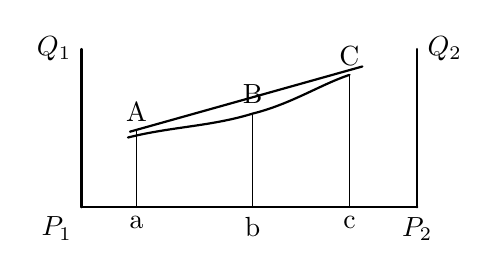
\begin{tikzpicture}[scale=.82, line cap=round,line join=round]
\draw[thick] (0,0) -- (5.2,0) node[below] {$P_2$};
\draw[thick] (0,0) -- (0,2.45) node[left] {$Q_1$};
\draw[thick] (5.2,0) -- (5.2,2.45) node[right] {$Q_2$};
\node[below left] at (0,0) {$P_1$};
\draw (0.85,0) -- (0.85,1.18);
\draw (2.65,0) -- (2.65,1.45);
\draw (4.15,0) -- (4.15,2.05);
\draw[thick] (0.72,1.08) .. controls (1.4,1.25) and (2.0,1.25) .. (2.65,1.45)
             .. controls (3.25,1.6) and (3.7,1.9) .. (4.15,2.05);
\draw[thick] (0.75,1.17) -- (4.35,2.18);
\node[above] at (0.85,1.18) {A};
\node[above] at (2.65,1.45) {B};
\node[above] at (4.15,2.05) {C};
\node[below] at (0.85,0) {a};
\node[below] at (2.65,0) {b};
\node[below] at (4.15,0) {c};
\end{tikzpicture}\\[-0.2em]
{\small Fig. 1.}
\end{center}

Now if we denote by $\eta'$ the entropy of the phase represented by the point B considered as belonging to the curve (B), and by $\eta''$ the entropy of the composite state of the same matter represented by the point B considered as belonging to the tangent to the curves (A) and (C), $t(\eta'-\eta'')$ will denote the heat yielded by a unit of matter in passing from the first to the second of these states. If this quantity is positive, an elevation of temperature will evidently cause a part of the curve (B) to protrude below the tangent to (A) and (C), which will no longer form a part of the line of dissipated energy. This line will then include portions of the three curves (A), (B), and (C), and of the tangents to (A) and (B) and to (B) and (C). On the other hand, a lowering of the temperature will cause the curve (B) to lie entirely above the tangent to (A) and (C), so that all the phases of the sort represented by (B) will be unstable. If $t(\eta'-\eta'')$ is negative, these effects will be produced by the opposite changes of temperature.

The effect of a change of pressure while the temperature remains constant may be found in a manner entirely analogous. The variation of any ordinate will be
\[
\left(\frac{\dd\zeta}{\dd p}\right)_{t,m}\dd p,
\quad\text{or}\quad v\,\dd p.
\]
Therefore, if the volume of the homogeneous phase represented by the point B is greater than the volume of the same matter divided between the phases represented by A and C, an increase of pressure will give a diagram indicating that all phases of the sort represented by curve (B) are unstable, and a decrease of pressure will give a diagram indicating two stable pairs of coexistent phases, in each of which one of the phases is of the sort represented by the curve (B). When the relation of the volumes is the reverse of that supposed, these results will be produced by the opposite changes of pressure.

When we have four coexistent phases of three component substances, there are two cases which must be distinguished. In the first, one of the points of contact of the primitive surface with the quadruple tangent plane lies within the triangle formed by joining the other three; in the second, the four points may be joined so as to form a quadrilateral without re-entrant angles. Figure 2 represents the projection upon the $X$-$Y$ plane (in which $m_1,m_2,m_3$ are measured) of a part of the surface of dissipated energy, when one of the points of contact D falls within the triangle formed by the other three A, B, C. This surface includes the triangle ABC in the quadruple tangent plane, portions of the three sheets of the primitive surface which touch the triangle at its vertices, EAF, GBH, ICK, and portions of the three developable surfaces formed by a tangent plane rolling upon each pair of these sheets. These developable surfaces are represented in the figure by ruled surfaces, the lines indicating the direction of their rectilinear elements. A point within the triangle ABC represents a mass of which the matter is divided, in general, between three or four different phases, in a manner not entirely determined by the position of a point. (The quantities of matter in these phases are such that if placed at the corresponding points, A, B, C, D, their center of gravity would be at the point representing the total mass.) Such a mass, if exposed to constant temperature and pressure, would be in neutral equilibrium. A point in the developable surfaces represents a mass of which the matter is divided between two coexisting phases, which are represented by the extremities of the line in the figure passing through that point. A point in the primitive surface represents of course a homogeneous mass.

To determine the effect of a change of temperature without change of pressure upon the general features of the surface of dissipated energy, we must know whether heat is absorbed or yielded by a mass in passing from the phase represented by the point D in the primitive surface to the composite state consisting of the phases A, B, and C which is represented by the same point. If the first is the case, an increase of temperature will cause the sheet (D) (i.e., the sheet of the primitive surface to which the point D belongs) to separate from the plane tangent to the three other sheets, so as to be situated entirely above it, and a decrease of temperature will cause a part of the sheet (D) to protrude through the plane tangent to the other sheets. These effects will be produced by the opposite changes of temperature, when heat is yielded by a mass passing from the homogeneous to the composite state above mentioned.

In like manner, to determine the effect of a variation of pressure without change of temperature, we must know whether the volume for the homogeneous phase represented by D is greater or less than the volume of the same matter divided between the phases A, B, and C. If the homogeneous phase has the greater volume, an increase of pressure will cause the sheet (D) to separate from the plane tangent to the other sheets, and a diminution of pressure will cause a part of the sheet (D) to protrude below that tangent plane. And these effects will be produced by the opposite changes of pressure, if the homogeneous phase has the less volume. All this appears from precisely the same considerations which were used in the analogous case for two component substances.

\begin{center}
\begin{minipage}{0.46\linewidth}\centering
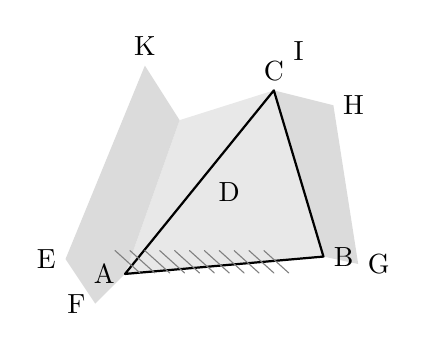
\begin{tikzpicture}[scale=.63,line join=round,line cap=round]
\fill[gray!18] (0,0) -- (4.0,.35) -- (3.0,3.7) -- (1.1,3.1) -- cycle;
\fill[gray!28] (-.6,-.6) -- (0,0) -- (1.1,3.1) -- (.4,4.2) -- (-1.2,.3) -- cycle;
\fill[gray!28] (4.0,.35) -- (4.7,.2) -- (4.2,3.4) -- (3.0,3.7) -- cycle;
\draw[thick] (0,0) node[left]{A} -- (4.0,.35) node[right]{B} -- (3.0,3.7) node[above]{C} -- cycle;
\node at (2.1,1.65) {D};
\node[left] at (-.6,-.6){F}; \node[left] at (-1.2,.3){E}; \node[above] at (.4,4.2){K};
\node[right] at (4.7,.2){G}; \node[right] at (4.2,3.4){H}; \node[above] at (3.5,4.1){I};
\foreach \x in {0.3,0.6,...,3.6} {\draw[gray] (\x,0.02) -- ++(-.5,.45);} 
\end{tikzpicture}\\[-0.2em]{\small Fig. 2.}
\end{minipage}\hfill
\begin{minipage}{0.46\linewidth}\centering
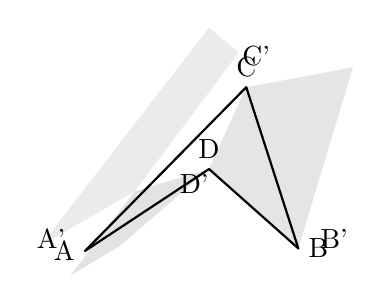
\begin{tikzpicture}[scale=.63,line join=round,line cap=round]
\fill[gray!22] (-.3,-.5) -- (1.0,1.2) -- (2.5,1.65) -- (.7,.1) -- cycle;
\fill[gray!20] (2.5,1.65) -- (4.3,.05) -- (5.4,3.7) -- (3.25,3.3) -- cycle;
\fill[gray!16] (-.9,.1) -- (1.0,1.2) -- (3.1,4.0) -- (2.5,4.5) -- cycle;
\draw[thick] (0,0) node[left]{A} -- (2.5,1.65) node[above]{D} -- (4.3,.05) node[right]{B};
\draw[thick] (0,0) -- (3.25,3.3) node[above]{C} -- (4.3,.05);
\node at (2.2,1.35) {D'}; \node[above] at (3.45,3.55){C'}; \node[right] at (4.55,.25){B'}; \node[left] at (-.2,.25){A'};
\end{tikzpicture}\\[-0.2em]{\small Fig. 3.}
\end{minipage}
\end{center}

Now when the sheet (D) rises above the plane tangent to the other sheets, the general features of the surface of dissipated energy are not altered, except by the disappearance of the point D. But when the sheet (D) protrudes below the plane tangent to the other sheets, the surface of dissipated energy will take the form indicated in figure 3. It will include portions of the four sheets of the primitive surface, portions of the six developable surfaces formed by a double tangent plane rolling upon these sheets taken two by two, and portions of three triple tangent planes for these sheets taken by threes, the sheet (D) being always one of the three.

But when the points of contact with the quadruple tangent plane which represent the four coexistent phases can be joined so as to form a quadrilateral ABCD (fig. 4) without re-entrant angles, the surface of dissipated energy will include this plane quadrilateral, portions of the four sheets of the primitive surface which are tangent to it, and portions of the four developable surfaces formed by double tangent planes rolling upon the four pairs of these sheets which correspond to the four sides of the quadrilateral. To determine the general effect of a variation of temperature upon the surface of dissipated energy, let us consider the composite states represented by the point I at the intersection of the diagonals of the quadrilateral. Among these states (which all relate to the same kind and quantity of matter) there is one which is composed of the phases A and C, and another which is composed of the phases B and D. Now if the entropy of the first of these states is greater than that of the second (i.e., if heat is given out by a body in passing from the first to the second state at constant temperature and pressure), which we may suppose without loss of generality, an elevation of temperature while the pressure remains constant will cause the triple tangent planes to (B), (D), and (A), and to (B), (D), and (C), to rise above the triple tangent planes to (A), (C), and (B), and to (A), (C), and (D), in the vicinity of the point I. The surface of dissipated energy will therefore take the form indicated in figure 5, in which there are two plane triangles and five developable surfaces besides portions of the four primitive sheets. A diminution of temperature will give a different but entirely analogous form to the surface of dissipated energy. The quadrilateral ABCD will in this case break into two triangles along the diameter BD. The effects produced by variation of the pressure while the temperature remains constant will of course be similar to those described. By considering the difference of volume instead of the difference of entropy of the two states represented by the point I in the quadruple tangent plane, we may distinguish between the effects of increase and diminution of pressure.

\begin{center}
\begin{minipage}{0.46\linewidth}\centering
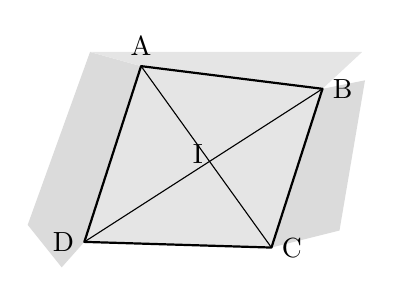
\begin{tikzpicture}[scale=.72,line join=round,line cap=round]
\fill[gray!20] (0,0) -- (1.0,3.1) -- (4.2,2.7) -- (3.3,-.1) -- cycle;
\fill[gray!28] (-.4,-.45) -- (0,0) -- (1.0,3.1) -- (.1,3.35) -- (-1.0,.3) -- cycle;
\fill[gray!28] (4.2,2.7) -- (4.95,2.85) -- (4.5,.2) -- (3.3,-.1) -- cycle;
\fill[gray!20] (.1,3.35) -- (1.0,3.1) -- (4.2,2.7) -- (4.9,3.35) -- cycle;
\draw[thick] (0,0) node[left]{D} -- (1.0,3.1) node[above]{A} -- (4.2,2.7) node[right]{B} -- (3.3,-.1) node[right]{C} -- cycle;
\draw (0,0)--(4.2,2.7); \draw (1.0,3.1)--(3.3,-.1); \node at (2.0,1.55){I};
\end{tikzpicture}\\[-0.2em]{\small Fig. 4.}
\end{minipage}\hfill
\begin{minipage}{0.46\linewidth}\centering
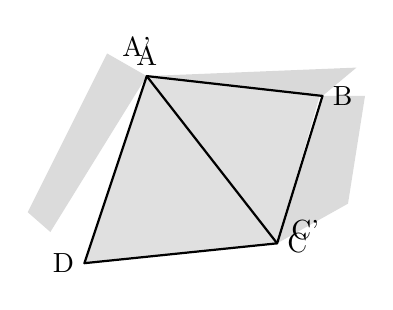
\begin{tikzpicture}[scale=.72,line join=round,line cap=round]
\fill[gray!24] (-.2,-.3) -- (.9,3.0) -- (3.95,2.65) -- (3.2,.05) -- cycle;
\fill[gray!30] (.9,3.0) -- (4.6,3.15) -- (4.0,2.65) -- cycle;
\fill[gray!28] (-.8,.25) -- (.9,3.0) -- (.2,3.4) -- (-1.2,.6) -- cycle;
\fill[gray!28] (4.0,2.65) -- (4.75,2.65) -- (4.45,.75) -- (3.2,.05) -- cycle;
\draw[thick] (-.2,-.3) node[left]{D} -- (.9,3.0) node[above]{A} -- (4.0,2.65) node[right]{B} -- (3.2,.05) node[right]{C} -- cycle;
\draw[thick] (.9,3.0)--(3.2,.05); \node[above] at (.72,3.18){A'}; \node[right] at (3.28,.28){C'};
\end{tikzpicture}\\[-0.2em]{\small Fig. 5.}
\end{minipage}
\end{center}

It should be observed that the points of contact of the quadruple



tangent plane with the primitive surface may be at isolated points or curves belonging to the latter. So also, in the case of two component substances, the points of contact of the triple tangent line may be at isolated points belonging to the primitive curve. Such cases need not be separately treated, as the necessary modifications in the preceding statements, when applied to such cases, are quite evident. And in the remaining discussion of this geometrical method, it will generally be left to the reader to make the necessary limitations or modifications in analogous cases.

The necessary condition in regard to simultaneous variations of temperature and pressure, in order that four coexistent phases of three components, or three coexistent phases of two components, shall remain possible, has already been deduced by purely analytical processes. (See equation (129).)

We will next consider the case of two coexistent phases of identical composition, and first, when the number of components is two. The coexistent phases, if each is variable in composition, will be represented by the point of contact of two curves. One of the curves will in general lie above the other except at the point of contact; therefore, when the temperature and pressure remain constant, one phase cannot be varied in composition without becoming unstable, while the other phase will be stable if the proportion of either component is increased. By varying the temperature or pressure, we may cause the upper curve to protrude below the other, or to rise (relatively) entirely above it. (By comparing the volumes or the entropies of the two coexistent phases, we may easily determine which result would be produced by an increase of temperature or of pressure.) Hence, the temperatures and pressures for which two coexistent phases have the same composition form the limit to the temperatures and pressures for which such coexistent phases are possible. It will be observed that as we pass this limit of temperature and pressure, the pair of coexistent phases does not simply become unstable, like pairs and triads of coexistent phases which we have considered before, but there ceases to be any such pair of coexistent phases. The same result has already been obtained analytically on page 99. But on that side of the limit on which the coexistent phases are possible, there will be two pairs of coexistent phases for the same values of $t$ and $p$, as seen in figure 6.

\begin{center}\label{fig:gibbs-v1-p3-fig6}
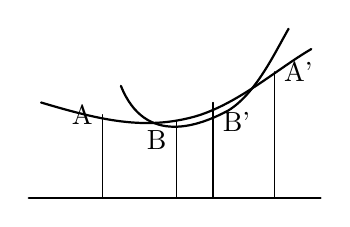
\begin{tikzpicture}[scale=.78,line cap=round,line join=round]
\draw[thick] (-.15,0) -- (4.6,0);
\draw (1.05,0)--(1.05,1.35); \draw (2.25,0)--(2.25,1.25); \draw (2.85,0)--(2.85,1.55); \draw (3.85,0)--(3.85,2.05);
\draw[thick] (.05,1.55) .. controls (1.05,1.25) and (1.75,1.1) .. (2.55,1.32) .. controls (3.25,1.52) and (3.9,2.1) .. (4.45,2.42);
\draw[thick] (1.35,1.82) .. controls (1.75,.82) and (2.65,1.18) .. (3.1,1.42) .. controls (3.55,1.7) and (3.85,2.35) .. (4.08,2.75);
\node[left] at (1.05,1.35) {A};
\node[below left] at (2.25,1.25) {B};
\node[below right] at (2.85,1.55) {B'};
\node[right] at (3.85,2.05) {A'};
\end{tikzpicture}\\[-0.15em]
{\small Fig. 6.}
\end{center}

If the curve AA' represents vapor, and the curve BB' liquid, a liquid (represented by) B may exist in contact with a vapor A, and (at the same temperature and pressure) a liquid B' in contact with a vapor A'. If we compare these phases in respect to their composition, we see that in one case the vapor is richer than the liquid in a certain component, and in the other case poorer. Therefore, if these liquids are made to boil, the effect on their composition will be opposite. If the boiling is continued under constant pressure, the temperature will rise as the liquids approach each other in composition, and the curve BB' will rise relatively to the curve AA', until the curves are tangent to each other, when the two liquids become identical in nature, as also the vapors which they yield. In composition, and in the value of $\zeta$ per unit of mass, the vapor will then agree with the liquid. But if the curve BB' (which has the greater curvature) represents vapor, and AA' represents liquid, the effect of boiling will make the liquids A and A' differ more in composition. In this case, the relations indicated in the figure will hold for a temperature higher than that for which (with the same pressure) the curves are tangent to one another.

When two coexistent phases of three component substances have the same composition, they are represented by the point of contact of two sheets of the primitive surface. If these sheets do not intersect at the point of contact, the case is very similar to that which we have just considered. The upper sheet except at the point of contact represents unstable phases. If the temperature or pressure are so varied that a part of the upper sheet protrudes through the lower, the points of contact of a double tangent plane rolling upon the two sheets will describe a closed curve on each, and the surface of dissipated energy will include a portion of each sheet of the primitive surface united by a ring-shaped developable surface.

If the sheet having the greater curvatures represents liquid, and the other sheet vapor, the boiling temperature for any given pressure will be a maximum, and the pressure of saturated vapor for any given temperature will be a minimum, when the coexistent liquid and vapor have the same composition.

But if the two sheets, constructed for the temperature and pressure of the coexistent phases which have the same composition, intersect at the point of contact, the whole primitive surface as seen from below will in general present four re-entrant furrows, radiating from the point of contact, for each of which a developable surface may be formed by a rolling double tangent plane. The different parts of the surface of dissipated energy in the vicinity of the point of contact are represented in figure 7. ATB, ETF are parts of one sheet of the primitive surface, and CTD, GTH are parts of the other. These are united by the developable surfaces BTC,

\begin{center}\label{fig:gibbs-v1-p3-fig7}
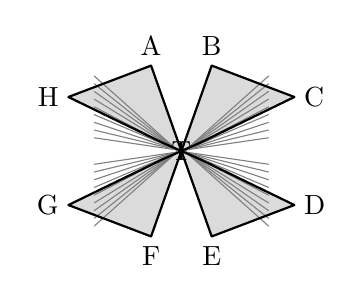
\begin{tikzpicture}[scale=.70,line cap=round,line join=round]
\fill[gray!28] (0,0)--(-.55,1.55)--(-2.05,.98)--(-.34,.15)--cycle;
\fill[gray!28] (0,0)--(.55,1.55)--(2.05,.98)--(.34,.15)--cycle;
\fill[gray!28] (0,0)--(.55,-1.55)--(2.05,-.98)--(.34,-.15)--cycle;
\fill[gray!28] (0,0)--(-.55,-1.55)--(-2.05,-.98)--(-.34,-.15)--cycle;
\foreach \y in {.24,.38,.52,.66,.80,.94,1.08,1.22,1.36} {\draw[gray] (-.08,.02)--(-1.58,\y);}
\foreach \y in {.24,.38,.52,.66,.80,.94,1.08,1.22,1.36} {\draw[gray] (.08,.02)--(1.58,\y);}
\foreach \y in {-.24,-.38,-.52,-.66,-.80,-.94,-1.08,-1.22,-1.36} {\draw[gray] (.08,-.02)--(1.58,\y);}
\foreach \y in {-.24,-.38,-.52,-.66,-.80,-.94,-1.08,-1.22,-1.36} {\draw[gray] (-.08,-.02)--(-1.58,\y);}
\draw[thick] (0,0)--(-.55,1.55)--(-2.05,.98)--(-.34,.15)--cycle;
\draw[thick] (0,0)--(.55,1.55)--(2.05,.98)--(.34,.15)--cycle;
\draw[thick] (0,0)--(.55,-1.55)--(2.05,-.98)--(.34,-.15)--cycle;
\draw[thick] (0,0)--(-.55,-1.55)--(-2.05,-.98)--(-.34,-.15)--cycle;
\node at (0,0) {T};
\node[above] at (-.55,1.55) {A}; \node[left] at (-2.05,.98) {H};
\node[above] at (.55,1.55) {B}; \node[right] at (2.05,.98) {C};
\node[right] at (2.05,-.98) {D}; \node[below] at (.55,-1.55) {E};
\node[left] at (-2.05,-.98) {G}; \node[below] at (-.55,-1.55) {F};
\end{tikzpicture}\\[-0.15em]
{\small Fig. 7.}
\end{center}

DTE, FTG, HTA. Now we may make either sheet of the primitive surface sink relatively to the other by the proper variation of temperature or pressure. If the sheet to which ATB, ETF belong is that which sinks relatively, these parts of the surface of dissipated energy will be merged in one, as well as the developable surfaces BTC, DTE, and also FTG, HTA. (The lines CTD, BTE, ATF, HTG will separate from one another at T, each forming a continuous curve.) But if the sheet of the primitive surface which sinks relatively is that to which CTD and GTH belong, then these parts will be merged in one in the surface of dissipated energy, as will be the developable surfaces BTC, ATH, and also DTE, FTG.

It is evident that this is not a case of maximum or minimum temperature for coexistent phases under constant pressure, or of maximum or minimum pressure for coexistent phases at constant temperature.

Another case of interest is when the composition of one of three coexistent phases is such as can be produced by combining the other two. In this case, the primitive surface must touch the same plane in three points in the same straight line. Let us distinguish the parts of the primitive surface to which these points belong as the sheets (A), (B), and (C), (C) denoting that which is intermediate in position. The sheet (C) is evidently tangent to the developable surface formed upon (A) and (B). It may or it may not intersect it at the point of contact. If it does not, it must lie above the developable surface (unless it represents states which are unstable in regard to continuous changes), and the surface of dissipated energy will include parts of the primitive sheets (A) and (B), the developable surface joining them, and the single point of the sheet (C) in which it meets this developable surface. Now, if the temperature or pressure is varied so as to make the sheet (C) rise above the developable surface formed on the sheets (A) and (B), the surface of dissipated energy will be altered in its general features only by the removal of the single point of the sheet (C). But if the temperature or pressure is altered so as to make a part of the sheet (C) protrude through the developable surface formed on (A) and (B), the surface of dissipated energy will have the form indicated in figure 8.

\begin{center}\label{fig:gibbs-v1-p3-fig8}
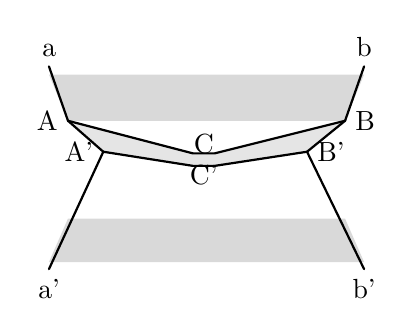
\begin{tikzpicture}[scale=.69,line cap=round,line join=round]
\fill[gray!30] (0,2.2) -- (5.8,2.2) -- (5.45,1.35) -- (.35,1.35) -- cycle;
\fill[gray!20] (.35,1.35) -- (2.65,.75) -- (3.05,.75) -- (5.45,1.35) -- (4.75,.78) -- (3.05,.52) -- (2.65,.52) -- (1.0,.78) -- cycle;
\fill[gray!30] (.35,-.45) -- (5.45,-.45) -- (5.8,-1.25) -- (0,-1.25) -- cycle;
\draw[thick] (0,2.35) node[above]{a} -- (.35,1.35) node[left]{A} -- (1.0,.78) node[left]{A'} -- (0,-1.38) node[below]{a'};
\draw[thick] (5.8,2.35) node[above]{b} -- (5.45,1.35) node[right]{B} -- (4.75,.78) node[right]{B'} -- (5.8,-1.38) node[below]{b'};
\draw[thick] (.35,1.35)--(2.65,.75)--(3.05,.75)--(5.45,1.35);
\draw[thick] (1.0,.78)--(2.65,.52)--(3.05,.52)--(4.75,.78);
\node at (2.85,.92) {C}; \node at (2.85,.35) {C'};
\end{tikzpicture}\\[-0.15em]
{\small Fig. 8.}
\end{center}

It will include two plane triangles ABC and A'B'C', a part of each of the sheets (A) and (B), represented in the figure by the spaces on the left of the line aAA'a' and on the right of the line bBB'b', a small part CC' of the sheet (C), and developable surfaces formed upon these sheets taken by pairs ACC'A', BCC'B', aABb, a'A'B'b', the last two being different portions of the same developable surface.

But if, when the primitive surface is constructed for such a temperature and pressure that it has three points of contact with the same plane in the same straight line, the sheet (C) (which has the middle position) at its point of contact with the triple tangent plane intersects the developable surface formed upon the other sheets (A) and (B), the surface of dissipated energy will not include this developable surface, but will consist of portions of the three primitive sheets with two developable surfaces formed on (A) and (C) and on (B) and (C). These developable surfaces meet one another at the point of contact of (C) with the triple tangent plane, dividing the portion of this sheet which belongs to the surface of dissipated energy into two parts. If now the temperature or pressure are varied so as to make the sheet (C) sink relatively to the developable surface formed on (A) and (B), the only alteration in the general features of the surface of dissipated energy will be that the developable surfaces formed on (A) and (C) and on (B) and (C) will separate from one another, and the two parts of the sheet (C) will be merged in one. But a contrary variation of temperature or pressure will give a surface of dissipated energy such as is represented in figure (9), containing two plane triangles ABC, A'B'C' belonging to triple tangent planes,

\begin{center}\label{fig:gibbs-v1-p3-fig9}
\begin{minipage}{0.50\linewidth}\centering
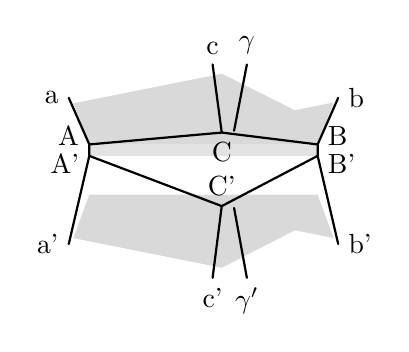
\begin{tikzpicture}[scale=.58,line cap=round,line join=round]
\fill[gray!30] (.1,1.6)--(3.35,2.25)--(4.95,1.45)--(5.8,1.62)--(5.45,.7)--(.45,.7)--cycle;
\fill[gray!22] (.45,.7)--(5.45,.7)--(5.45,.45)--(.45,.45)--cycle;
\fill[gray!30] (.45,-.4)--(5.45,-.4)--(5.8,-1.35)--(4.95,-1.18)--(3.35,-2.0)--(.1,-1.35)--cycle;
\draw[thick] (0,1.72) node[left]{a} -- (.45,.7) node[left,yshift=3pt]{A} -- (.45,.45) node[left,yshift=-3pt]{A'} -- (0,-1.48) node[left]{a'};
\draw[thick] (5.9,1.72) node[right]{b} -- (5.45,.7) node[right,yshift=3pt]{B} -- (5.45,.45) node[right,yshift=-3pt]{B'} -- (5.9,-1.48) node[right]{b'};
\draw[thick] (3.15,2.45) node[above]{c} -- (3.35,.96) node[below]{C};
\draw[thick] (3.9,2.45) node[above]{$\gamma$} -- (3.62,1.0);
\draw[thick] (3.35,-.65) node[above]{C'} -- (3.15,-2.22) node[below]{c'};
\draw[thick] (3.62,-.69) -- (3.9,-2.22) node[below]{$\gamma'$};
\draw[thick] (.45,.7)--(3.35,.96)--(5.45,.7);
\draw[thick] (.45,.45)--(3.35,-.65)--(5.45,.45);
\end{tikzpicture}\\[-0.15em]
{\small Fig. 9.}
\end{minipage}
\end{center}

a portion of the sheet (A) on the left of the line aAA'a', a portion of the sheet (B) on the right of the line bBB'b', two separate portions cC$\gamma$ and c'C'$\gamma'$ of the sheet (C), two separate portions aACc and a'A'C'c' of the developable surface formed on (A) and (C), two separate portions bBC$\gamma$ and b'B'C'$\gamma'$ of the developable surface formed on (B) and (C), and the portion A'ABB' of the developable surface formed on (A) and (B).

From these geometrical relations it appears that (in general) the temperature of three coexistent phases is a maximum or minimum for constant pressure, and the pressure of three coexistent phases a maximum or minimum for constant temperature, when the composition of the three coexistent phases is such that one can be formed by combining the other two. This result has been obtained analytically on page 99.

The preceding examples are amply sufficient to illustrate the use of the $m$-$\zeta$ surfaces and curves. The physical properties indicated by the nature of the surface of dissipated energy have been only occasionally mentioned, as they are often far more distinctly indicated by the diagrams than they could be in words. It will be observed that a knowledge of the lines which divide the various different portions of the surface of dissipated energy and of the direction of the rectilinear elements of the developable surfaces, \emph{as projected upon the $X$-$Y$ plane}, without a knowledge of the form of the $m$-$\zeta$ surface in space, is sufficient for the determination (in respect to the quantity and composition of the resulting masses) of the combinations and separations of the substances, and of the changes in their states of aggregation, which take place when the substances are exposed to the temperature and pressure to which the projected lines relate, except so far as such transformations are prevented by passive resistances to change.

\section*{Critical Phases}

It has been ascertained by experiment that the variations of two coexistent states of the same substance are in some cases limited in one direction by a terminal state at which the distinction of the coexistent states vanishes.\symfootnote{*}{See Dr. Andrews ``On the continuity of the gaseous and liquid states of matter.'' \textit{Phil. Trans.}, vol. 159, p. 575.} This state has been called the \textit{critical state}. Analogous properties may doubtless be exhibited by compounds of variable composition without change of temperature or pressure. For if, at any given temperature and pressure, two liquids are capable of forming a stable mixture in any ratio $m_1:m_2$ less than $a$, and in any greater than $b$, $a$ and $b$ being the values of that ratio for two coexistent phases, while either can form a stable mixture with a third liquid in all proportions, and any small quantities of the first and second can unite at once with a great quantity of the third to form a stable mixture, it may easily be seen that two coexistent mixtures of the three liquids may be varied in composition, the temperature and pressure remaining the same, from initial phases in each of which the quantity of the third liquid is nothing, to a terminal phase in which the distinction of the two phases vanishes.

In general, we may define a \textit{critical phase} as one at which the distinction between coexistent phases vanishes. We may suppose the coexistent phases to be stable in respect to continuous changes, for although relations in some respects analogous might be imagined to hold true in regard to phases which are unstable in respect to continuous changes, the discussion of such cases would be devoid of interest. But if the coexistent phases and the critical phase are unstable only in respect to the possible formation of phases entirely different from the critical and adjacent phases, the liability to such changes will in no respect affect the relations between the critical and adjacent phases, and need not be considered in a theoretical discussion of these relations, although it may prevent an experimental realization of the phases considered. For the sake of brevity, in the following discussion, phases in the vicinity of the critical phase will generally be called stable, if they are unstable only in respect to the formation of phases entirely different from any in the vicinity of the critical phase.

Let us first consider the number of independent variations of which a critical phase (while remaining such) is capable. If we denote by $n$ the number of independently variable components, a pair of coexistent phases will be capable of $n$ independent variations, which may be expressed by the variations of $n$ of the quantities $t,p,\mu_1,\mu_2,\ldots,\mu_n$. If we limit these variations by giving to $n-1$ of the quantities the constant values which they have for a certain critical phase, we obtain a linear\symfootnote{*}{This term is used to characterize a series having a single degree of extension.} series of pairs of coexistent phases terminated by the critical phase. If we now vary infinitesimally the values of these $n-1$ quantities, we shall have for the new set of values considered constant a new linear series of pairs of coexistent phases. Now for every pair of phases in the first series, there must be pairs of phases in the second series differing infinitely little from the pair in the first, and vice versa, therefore the second series of coexistent phases must be terminated by a critical phase which differs, but differs infinitely little, from the first. We see, therefore, that if we vary arbitrarily the values of any $n-1$ of the quantities, $t,p,\mu_1,\mu_2,\ldots,\mu_n$, as determined by a critical phase, we obtain one and only one critical phase for each set of varied values; i.e., a critical phase is capable of $n-1$ independent variations.

The quantities $t,p,\mu_1,\mu_2,\ldots,\mu_n$ have the same values in two coexistent phases, but the ratios of the quantities $\eta,v,m_1,m_2,\ldots,m_n$ are in general different in the two phases. Or, if for convenience we compare equal volumes of the two phases (which involves no loss of generality), the quantities $\eta,m_1,m_2,\ldots,m_n$ will in general have different values in two coexistent phases. Applying this to coexistent phases indefinitely near to a critical phase, we see that in the immediate vicinity of a critical phase, if the values of $n$ of the quantities $t,p,\mu_1,\mu_2,\ldots,\mu_n$ are regarded as constant (as well as $v$), the variations of either of the others will be infinitely small compared with the variations of the quantities $\eta,m_1,m_2,\ldots,m_n$. This condition, which we may write in the form
\begin{equation}\label{eq:gibbs-v1-p3-200}
\left(\frac{\dd\mu_n}{\dd m_n}\right)_{t,v,\mu_1,\ldots,\mu_{n-1}}=0,
\tag{200}
\end{equation}
characterizes, as we have seen on page 114, the limits which divide stable from unstable phases in respect to continuous changes.

In fact, if we give to the quantities $t,\mu_1,\mu_2,\ldots,\mu_{n-1}$ constant values determined by a pair of coexistent phases, and to $m_n/v$ a series of values increasing from the less to the greater of the values which it has in these coexistent phases, we determine a linear series of phases connecting the coexistent phases, in some part of which $\mu_n$---since it has the same value in the two coexistent phases, but not a uniform value throughout the series (for if it had, which is theoretically improbable, all these phases would be coexistent)---must be a decreasing function of $m_n/v$, or of $m_n$, if $v$ also is supposed constant. Therefore, the series must contain phases which are unstable in respect to continuous changes. (See page 111.) And as such a pair of coexistent phases may be taken indefinitely near to any critical phase, the unstable phases (with respect to continuous changes) must approach indefinitely near to this phase.

Critical phases have similar properties with reference to stability as determined with regard to discontinuous changes. For as every stable phase which has a coexistent phase lies upon the limit which separates stable from unstable phases, the same must be true of any stable critical phase. (The same may be said of critical phases which are unstable in regard to discontinuous changes, if we leave out of account the liability to the particular kind of discontinuous change in respect to which the critical phase is unstable.)

The linear series of phases determined by giving to $n$ of the quantities $t,p,\mu_1,\mu_2,\ldots,\mu_n$ the constant values which they have in any pair of coexistent phases consists of unstable phases in the part between the coexistent phases, but in the part beyond these phases in either direction it consists of stable phases. Hence, if a critical phase is varied in such a manner that $n$ of the quantities $t,p,\mu_1,\mu_2,\ldots,\mu_n$ remain constant, it will remain stable in respect both to continuous and to discontinuous changes. Therefore $\mu_n$ is an increasing function of $m_n$ when $t,v,\mu_1,\mu_2,\ldots,\mu_{n-1}$ have constant values determined by any critical phase. But as equation (200) holds true at the critical phase, the following conditions must also hold true at that phase:---
\begin{align}
\left(\frac{\dd^2\mu_n}{\dd m_n^2}\right)_{t,v,\mu_1,
\ldots,\mu_{n-1}}&=0, \tag{201}\label{eq:gibbs-v1-p3-201}\\
\left(\frac{\dd^3\mu_n}{\dd m_n^3}\right)_{t,v,\mu_1,
\ldots,\mu_{n-1}}&\geq 0. \tag{202}\label{eq:gibbs-v1-p3-202}
\end{align}
If the sign of equality holds in the last condition, additional conditions, concerning the differential coefficients of higher orders, must be satisfied.

Equations (200) and (201) may in general be called the equations of critical phases. It is evident that there are only two independent equations of this character, as a critical phase is capable of $n-1$ independent variations.

We are not, however, absolutely certain that equation (200) will always be satisfied by a critical phase. For it is possible that the denominator in the fraction may vanish as well as the numerator for an infinitesimal change of phase in which the quantities indicated are constant. In such a case, we may suppose the subscript $n$ to refer to some different component substance, or use another differential coefficient of the same general form (such as are described on page 114 as characterizing the limits of stability in respect to continuous changes), making the corresponding changes in (201) and (202). We may be certain that some of the formulae thus formed will not fail. But for a perfectly rigorous method there is an advantage in the use of $\eta,v,m_1,m_2,\ldots,m_n$ as independent variables. The condition that the phase may be varied without altering any of the quantities $t,\mu_1,\mu_2,\ldots,\mu_n$ will then be expressed by the equation
\begin{equation}\label{eq:gibbs-v1-p3-203}
R_{n+1}=0,
\tag{203}
\end{equation}
in which $R_{n+1}$ denotes the same determinant as on page 111. To obtain the second equation characteristic of critical phases, we observe that as a phase which is critical cannot become unstable when varied so that $n$ of the quantities $t,p,\mu_1,\mu_2,\ldots,\mu_n$ remain constant, the differential of $R_{n+1}$ for constant volume, viz.,
\begin{equation}\label{eq:gibbs-v1-p3-204}
\frac{\dd R_{n+1}}{\dd\eta}\dd\eta
+\frac{\dd R_{n+1}}{\dd m_1}\dd m_1
+\cdots+
\frac{\dd R_{n+1}}{\dd m_n}\dd m_n,
\tag{204}
\end{equation}
cannot become negative when $n$ of the equations (172) are satisfied. Neither can it have a positive value, for then its value might become negative by a change of sign of $\dd\eta,\dd m_1$, etc. Therefore the expression (204) has the value zero, if $n$ of the equations (172) are satisfied. This may be expressed by an equation
\begin{equation}\label{eq:gibbs-v1-p3-205}
S=0,
\tag{205}
\end{equation}
in which $S$ denotes a determinant in which the constituents are the same as in $R_{n+1}$, except in a single horizontal line, in which the differential coefficients in (204) are to be substituted. In whatever line this substitution is made, the equation (205), as well as (203), will hold true of every critical phase without exception.

If we choose $t,p,m_1,m_2,\ldots,m_n$ as independent variables, and write $U$ for the determinant
\begin{equation}\label{eq:gibbs-v1-p3-206}
\left|
\begin{array}{cccc}
\dfrac{\dd^2\zeta}{\dd m_1^2} &
\dfrac{\dd^2\zeta}{\dd m_2\dd m_1} & \cdots &
\dfrac{\dd^2\zeta}{\dd m_{n-1}\dd m_1}\\[0.9em]
\dfrac{\dd^2\zeta}{\dd m_1\dd m_2} &
\dfrac{\dd^2\zeta}{\dd m_2^2} & \cdots &
\dfrac{\dd^2\zeta}{\dd m_{n-1}\dd m_2}\\
\cdots & \cdots & \cdots & \cdots\\
\dfrac{\dd^2\zeta}{\dd m_1\dd m_{n-1}} &
\dfrac{\dd^2\zeta}{\dd m_2\dd m_{n-1}} & \cdots &
\dfrac{\dd^2\zeta}{\dd m_{n-1}^2}
\end{array}
\right|,
\tag{206}
\end{equation}
and $V$ for the determinant formed from this by substituting for the constituents in any horizontal line the expressions
\begin{equation}\label{eq:gibbs-v1-p3-207}
\frac{\dd U}{\dd m_1},\quad
\frac{\dd U}{\dd m_2},\quad \ldots \quad
\frac{\dd U}{\dd m_{n-1}},
\tag{207}
\end{equation}
the equations of critical phases will be
\begin{equation}\label{eq:gibbs-v1-p3-208}
U=0,\qquad V=0.
\tag{208}
\end{equation}

It results immediately from the definition of a critical phase, that an infinitesimal change in the condition of a mass in such a phase may cause the mass, if it remains in a state of dissipated energy (i.e., in a state in which the dissipation of energy, by internal processes is complete), to cease to be homogeneous. In this respect a critical phase resembles any phase which has a coexistent phase, but differs from such phases in that the two parts into which the mass divides when it ceases to be homogeneous differ infinitely little from each other and from the original phase, and that neither of these parts is in general infinitely small. If we consider a change in the mass to be determined by the values of $\dd\eta,\dd v,\dd m_1,\dd m_2,\ldots,\dd m_n$, it is evident that the change in question will cause the mass to cease to be homogeneous whenever the expression
\begin{equation}\label{eq:gibbs-v1-p3-209}
\frac{\dd R_{n+1}}{\dd\eta}\dd\eta
+\frac{\dd R_{n+1}}{\dd v}\dd v
+\frac{\dd R_{n+1}}{\dd m_1}\dd m_1
+\cdots+
\frac{\dd R_{n+1}}{\dd m_n}\dd m_n
\tag{209}
\end{equation}
has a negative value. For if the mass should remain homogeneous, it would become unstable, as $R_{n+1}$ would become negative. Hence, in general, any change thus determined, or its reverse (determined by giving to $\dd\eta,\dd v,\dd m_1,\dd m_2,\ldots,\dd m_n$ the same values taken negatively), will cause the mass to cease to be homogeneous. The condition which must be satisfied with reference to $\dd\eta,\dd v,\dd m_1,\dd m_2,\ldots,\dd m_n$, in order that neither the change indicated, nor the reverse, shall destroy the homogeneity of the mass, is expressed by equating the above expression to zero.

But if we consider the change in the state of the mass (supposed to remain in a state of dissipated energy) to be determined by arbitrary values of $n+1$ of the differentials $\dd t,\dd p,\dd\mu_1,\dd\mu_2,\ldots,\dd\mu_n$, the case will be entirely different. For, if the mass ceases to be homogeneous, it will consist of two coexistent phases, and as applied to these, only $n$ of the quantities $t,p,\mu_1,\mu_2,\ldots,\mu_n$ will be independent. Therefore, for arbitrary variations of $n+1$ of these quantities, the mass must in general remain homogeneous.

But if, instead of supposing the mass to remain in a state of dissipated energy, we suppose that it remains homogeneous, it may easily be shown that to certain values of $n+1$ of the above differentials there will correspond three different phases, of which one is stable with respect both to continuous and to discontinuous changes, another is stable with respect to the former and unstable with respect to the latter, and the third is unstable with respect to both.

In general, however, if $n$ of the quantities $p,t,\mu_1,\mu_2,\ldots,\mu_n$, or $n$ arbitrary functions of these quantities, have the same constant values as at a critical phase, the linear series of phases thus determined will be stable, in the vicinity of the critical phase. But if less than $n$ of these quantities or functions of the same together with certain of the quantities $\eta,v,m_1,m_2,\ldots,m_n$, or arbitrary functions of the latter quantities, have the same values as at a critical phase, so as to determine a linear series of phases, the differential of $R_{n+1}$ in such a series of phases will not in general vanish at the critical phase, so that in general a part of the series will be unstable.

We may illustrate these relations by considering separately the cases in which $n=1$ and $n=2$. If a mass of invariable composition is in a critical state, we may keep its volume constant, and destroy its homogeneity by changing its entropy (i.e., by adding or subtracting heat---probably the latter), or we may keep its entropy constant and destroy its homogeneity by changing its volume; but if we keep its pressure constant we cannot destroy its homogeneity by any thermal action, nor if we keep its temperature constant can we destroy its homogeneity by any mechanical action.

When a mass having two independently variable components is in a critical phase, and either its volume or its pressure is maintained constant, its homogeneity may be destroyed by a change of entropy or temperature. Or, if either its entropy or its temperature is maintained constant, its homogeneity may be destroyed by a change of volume or pressure. In both these cases it is supposed that the quantities of the components remain unchanged. But if we suppose both the temperature and the pressure to be maintained constant, the mass will remain homogeneous, however the proportion of the components be changed. Or, if a mass consists of two coexistent phases, one of which is a critical phase having two independently variable components, and either the temperature or the pressure of the mass is maintained constant, it will not be possible by mechanical or thermal means, or by changing the quantities of the components, to cause the critical phase to change into a pair of coexistent phases, so as to give three coexistent phases in the whole mass. The statements of this paragraph and of the preceding have reference only to infinitesimal changes.\symfootnote{*}{A brief abstract (which came to the author's notice after the above was in type) of a memoir by M. Duclaux, ``Sur la séparation des liquides mélangés, etc.'' will be found in \textit{Comptes Rendus}, vol. lxxxi. (1875), p. 815.}

\end{document}
